\documentclass[ENG]{TFUOC}%IB: CASTELLÀ, CAT: CATALÀ, ENG: ENGLISH
\usepackage{amsmath}

% Robust line breaks for long URLs/DOIs in references and text
\PassOptionsToPackage{hyphens}{url}
\usepackage{xurl}
\usepackage{microtype}
\usepackage{float}
\usepackage[authoryear,round]{natbib}
\usepackage{pdflscape}

% Prevent right-margin overflow (overfull hboxes) in difficult lines
\emergencystretch=3em

% Espacio vertical entre párrafos
\setlength{\parskip}{0.6em}   % prueba 0.4em–1em
\setlength{\parindent}{0pt}   % opcional: sin sangría de primera línea

%Introduce Work Data
\title{Comparative Evaluation of Satellite Image Segmentation Methods for Coastline Extraction: Spectral Indices vs. Deep Learning.}
\titcrt{} %Short title to appear in header
\author{Albert Gallego Jiménez}
\date{\today}

\nomPDC{Carlos Cabezas Rabadán and Joaquín Torres Sospedra}
\nomPRA{David Masip Rodó}
\titulac{MSc in Data Science}
\area{Area 4: Pattern Recognition and Computer Vision in Applied Sciences - Geographic Information Systems, satellite images and geopositioning}
\idioma{English}
\credits{15}
\parcla{Earth Observation, Satellite imagery, Coastal Remote Sensing, Semantic Segmentation, Spectral Indices, Water Segmentation}

\licenc{ccBy}
%Possible licenses
%ccByNcNd
%ccByNcSa
%ccByNc
%ccByNd
%ccBySa
%ccBy
%GNU
%copyright


%%%%%%%%%%
% Summary in language

\abstractidioma{
Maximum 250 words, for the purpose, context of application, methodology, results and conclusions of the work.
}

% Summary in English.
\abstractenglish{
A maximum of 250 words, detailing the purpose, context of application, methodology, results and conclusions of the work.
}

\begin{document}

\estructura

\tableofcontents

\listoffigures

\listoftables




\chapter{Introduction}

\section{Context and Justification of Work}

Coastal regions are among the most dynamic, densely populated, and socio-economically vital areas on Earth. However, these environments are under constant threat from both natural processes and anthropogenic pressures, exacerbated by climate change. As sea levels rise and extreme weather events become more frequent, coastal erosion has emerged as a critical global challenge. Consequently, accurate and continuous monitoring of shoreline position (the instantaneous interface between land and water) is essential for understanding morphological changes, evaluating erosion trends, and planning effective coastal defense strategies.

Historically, tracking shoreline evolution relied on in-situ topographic surveys or aerial photogrammetry. While highly accurate, these methods are often prohibitively expensive, labor-intensive, and limited in spatial and temporal coverage. In recent decades, the advent of Earth Observation (EO) satellites has revolutionized coastal surveying. Missions such as the European Space Agency's (ESA) Sentinel-2 offer free, high-frequency, and multi-decadal imagery spanning the entire globe \citep{vitousek_future_2023}. This wealth of optical satellite data allows researchers and coastal managers to monitor shoreline dynamics at unprecedented scales and at a fraction of the cost.

To extract the exact position of the waterline from a satellite image, traditional methodologies rely heavily on Spectral Indices. These mathematical formulas exploit the differences in how water and land reflect specific bands of sunlight (such as the near-infrared) to create binary masks separating water from non-water. Frameworks utilizing these principles, such as CoastSat \citep{vos_coastsat_2019}, SHOREX \citep{sanchez-garcia_efficient_2020}, and CASSIE \citep{almeida_coastal_2021}, have become the operational standard for generating automated, large-scale shoreline extraction data worldwide, providing an efficient alternative to manual digitization.


However, this traditional pixel-by-pixel approach faces severe limitations when applied to highly dynamic, macrotidal environments. In high-energy coasts with large tidal ranges (such as the Cantabrian Sea) the presence of extensive wet sand and breaking wave foam creates a persistent ``semantic ambiguity''. The basic spectral premise that water strongly absorbs light while land reflects it frequently breaks down in these transition zones, leading to severe misidentifications of the actual waterline (see Figure~\ref{fig:misidentification_example}). As demonstrated by recent studies (e.g., \citealp{cabezas_site-specific_2026}), traditional tools struggle to navigate these challenging coastal scenes, resulting in significant spatial errors.

\begin{figure}[H]
    \centering
    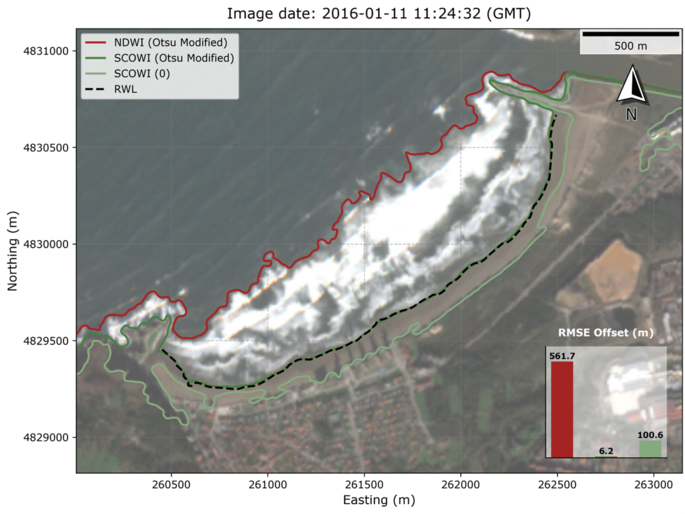
\includegraphics[width=15truecm]{shoreline_misidentification_example.png}
    \caption{Examples of shoreline misidentification in a macrotidal beach (adapted from \citealp{cabezas_site-specific_2026})}
    \label{fig:misidentification_example}
\end{figure}

Consequently, there is a clear and urgent need to move beyond purely spectral formulas and explore methodologies capable of understanding the context of the image. Deep Learning (DL), a subset of Artificial Intelligence (AI), offers a promising solution to bridge this gap. Unlike traditional index thresholds that evaluate the reflectance value of an isolated pixel, advanced DL semantic segmentation architectures can learn complex spatial patterns, textures, and contextual hierarchies. By emulating how the human eye interprets a satellite image (recognizing the texture of a wave or the gradient of wet sand) DL models hold the potential to overcome the spectral confusion inherent in macrotidal environments.

\section{Work Objectives}

Given the challenges posed by macrotidal coasts and the limitations of traditional spectral methods, the overarching goal of this Master's Thesis is to evaluate the operational viability of Deep Learning solutions for shoreline mapping. To ensure a robust assessment, the study will focus on three highly dynamic beaches located along the northern Spanish coast: Salinas (Asturias) and El Puntal (Cantabria). 

\vspace{0.3cm}
\noindent\textbf{Primary Objective:}
\begin{itemize}
    \item To perform a comprehensive benchmarking analysis between traditional spectral-based thresholding (e.g., NDWI, MNDWI) and modern Deep Learning-based semantic segmentation for automated coastline extraction in complex coastal environments.
\end{itemize}

\noindent\textbf{Secondary Objectives:}
\begin{itemize}
    \item To generate a high-quality ``Ground Truth'' dataset of coastal masks (classifying pixels into \textit{water}, \textit{white-water}, \textit{wet sand}, and \textit{sand}). This dataset will be used exclusively to train and validate the Deep Learning segmentation models, and will be rigidly constructed through manual photo-interpretation, utilizing AI-assisted annotation tools (such as the Segment Anything Model, SAM \citep{kirillov_segment_2023}) solely to refine and accelerate the process.
    \item To generate a high-quality ``Ground Truth'' dataset of photo-interpreted waterlines directly derived from the Sentinel-2 imagery. This dataset will serve primarily to benchmark the accuracy of the extracted waterlines (testing both traditional spectral indices-based models and Deep Learning segmentation models).
    \item To systematically evaluate and compare the performance degradation of both classical indices and Neural Networks under specifically adverse oceanographic and atmospheric conditions (e.g., the presence of extensive white foam, variations in intertidal sand moisture, and partial cloud cover).
\end{itemize}

\section{Impact on Sustainability, Ethics-Social and Diversity}
\label{s:etic}

In compliance with the UOC's cross-disciplinary competence ``Ethical and global commitment'', this section identifies the positive and/or negative impacts of the Master's Thesis on the three dimensions: Sustainability, Ethical Behavior and Social Responsibility, and Diversity and Human Rights.

\textbf{1. Sustainability} \\
The project uses freely available Sentinel-2 Level-2A imagery from the Copernicus program and performs all processing either locally or on an institutional computing cluster. Traditional field-based coastal monitoring requires repeated physical surveys with vehicles, boats or aircraft, generating higher operational GHG emissions. The Deep Learning training phase incurs moderate energy consumption inherent to GPU usage; however, this is limited in scope and offset by the elimination of on-site campaigns. No other significant negative environmental impacts (resource depletion, waste generation or large-scale land use) are identified.

Overall impact: neutral to slightly positive.

\textbf{2. Ethical Behavior and Social Responsibility (RS)} \\
All data used are open-access satellite products with no personal, sensitive or identifiable information. Ground-truth masks were generated through manual photo-interpretation assisted only by the Segment Anything Model for refinement. Model performance is evaluated with transparent metrics (IoU, Dice, geometric error) and limitations under adverse conditions (foam, wet sand, clouds) are explicitly quantified and reported. The project does not produce automated decisions affecting individuals or communities. Potential risk of misinterpretation of shoreline outputs by end-users is mitigated by providing full error analysis.

Overall impact: neutral.

\textbf{3. Diversity and Human Rights} \\
The thesis is strictly technical and involves no human subjects, personal data, biometric information or gender-related variables. Development was carried out individually with no team composition. The resulting code, models and documentation use objective technical language and do not contain implicit biases. No positive or negative impacts on human rights, gender diversity or vulnerable groups are identified.

Overall impact: neutral.

\section{Focus and Method Followed}

To address the goal of automating and improving shoreline extraction from Sentinel-2 satellite imagery, several strategies were initially considered. One theoretical approach could involve developing a completely novel Deep Learning architecture from scratch, comprehensively designed for water-sand segmentation. Conversely, an entirely applied approach could rely on utilizing existing proprietary software or closed-source commercial solutions.

However, the chosen strategy for this thesis is an applied comparative benchmarking approach. Rather than inventing a new architecture, this work focuses on adapting and fine-tuning existing, state-of-the-art open-source Deep Learning architectures (such as the U-Net with varying feature-extraction encoders) and rigorously evaluating them against widely adopted traditional baselines (e.g., spectral indices combined with Marching Squares sub-pixel contouring). 

This comparative framework was selected to maximize both practical impact and scientific rigor. At present, the primary challenge in automated shoreline monitoring lies not in developing novel algorithms, but in validating existing state-of-the-art models through standardized coastal metrics. By embedding established semantic segmentation networks into a highly specialized evaluation pipeline, this work shifts the focus from model creation to operational viability and sub-pixel accuracy. Consequently, this ensures a transparent methodology capable of answering the fundamental research question (the operational superiority of Deep Learning over traditional spectral methods) without redundant efforts in foundational architectural design.

\section{Work Schedule}

The project is planned to be developed over a 5-month period (including the thesis defence), structured into the following tasks as shown in the Gantt chart (Figure~\ref{fig:gantt}). Additionally, project management software such as Trello or MS Planner will be used to track and control the tasks at a more specific level:
\begin{itemize}
    \item \textbf{Task 1:} Literature review, selection of study sites (beaches), and satellite images download.
    \begin{itemize}
        \item Literature review on traditional methods for satellite-derived coastline extraction.
        \item Literature review on Deep Learning models applied to coastal monitoring.
        \item Satellite images download for northern Spanish coast beaches: Salinas (Asturias) and El Puntal (Cantabria).
    \end{itemize}
    \item \textbf{Task 2:} Calculation of spectral indices and generation of Ground Truth datasets.
    \begin{itemize}
        \item Preparation of the GitHub repository structure for the project's codebase.
        \item Calculation of spectral indices (e.g., NDWI, MNDWI).
        \item Create RGB composites to assist in the annotation process.
        \item Ground Truth generation through manually photo-interpretation of the RGB composites.
        \item Generation of Ground Truth coastline vectors directly from the Sentinel-2 images, to be used for benchmarking.
    \end{itemize}
    \item \textbf{Task 3:} Model implementation: Development of baseline and Deep Learning architectures.
    \begin{itemize}
        \item Application of automatic thresholding to spectral indices to set baseline models.
        \item Selection, development, and training of Deep Learning architectures.
        \item Application of contouring algorithms to extract shorelines at sub-pixel precision.
    \end{itemize}
    \item \textbf{Task 4:} Statistical analysis of results, benchmarking across different algorithms, and final evaluation.
    \begin{itemize}
        \item Pixel-based metrics evaluation (e.g., IoU, Dice Coefficient).
        \item Geometric validation by calculating the mean Euclidean distance between predicted and real shorelines.
        \item Comparison of performance under adverse conditions (foam, wet sand) and transferability assessment.
    \end{itemize}
    \item \textbf{Task 5:} Drafting report and interim deliveries.
    \item \textbf{Task 6:} Progress meetings with directors.
\end{itemize}

\begin{figure}[H]
    \centering
    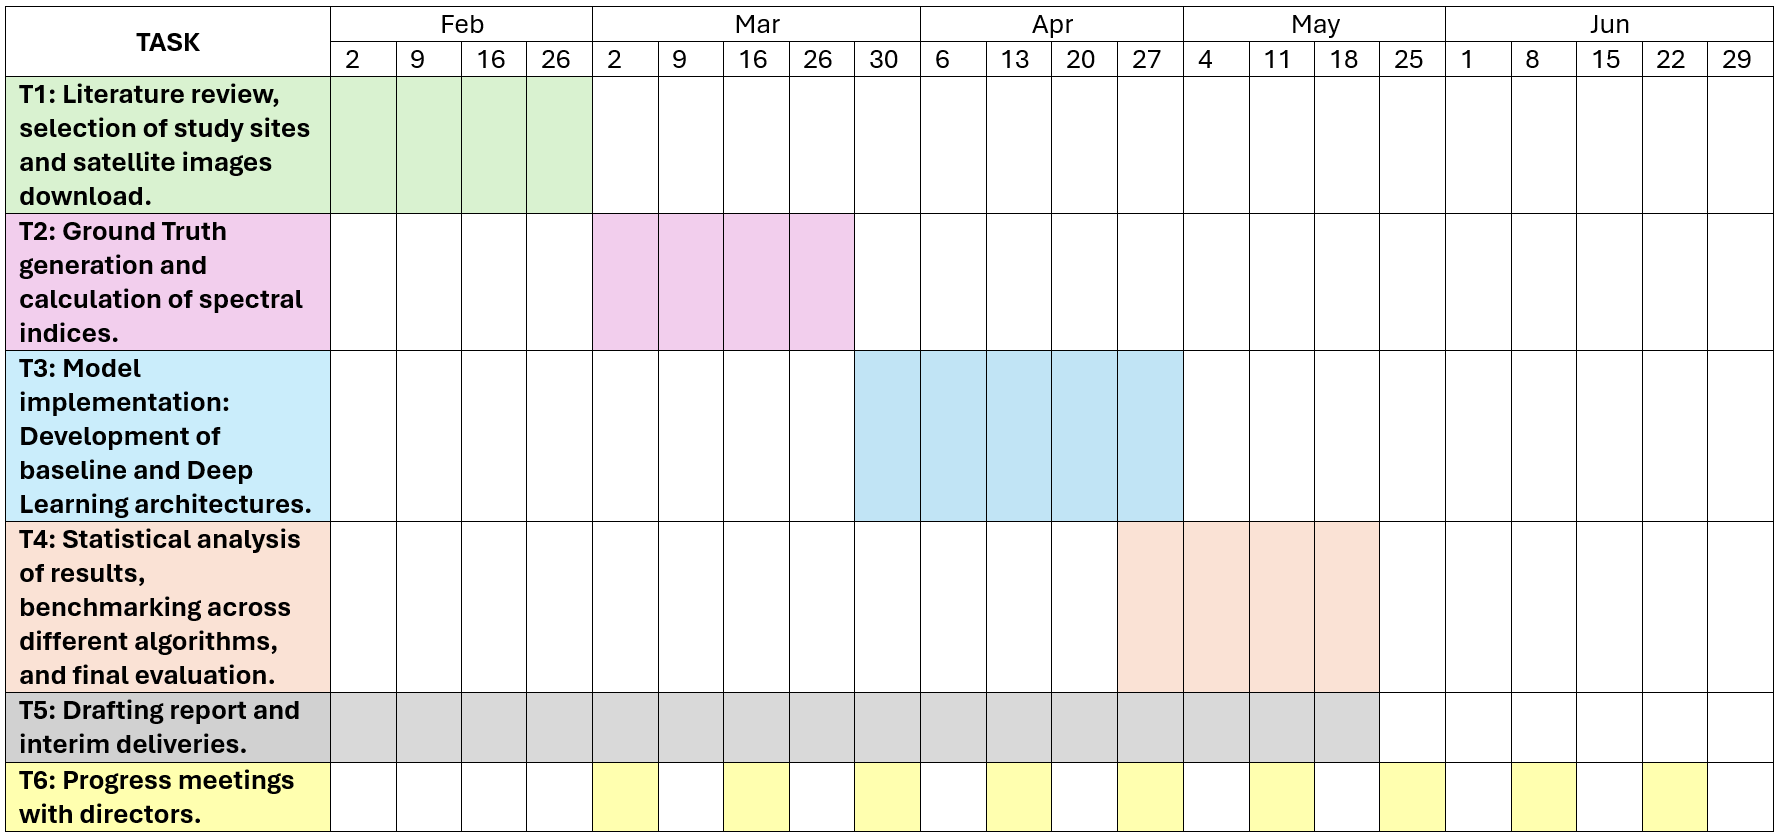
\includegraphics[width=15truecm]{tfm_gantt.png}
    \caption{Gantt chart of the project timeline.}
    \label{fig:gantt}
\end{figure}

\section{Brief Summary of Products Obtained}

TO BE WRITTEN

\section{Brief Description of Other Memory Chapters}

TO BE WRITTEN

\section{Statement on the Use of Generative Artificial Intelligence}

TO BE WRITTEN

\chapter{State of Art}

\section{Coastal Monitoring and Shoreline Definition}

The analysis of shoreline evolution over time is a fundamental aspect of coastal science, engineering, and management. An idealized definition of the shoreline describes it as the physical interface between land and water \citep{boak_shoreline_2005}. However, this boundary is highly dynamic, driven by continuous fluctuations in water levels caused by tides, waves, storm surges, and seasonal changes. Consequently, capturing a single, definitive shoreline position is practically impossible, making it necessary to define the shoreline based on specific objectives and available data.

To overcome this, researchers typically rely on \textit{shoreline indicators}, which serve as proxy features to represent the true shoreline position. According to the comprehensive review by \citet{boak_shoreline_2005}, these indicators are generally grouped into two main categories:

\begin{itemize}
    \item \textbf{Visually discernible features}: Physical marks left on the coast, such as the High-Water Line (HWL) (often identified by a change in sand color due to moisture content), the instantaneous wet/dry boundary left by wave runup, or the seaward edge of dune vegetation (Figure \ref{fig:schematic_shoreline_indicators}).
    \item \textbf{Tidal datum-based indicators}: These define the shoreline as the intersection of a specific coastal profile with a predetermined vertical elevation, such as Mean High Water (MHW) or Mean Sea Level (MSL). While datum-based indicators provide a mathematically objective boundary, they often require high-resolution topographic data (e.g., DGPS or LiDAR) which can be hard to acquire for long-term or large-scale studies (Figure \ref{fig:schematic_shoreline_indicators}).
\end{itemize}

\begin{figure}[H]
    \centering
    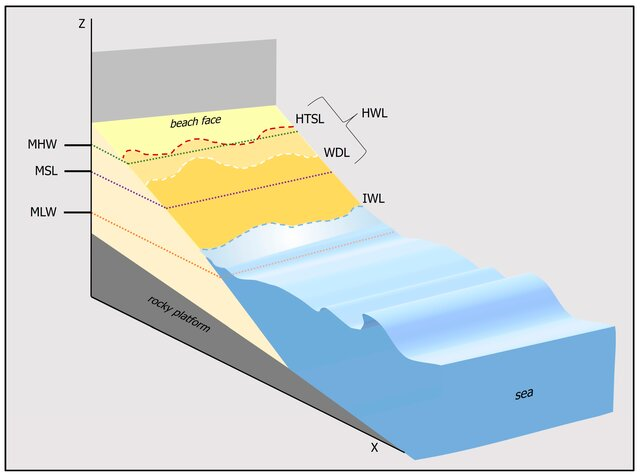
\includegraphics[width=12truecm]{Schematic-representation-of-Conceicao-Duquesa-beach-profile-illustrating-shoreline_W640.jpg}
    \caption{Schematic representation of a beach profile illustrating shoreline indicators.(1) Feature based, detected on beach face: HTSL—high-tide swash line; WDL—wet–dry line; HWL—high-water line; IWL—instantaneous water line. (2) Elevation-based: MHW—mean high-water, MSL—mean sea level; MLW—mean low-water. (Source: \citealp{valverde_historical_2025})}
    \label{fig:schematic_shoreline_indicators}
\end{figure}

The selection of a specific indicator and monitoring frequency depends on the intended application of the data. Shoreline monitoring serves several critical functions:
\begin{itemize}
    \item \textit{Long-term Trend Analysis}: Quantifying multi-decadal erosion or accretion rates to understand coastline evolution.
    \item \textit{Storm Impact Assessment}: Evaluating episodic erosion caused by extreme weather events and tracking the subsequent post-storm recovery.
    \item \textit{Seasonal Variability Studies}: Capturing the cyclical movement of the shoreline due to changing wave climates between summer and winter.
    \item \textit{Coastal Management}: Quantifying the dry beach width for coastal management purposes, such as evaluating the beach's natural potential to act as a coastal defense against storms, assessing its carrying capacity for tourism and recreational activities, and informing strategies to mitigate overall vulnerability.
\end{itemize}

Within this theoretical framework, it is essential to define the specific indicator addressed in this research. This Master's Thesis focuses exclusively on the instantaneous waterline (WL), defined as the precise boundary between the water body and the emerged land at the exact moment of satellite overpass. While the term \textit{shoreline} is often used in a broader sense in coastal literature, throughout this document, both \textit{shoreline} and \textit{waterline} (or the acronym SDW for Satellite-Derived Waterline) are used interchangeably to refer specifically to this instantaneous land-water interface. Focusing on the WL is particularly relevant for satellite-based monitoring, as it represents the most direct feature discernible from optical imagery, although its detection in macrotidal environments remains a significant technical challenge, as will be described in more detail in Section \ref{sec:soa_challenges_macrotidal}.

\section{Traditional Coastal Monitoring Methods}

Historically, coastal monitoring has relied heavily on in-situ physical surveys. While these methods can offer high precision, they are inherently constrained by significant logistical effort, high operational costs, and consequently, low spatial and temporal coverage. 

Topobathymetric monitoring using Global Navigation Satellite Systems (GNSS), particularly those operating in Real-Time Kinematic (RTK) mode, have been widely employed to acquire cross-shore beach profiles \citep{morton_monitoring_1993}. Although GNSS-based techniques can achieve millimeter-level accuracy, data collection is limited to the physical path traversed by operators (e.g., walking, driving, or mounted on a vehicle), making continuous shoreline mapping over regional scales largely impractical.

To bridge the spatial gap of ground surveys, researchers increasingly turned to advanced airborne scanning technologies such as Light Detection and Ranging (LiDAR). Airborne LiDAR allows for the rapid acquisition of dense, high-resolution 3D point clouds over hundreds of kilometers of coast, from which datum-based shorelines can be extracted objectively \citep{stockdon_estimation_2002}. However, the high economic cost of instrument deployment restricts its use to infrequent, opportunistic, or project-specific flights, failing to provide the high-frequency temporal data necessary for continuous monitoring.

Addressing the temporal limitations of physical surveys, fixed coastal video monitoring systems (most notably the Argus system \citep{holman_application_1993}) were developed in the 1990s. These ground-based camera networks capture high-frequency images (e.g., every 10 minutes) and can produce time-averaged images to derive robust shoreline-proxy indicators. While providing excellent temporal resolution to track short-term morphological changes, their spatial coverage remains inextricably confined to the camera's visual field of view (typically 1–3 kilometers), leaving vast stretches of the coastline unmonitored.

More recently, the rise of ubiquitous smartphone technology has catalyzed the development of Citizen Science approaches for coastal monitoring, best exemplified by the global CoastSnap project \citep{harley_coastsnap_2022}. By installing simple, low-cost smartphone cradles at strategic coastal viewpoints, these initiatives crowdsource beach imagery from the general public. While this drastically reduces both initial deployment and operational costs while providing data with a spatial resolution similar to video stations, the temporal frequency and reliability of the data are inherently opportunistic, depending entirely on community participation and favorable weather conditions.

To overcome the inherent trade-offs between spatial coverage, temporal frequency, and operational costs present in these traditional methods, researchers have increasingly turned to Earth Observation (EO) satellites. As summarized in Table \ref{tab:monitoring_methods}, satellite imagery uniquely provides continuous, global-scale coverage with a high frequency of observations at virtually zero operational cost for the end-user, effectively resolving many of the historical monitoring limitations. The application of this remote sensing data for continuous shoreline extraction, which is the cornerstone of this thesis, will be discussed in detail in the following section (Section \ref{sec:soa_satellite_methods}).

\begin{table}[H]
    \centering
    \caption{Summary of common coastal monitoring methods and their key characteristics.}
    \vspace{0.1cm}
    \renewcommand{\arraystretch}{1.5}
    \resizebox{\textwidth}{!}{
    \begin{tabular}{l c c c l}
        \hline
        \textbf{Monitoring Method} & \textbf{Spatial Scale} & \textbf{Spatial Resolution} & \textbf{Temporal Resolution} & \textbf{Operational Cost} \\
        \hline
        GNSS / RTK Topography & Local & Millimetric & Low (Infrequent) & Very High (per survey) \\
        Airborne LiDAR & Regional & Sub-meter & Low (Infrequent) & Very High (per flight) \\
        Video systems (Argus) & Local (1-3 km)& Centimetric & Very High (Minutes) & Low (after initial setup) \\
        Citizen Science (CoastSnap) & Local & Centimetric & Highly Variable & Very Low \\
        Optical satellites (i.e. Landsat 4-9 and Sentinel-2) & Global & Decametric (10 m) & High (Days) & Zero (Free open data) \\
        \hline
    \end{tabular}
    }
    \label{tab:monitoring_methods}
\end{table}

\section{Satellite Remote Sensing for Coastal Monitoring} \label{sec:soa_satellite_methods}

The advent of Earth Observation (EO) satellites has profoundly democratized and revolutionized coastal monitoring, effectively resolving the historical trade-offs between spatial coverage and temporal frequency. The cornerstone of this revolution is the Landsat program, jointly managed by NASA and the USGS. Initiated in the 1970s and providing continuous 30-meter resolution optical imagery since the launch of Landsat 4 in 1982, it offers an unparalleled, retrospective archive spanning over four decades. This extensive catalog allows coastal scientists and managers to reconstruct long-term shoreline evolution, analyze multi-decadal erosion trends, and assess the historical impact of major climatic events on a truly global scale.

Building upon this legacy, the European Space Agency (ESA) catalyzed a new era in EO with the launch of the Copernicus Sentinel-2 constellation. Initially a twin-satellite system (Sentinel-2A and 2B, launched in 2015 and 2017), the constellation has recently been reinforced with the launch of Sentinel-2C in September 2024. Sentinel-2 dramatically bridged the gap to traditional in-situ methods by providing freely available, multispectral imagery at an unprecedented 10-meter spatial resolution (in visible and Near-Infrared bands) with a high-frequency revisit time of just 5 days at the equator \citep{vitousek_future_2023}. This exponential leap in temporal resolution has unlocked the ability to monitor highly dynamic, short-term coastal processes from space, such as seasonal beach profile fluctuations (e.g., \citealp{warrick_shoreline_2025}) and the acute morphodynamic impacts of specific storms (e.g., \citealp{cabezas-rabadan_satellite_2024}). The synergistic combination of both Landsat and Sentinel-2 missions has sparked an exponential growth in satellite-derived shoreline research over the last decade (Figure \ref{fig:evolution_shoreline_satellite}).

\begin{figure}[H]
    \centering
    \textbf{(a)}\par\medskip
    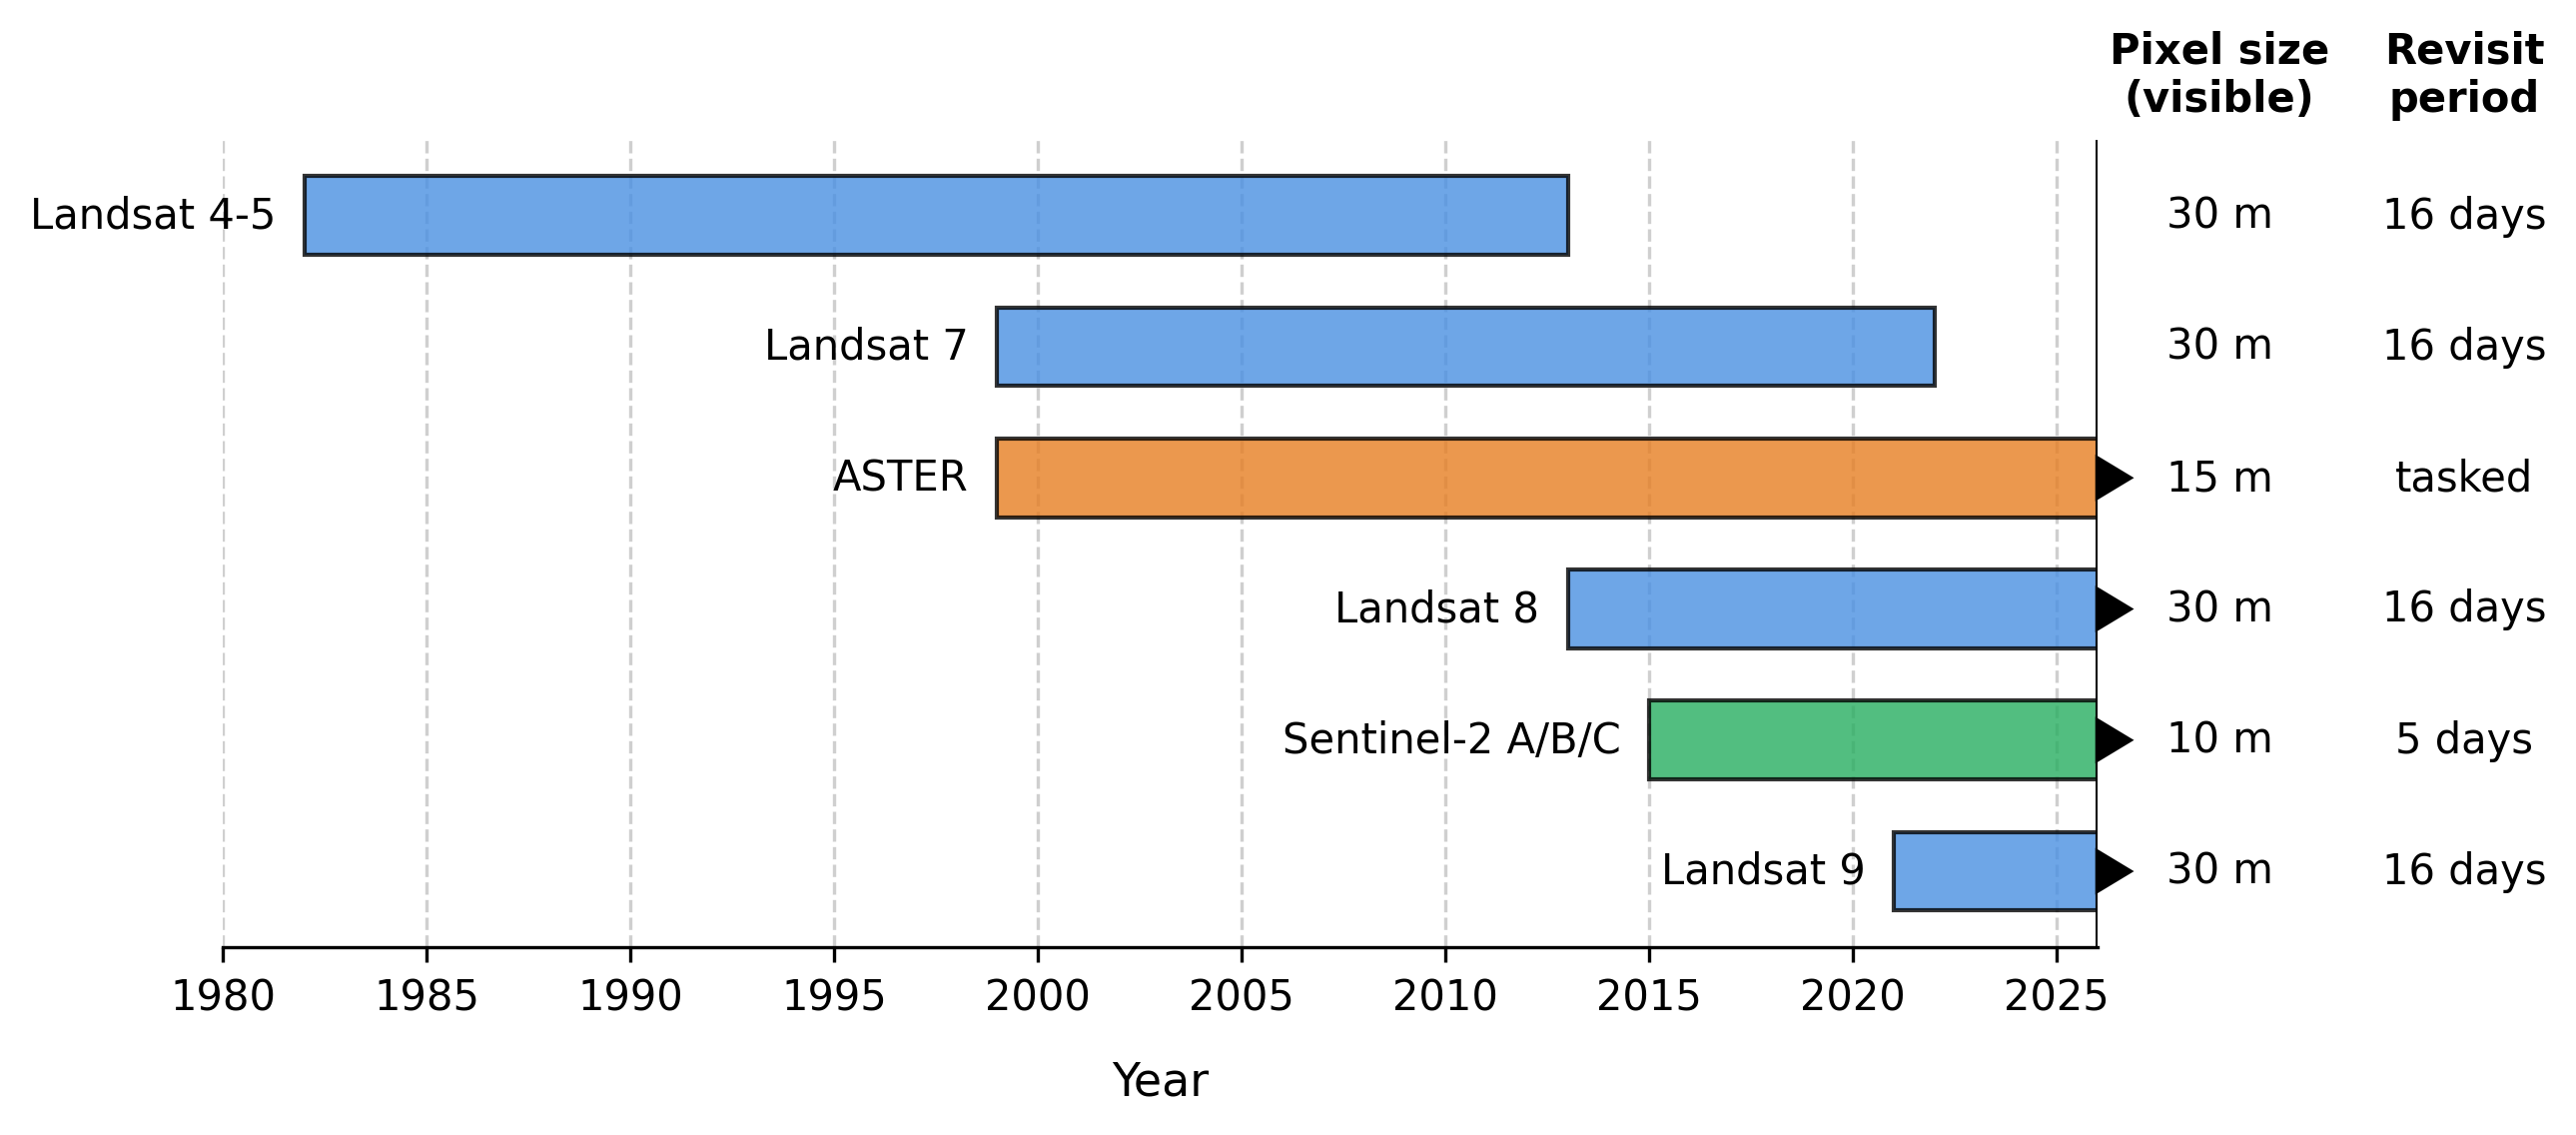
\includegraphics[width=15truecm]{satellite_timeline.png}
    \vspace{0.05cm}
    
    \textbf{(b)}\par\medskip
    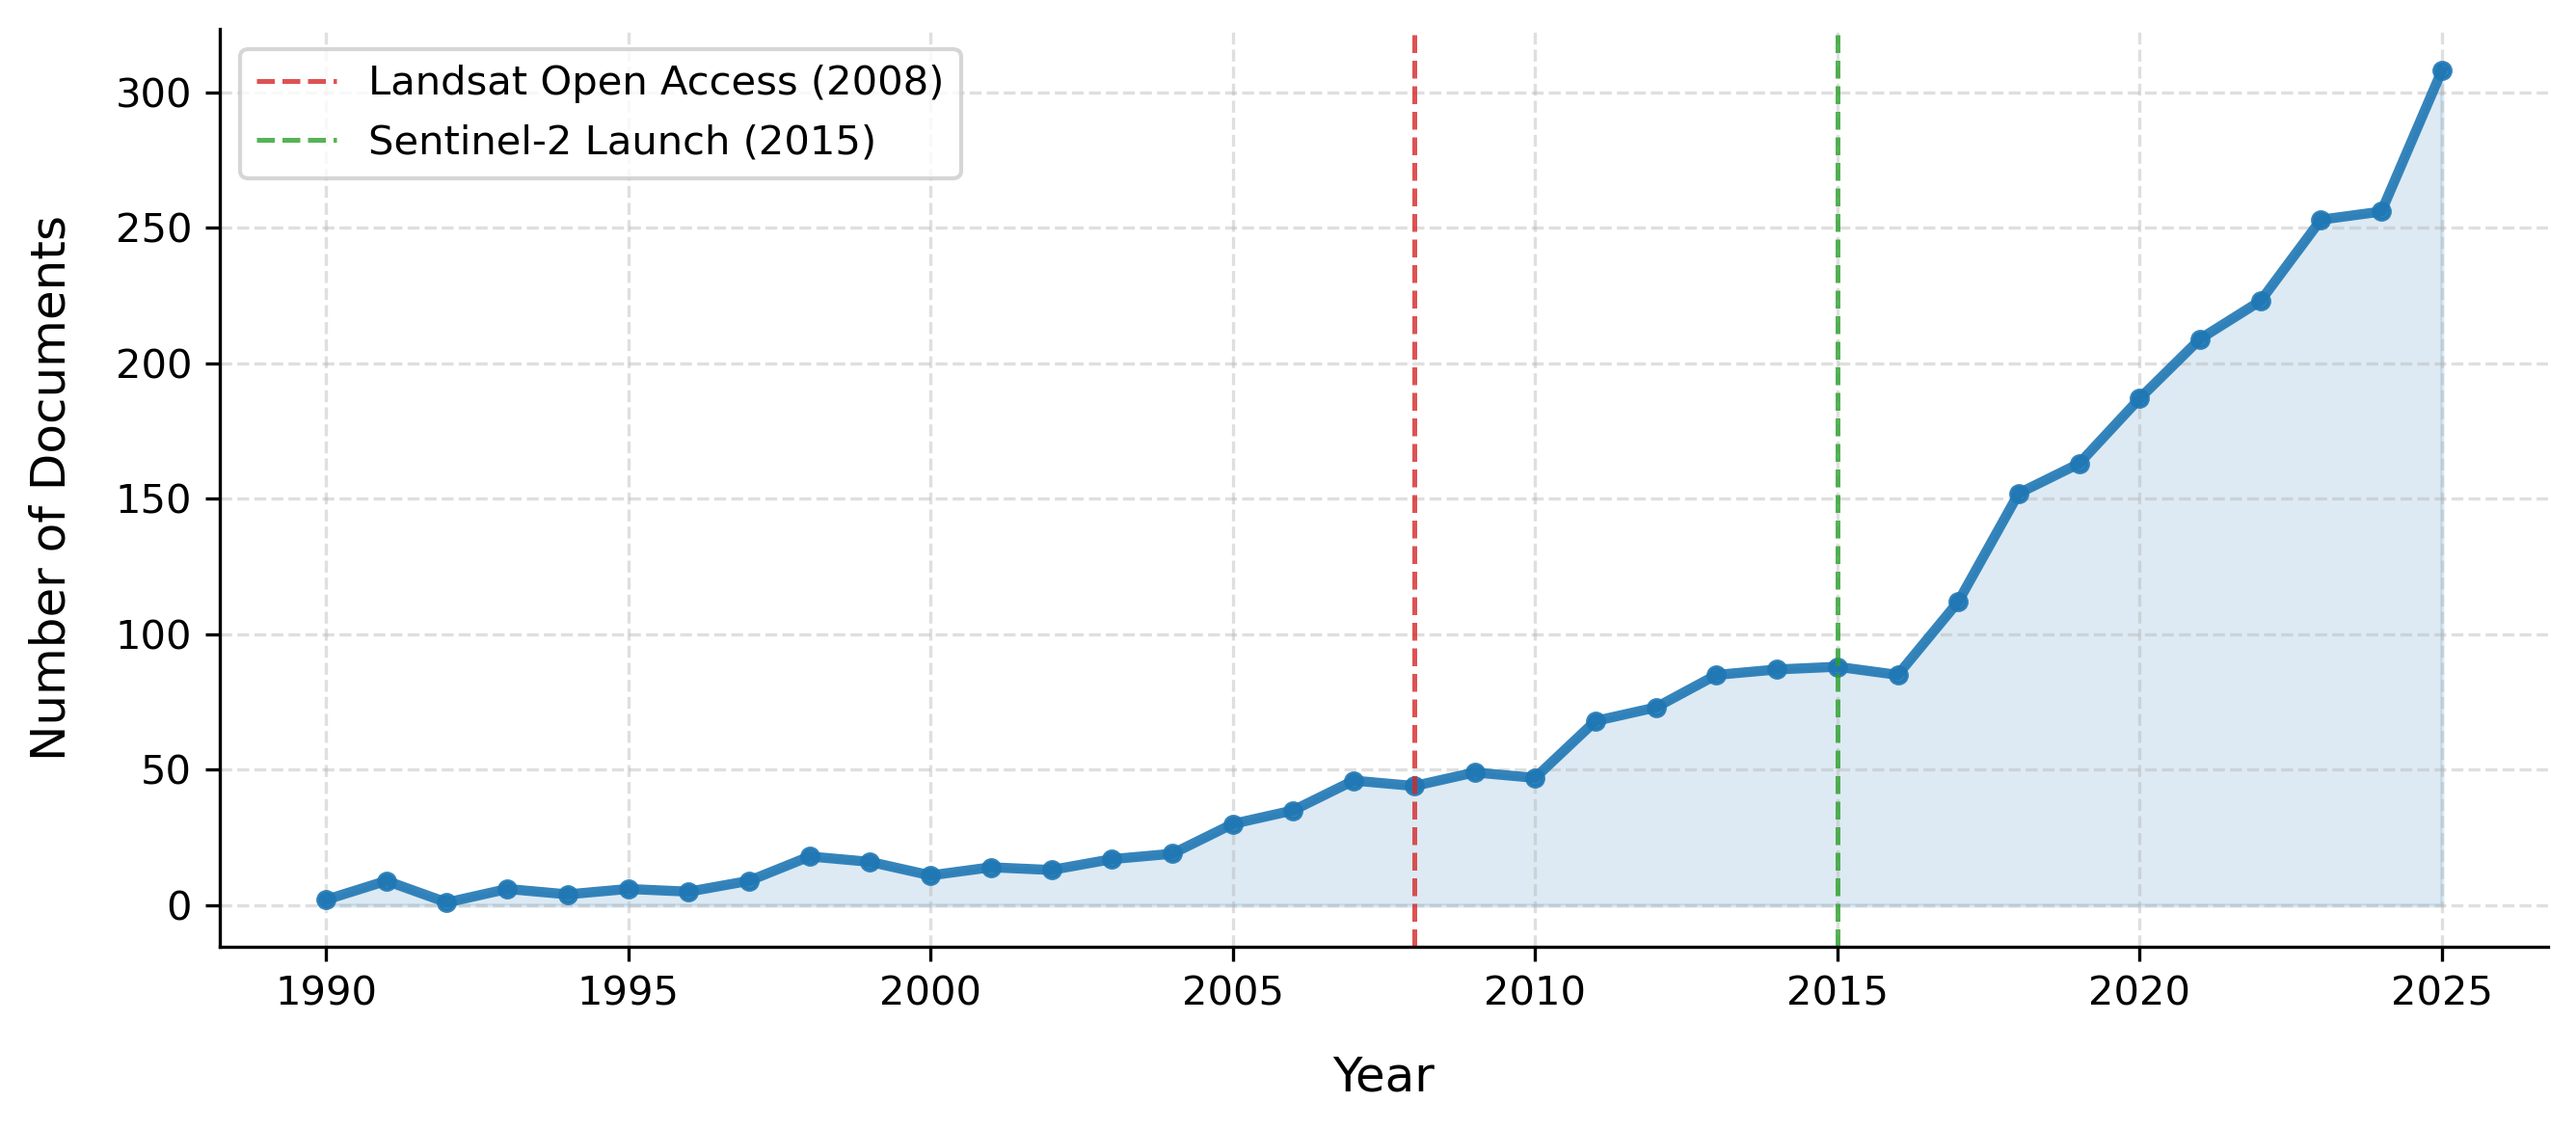
\includegraphics[width=15truecm]{evolution_shoreline_satellite.png}
    \caption{(a) Timeline for the publicly available satellites with global coverage. Source: Own elaboration, adapted and updated from \citet{vos_sub-annual_2019}. (b) Rapid evolution of the number of publications on satellite-derived shorelines (Number of documents per year for documents that include keywords ``satellite'' AND ``shoreline'' in Scopus database).}
    \label{fig:evolution_shoreline_satellite}
\end{figure}

To leverage this massive and continuously expanding volume of ``Big Data'', the scientific community recognized that manual shoreline delineation was virtually impossible. This necessitated the development of automated computational frameworks designed to extract shoreline positions efficiently. Notable examples include CoastSat \citep{vos_coastsat_2019}, CASSIE \citep{almeida_coastal_2021}, and SHOREX \citep{sanchez-garcia_efficient_2020}. While differing in their specific implementations, these tools generally share a common processing pipeline: automated image acquisition via cloud APIs (like Google Earth Engine), cloud and cloud-shadow masking, initial water/land segmentation at the pixel level using spectral indices, and finally, subpixel contouring techniques to delineate the final, continuous shoreline vector. 

\section{Traditional Waterline Extraction via Spectral Indices}

The critical step in traditional SDW extraction pipelines is the initial segmentation of the image into ``water'' and ``non-water'' classes. This is almost universally achieved using Spectral Water Indices. These indices exploit the characteristic of water to absorb most radiation in the Near-Infrared (NIR) and Shortwave-Infrared (SWIR) wavelengths, while land (soil, sand, and vegetation) strongly reflects them (see Figure~\ref{fig:spectral_indices}).

\begin{figure}[H]
    \centering
    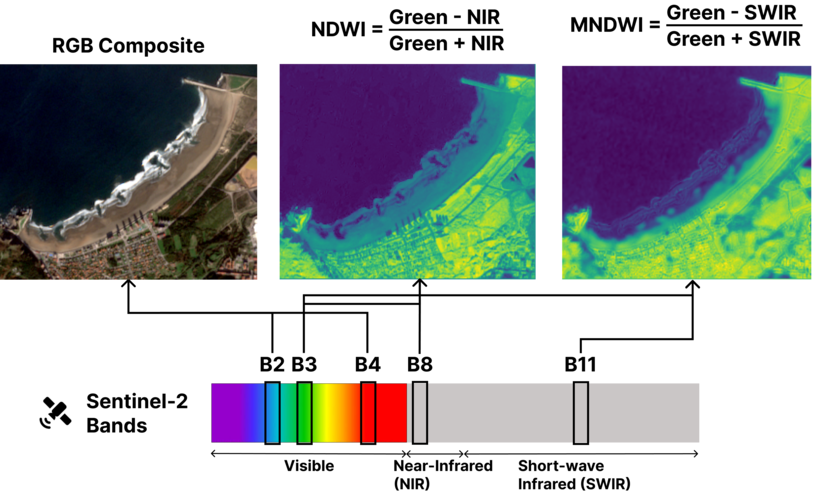
\includegraphics[width=12truecm]{figure_intro_spectral_indices.png}
    \caption{Schematic diagram of spectral index calculations using Sentinel-2 bands.}
    \label{fig:spectral_indices}
\end{figure}

Historically, the Normalized Difference Water Index (NDWI), proposed by \citet{mcfeeters_use_1996}, and its variant, the Modified Normalized Difference Water Index (MNDWI) introduced by \citet{xu_modification_2006}, have been the standard tools for this task. Their implementation has been extensively documented in scientific literature to track long-term shoreline evolution and morphological changes across diverse coastal settings. For instance \citet{ghosh_monitoring_2015}, \citet{liu_analysis_2017} or \citet{wang_spatio-temporal_2017} demonstrated the efficacy of these indices in achieving high-accuracy shoreline detection using medium resolution satellite imagery, proving their value for multi-decadal coastal monitoring.

More recently, indices designed specifically to suppress environmental noise and improve performance in complex coastal scenes have been introduced. These include the Automated Water Extraction Index (AWEI), developed by \citet{feyisa_automated_2014} to enhance water shadows and urban background removal, and the Subtractive Coastal Water Index (SCoWI) \citep{bergsma_shoreliner_2024}. The latter is particularly relevant to this project as it was developed specifically for Sentinel-2 imagery and has shown promising results in macrotidal environments.

Once the index is calculated to create a greyscale intensity map, a threshold must be applied to binarize the image. While setting a constant threshold (e.g., zero) is common, adaptive statistical methods like Otsu's thresholding (\citealp{otsu_threshold_1979}) are frequently used to find the optimal separation value based on the image's histogram distribution. After binarization, the shoreline is extracted by identifying the boundary between water and land pixels. This is typically done by finding the transition pixels between the two classes, which are then smoothed and converted into a vector line via subpixel contouring algorithms (such as marching-squares, \citealp{lorensen_marching_1987}).

\section{Challenges and Limitations in Macrotidal Environments} \label{sec:soa_challenges_macrotidal}

While traditional spectral indices combined with automated thresholding (e.g., Otsu) perform highly accurately (often achieving sub-pixel precision of $<$10~m) in microtidal, sheltered, or steeply sloped beaches, their reliability significantly degrades in complex, high-energy, and macrotidal environments. Recent global benchmarking efforts \citep{vos_benchmarking_2023} have quantified this degradation, showing that horizontal extraction errors more than double (exceeding 20-40~m) on macrotidal beaches compared to their microtidal counterparts. Furthermore, site-specific assessments across the European Atlantic coast have similarly revealed profound limitations in these segmentation techniques during challenging oceanographic conditions \citep{cabezas_site-specific_2026}.

The primary driver of error in these settings is the extensive and topographically complex intertidal zone exposed during ebb and low tides. In macrotidal beaches (tidal ranges $>$ 4 m) characterized by intermediate or dissipative morphodynamic states, the retreating tide leaves behind vast plains of saturated sand. Spectrally, the transition from dry sand to wet sand to shallow water is not a sharp boundary but a gradual continuum. Indices such as MNDWI and AWEInsh consistently fail to differentiate between shallow water and saturated soil, systematically misclassifying the wet intertidal zone as ``water'' (see an example in Figure \ref{fig:mndwi_cross_section}). This results in the extraction algorithms delineating the upper limit of the wet beach (or even the dune vegetation line) rather than the instantaneous water level, creating massive landward biases that can exceed hundreds of meters.

\begin{figure}[H]
    \centering
    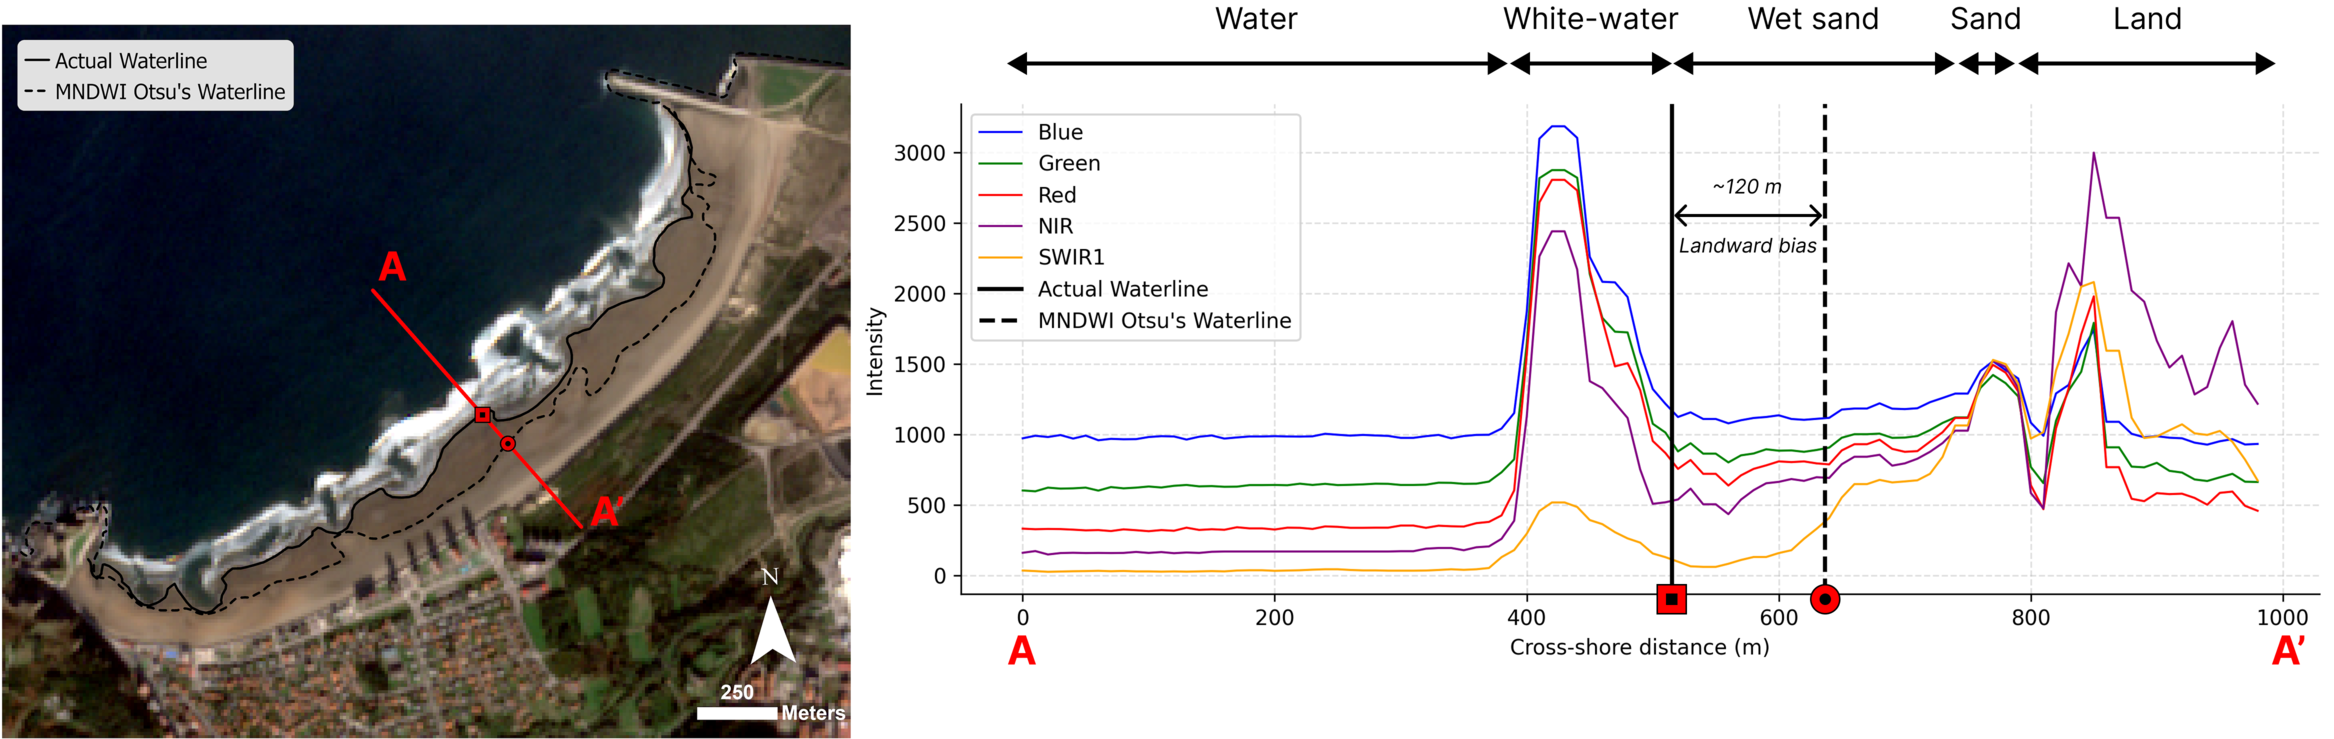
\includegraphics[width=17truecm]{mndwi_cross_section.png}
    \caption{Cross-section of a macrotidal beach showing the spectral signature of water, white-water, wet sand, sand and land, derived from a Sentinel-2 image. The dashed line represents the shoreline extracted using MNDWI and Otsu's thresholding method, whereas the solid line represents the actual waterline. The MNDWI index is not able to differentiate between wet sand and water, leading to a landward bias in the extracted shoreline up to 120 m.}
    \label{fig:mndwi_cross_section}
\end{figure}

Furthermore, high-energy wave conditions may introduce additional errors. The presence of extensive white foam generated by breaking waves offshore drastically alters the expected low reflectance of the water surface. Indices like NDWI are particularly sensitive to foam, occasionally mistaking the outer breaker zone for land, thus producing severe seaward offsets \citep{hagenaars_accuracy_2018, cabezas_site-specific_2026}.

Ultimately, both specific case studies \citep{cabezas_site-specific_2026} and comprehensive benchmarking exercises \citep{vos_benchmarking_2023} concur that the primary bottleneck for accurate SDW extraction in complex areas is not the geometric subpixel refinement algorithm, but the initial binary segmentation step (the spectral index determination and thresholding method) itself. Relying solely on the radiometric intensity of isolated pixels is insufficient to navigate the semantic ambiguity between wave foam, wet sand, and the actual waterline. This critical limitation strongly motivates the need to take a step back from classical spectral approaches and explore advanced, context-aware Deep Learning solutions.

\section{The Shift towards Deep Learning in Earth Observation}

To overcome the inherent limitations of pixel-by-pixel spectral thresholding, the remote sensing community is increasingly turning to Deep Learning (DL). Unlike traditional index thresholds that evaluate the reflectance value of an isolated pixel, advanced DL semantic segmentation architectures learn hierarchical spatial features by evaluating the spatial context, textures, and structural patterns. This contextual awareness allows models to distinguish the texture of wave foam from dry sand or recognize the spatial gradient of a saturated beach face, even when spectral signatures are nearly identical.

While the field is rapidly evolving, the technical landscape of DL for coastal monitoring is characterized by several competing paradigms. The encoder-decoder framework, exemplified by U-Net \citep{navab_u-net_2015} and its variants, remains the most prevalent architecture due to its effective use of skip connections to preserve fine spatial details \citep{tsiakos_use_2023}. More advanced convolutional models, such as DeepLabV3+ \citep{chen_encoder-decoder_2018}, have shown great potential by explicitly evaluating the image at multiple scales simultaneously. This wider field of view allows the model to better understand the broader coastal context (like the general geometry of the beach) while focusing sharply on the exact boundary, making it highly beneficial for extracting continuous, uninterrupted waterlines even in complex coasts.

Furthermore, a significant shift toward Vision Transformers (ViT) and hybrid architectures is underway. Models like SegFormer \citep{xie_segformer_2021} and SETR \citep{zheng_rethinking_2020} demonstrate a superior ability to incorporate global contextual information, which is critical for distinguishing water boundaries in scenes affected by intense wave splash and structural shadows. More recently, dual-branch architectures such as TCCFNet \citep{fu_tccfnet_2025} have emerged as highly synergistic networks, combining CNN layers for fine, local details with Transformer layers for large-scale scene understanding. Although TCCFNet was originally designed for mapping complex mangrove forests rather than strictly for shoreline extraction, its underlying mechanics are transferable to waterline mapping. By leveraging global context to understand the broader beach morphology while using local features to precisely trace the tricky land-water interface, this hybrid approach can drastically reduce the semantic confusion between visually similar elements like shallow water and wet sand. To push this focus on the transition zone even further, specialized boundary-aware networks (such as BS-Net \citep{jing_bs-net_2021} and BAWS \citep{zhan_usv-seg_2025}) have been developed to treat the land-water interface as a primary feature rather than just the edge of a mask. By assigning dedicated interaction modules to explicitly model the boundary itself, these networks guarantee the high metric precision necessary for operational coastal monitoring.

Despite these architectural advancements, a critical analysis of the current state of the art reveals fundamental methodological gaps that this study aims to address:

\begin{itemize}
    \item \textbf{Transition from Basic ML to Deep Contextual Learning:} While earlier AI applications for shoreline extraction heavily relied on traditional, pixel-wise Machine Learning classifiers (such as Support Vector Machines, Random Forests, or K-Nearest Neighbors), these methods still struggle with the complex spectral mixtures found in dynamic coastal zones \citep{tsiakos_use_2023}. Modern Deep Learning architectures overcome this by evaluating the spatial context rather than isolated pixels, though their full potential in adverse conditions is yet to be systematically quantified.
    
    \item \textbf{The Macrotidal Gap:} Most DL studies for shoreline extraction have been trained and validated in microtidal or sheltered environments where the land-water boundary is relatively stable. In macrotidal coasts, the ``semantic ambiguity'' between breaking wave foam, saturated sand, and shallow water remains a systematic challenge that most current models treat as noise rather than learned features \citep{tian_deep_2024}. The effectiveness of DL models to navigate these specific, high-energy conditions is a critical void in current research.

    \item \textbf{Lack of Systematic Benchmarking vs. Operational Spectral Tools:} Although tools like CoastSat, CASSIE or SHOREX (which rely on spectral indices and automatic thresholding) are the current operational standard for automated shoreline extraction, there is a striking absence of extensive, consistent benchmarking that formally compares these traditional pipelines against modern semantic segmentation models \citep{tian_deep_2024}. Most DL studies evaluate new architectures against other neural networks rather than quantifying the exact magnitude of improvement over index-based methods in challenging environments.
    
    \item \textbf{Architectural Over-reliance and Class Complexity}: Current literature shows an over-reliance on U-Net variants without systematic justification for more complex coastal scenes \citep{tian_deep_2024}. Furthermore, most models still approach the problem as a binary classification (water vs. land), failing to exploit the potential of multi-class segmentation (e.g., explicitly labeling ``wet sand'' or ``white water'') to reduce the confusion that leads to landward or seaward biases.

\end{itemize}

By presenting a direct, data-driven comparison of classical spectral thresholding and modern semantic segmentation models (specifically optimized for multi-class detection in macrotidal settings), this project directly targets these gaps. It seeks not only to improve accuracy but to provide a rigorous assessment of whether AI-based workflows offer a justifiable operational advantage over established index-based monitoring tools.

\chapter{Materials and Methods}

This chapter details the comprehensive methodological framework developed to evaluate and benchmark the performance of traditional spectral methods against Deep Learning semantic segmentation models for macrotidal waterline extraction. To provide a clear roadmap of the research, Figure \ref{fig:ch3_workflow} illustrates the end-to-end processing pipeline. The workflow encompasses five primary stages: the definition of the study areas (Section \ref{sec:study_areas}); the acquisition and preprocessing of satellite and oceanographic data (Section \ref{sec:data_acquisition}); the generation of Ground Truth reference datasets (Section \ref{sec:ground_truth}); the implementation of both traditional and AI-based extraction pipelines (Sections \ref{sec:baseline_spectral} to \ref{sec:waterline_pipeline}); and finally, the pixel-based and geometric evaluation methodologies (Section \ref{sec:evaluation_methodology}).

\begin{figure}[H]
    \centering
    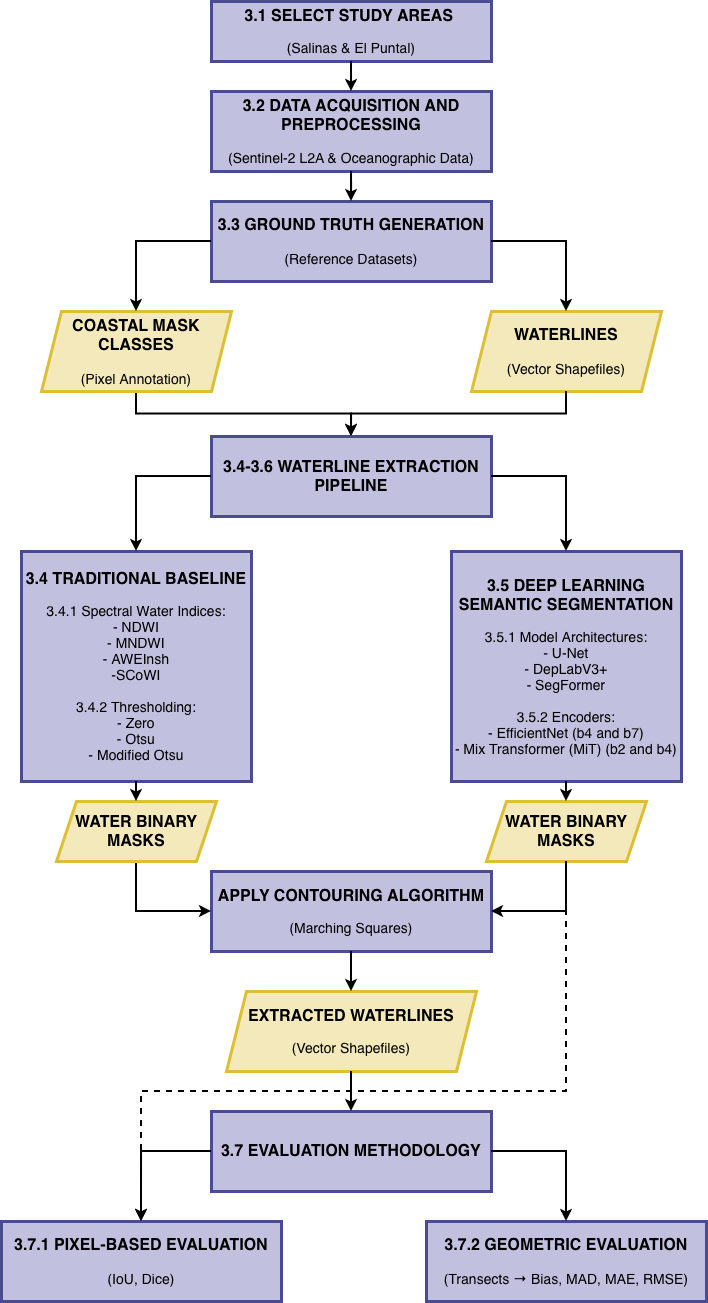
\includegraphics[scale=0.43]{diagram_methodology.png}
    \caption{General methodological workflow of the study. The diagram outlines the data acquisition, model training, extraction pipelines, and evaluation stages detailed throughout this chapter.}
    \label{fig:ch3_workflow}
\end{figure}

\section{Study Areas}
\label{sec:study_areas}

The study focuses on two beaches located on the northern coast of Spain: Salinas (Asturias) and El Puntal (Cantabria) (Figure \ref{fig:study_sites}).

Salinas is a 2.5 km embayed sandy beach system located on the left bank of the Avilés estuarine inlet (Asturias). The beach is bounded by an inlet jetty to the east and a rocky headland (La Peñona) to the west. Its western sector, adjacent to the urban area of Salinas, is backed by a seawall and promenade, while the eastern sector (El Espartal) preserves a natural dune field rising up to 15 m above mean sea level. The beach is characterized by a wide intertidal zone (up to 300 m at spring tides) and a mean tidal range of 4.5 m, classifying it as a macrotidal environment. The wave climate is predominantly energetic and approach from the northwest, impacting directly with mean significant wave heights around 1 m and frequent storm events that can exceed 4 m. The sand often shows dark patches due to the accumulation of coal and carbonaceous shales, which can further complicate spectral differentiation between wet sand and water.

El Puntal is a 4 km sandy spit at the entrance of Santander Bay (Cantabria), formed by the interaction of estuarine and marine dynamics. The beach is backed by a dune system that reaches up to 10 m high and 50–100 m wide. The sandspit is located at its western end, whereas the eastern end is characterized by a more exposed morphology and the mouth of a small stream. In the same way as Salinas, El Puntal experiences a wide intertidal zone (up to 250 m) and a mean tidal range of around 4 m. However, unlike Salinas, El Puntal does not receive direct wave impact, as it is protected by the Magdalena Peninsula. Furthermore, also in contrast to Salinas, El Puntal features a much less dark, golden-colored sand.

\begin{figure}[H]
    \centering
    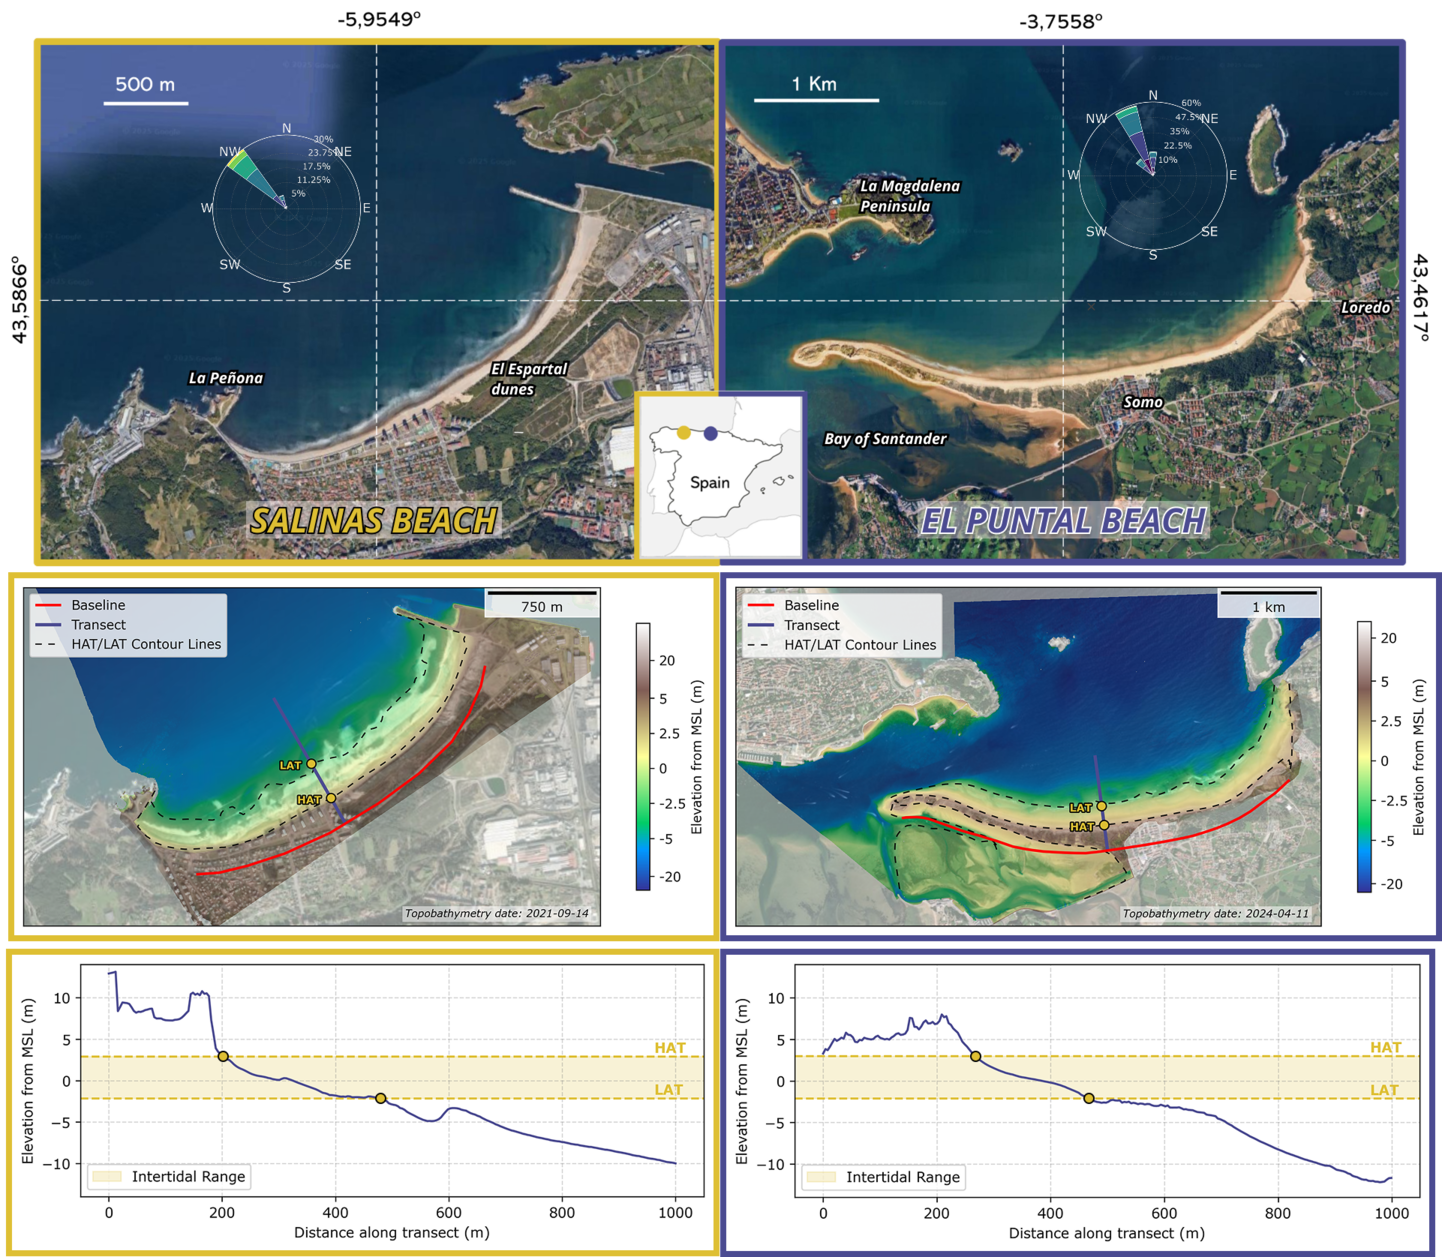
\includegraphics[width=15truecm]{Study_sites_figure.png}
    \caption{Location of the study sites: Salinas (left) and El Puntal (right) beaches. RGB image (top), topobathymetry (middle) using the ETRS89 / UTM 30N coordinate system, and beach profile (bottom) highlighting the intertidal range defined by the HAT/LAT (Highest/Lowest Astronomical Tide). (Source: \citealp{cabezas_site-specific_2026})}
    \label{fig:study_sites}
\end{figure}

The selection of Salinas and El Puntal as study areas responds to their representativeness of highly dynamic macrotidal environments, which consistently pose the most significant challenges for automated shoreline extraction methodologies. Both beaches share practically identical macrotidal ranges, featuring extensive intertidal zones that undergo profound daily fluctuations and result in the recurrent exposure of vast stretches of saturated sand. This inherently generates a critical spectral ambiguity between shallow water and wet sand, severely penalizing traditional pixel-by-pixel segmentation indices.

However, while they share this macrotidal nature, they exhibit key differences that allow for a comprehensive evaluation of the models under varying degrees of complexity. El Puntal, being sheltered from direct wave impact, serves as a baseline scenario with standard, golden-colored sand. Additionally, artificial dredging operations are routinely carried out at the very tip of El Puntal to maintain the required water depth for the navigation channel into the Bay of Santander. This dredging results in a much steeper beach slope in that specific area, which drastically reduces the extent of the intertidal zone, one of the main factors contributing to the reduced complexity of this environment. Summed to the other factors, this makes El Puntal a slightly less challenging environment compared to Salinas. In stark contrast, Salinas is fully exposed to energetic wave climates, resulting in a significantly higher presence of breaking wave foam (white-water) across a wide surf zone. Furthermore, the frequent accumulation of coal and carbonaceous shales along its intertidal profile creates noticeably dark patches of saturated sand. This stark color closely mimics the inherently low reflectance signature of water bodies in optical satellite imagery. Together, the excessive foam and the deceptively dark wet sand render Salinas an ideal stress-test. It provides a robust framework to critically evaluate whether Deep Learning architectures can successfully leverage spatial and structural context to differentiate the actual waterline, overcoming the limitations where traditional spectral methods typically fail.

\section{Data Acquisition and Preprocessing}
\label{sec:data_acquisition}

An initial dataset of freely available Sentinel-2 Level-2A imagery, spanning the period from 2015 to 2025, was acquired for both study areas. The imagery was downloaded using the Python API for the Google Earth Engine. To ensure optimal visibility of the coastal features, an initial visual filtering process was applied to download only cloud-free scenes.

From the available multispectral data, six specific bands were selected to provide the necessary radiometric information for both the derivation of spectral indices and the feature extraction in Deep Learning models: Red (B04), Green (B03), Blue (B02), Near-Infrared (B08), Shortwave-Infrared 1 (B11), and Shortwave-Infrared 2 (B12). 

Following the data acquisition, a dedicated preprocessing pipeline was implemented. First, the original massive satellite tiles were spatially cropped to strictly encompass the defined Regions of Interest (ROIs) for Salinas and El Puntal. Second, given that Sentinel-2 bands possess varying native spatial resolutions, spatial homogenization was required. The SWIR 1 and SWIR 2 bands, natively captured at a 20~m resolution, were resampled to match the 10~m spatial resolution of the visible and NIR bands. Finally, to prepare the dataset for the subsequent training phase of the Deep Learning semantic segmentation models (see Section \ref{sec:dl_models}), the preprocessed image ROIs were systematically divided into smaller patches of $128 \times 128$ pixels.

In addition to the optical imagery, historical oceanographic data provided by Puertos del Estado (https://www.puertos.es/) were acquired to accurately characterize the hydrodynamic conditions of each scene. Time-series records of sea level and wave climate were downloaded and temporally intersected to associate each Sentinel-2 image with its corresponding tide level and wave conditions at the exact moment of image acquisition. This comprehensive metadata association allows for the systematic evaluation and comparison of the extraction models' performance under varying oceanographic regimes. Furthermore, these associated tidal variables were directly utilized to perform a robust stratification of the dataset prior to the Deep Learning training phase, as detailed in Section \ref{sec:training_setup}.

However, it is crucial to acknowledge an inherent temporal sampling bias in the dataset stemming from the satellite's orbital mechanics. Sentinel-2 operates on a sun-synchronous orbit, ensuring it passes over the study sites at approximately the same local solar time (mid-morning). Because the local astronomical tide cycles are partially phase-locked with the solar day, this strict overpass schedule implies that the satellite systematically misses the absolute high waters of spring tides at this specific location. As illustrated in Figure \ref{fig:marine_data_comparison}, this results in a truncated tidal distribution where high tides are never captured. Conversely, the significant wave height ($H_s$) captured by the satellite generally preserves the overall statistical distribution of the full oceanic time-series, although extreme storm conditions remain underrepresented both due to their lower frequency and the fact that they are typically accompanied by heavy cloud cover, which filters them out during the optical image selection step.

\begin{figure}[H]
    \centering
    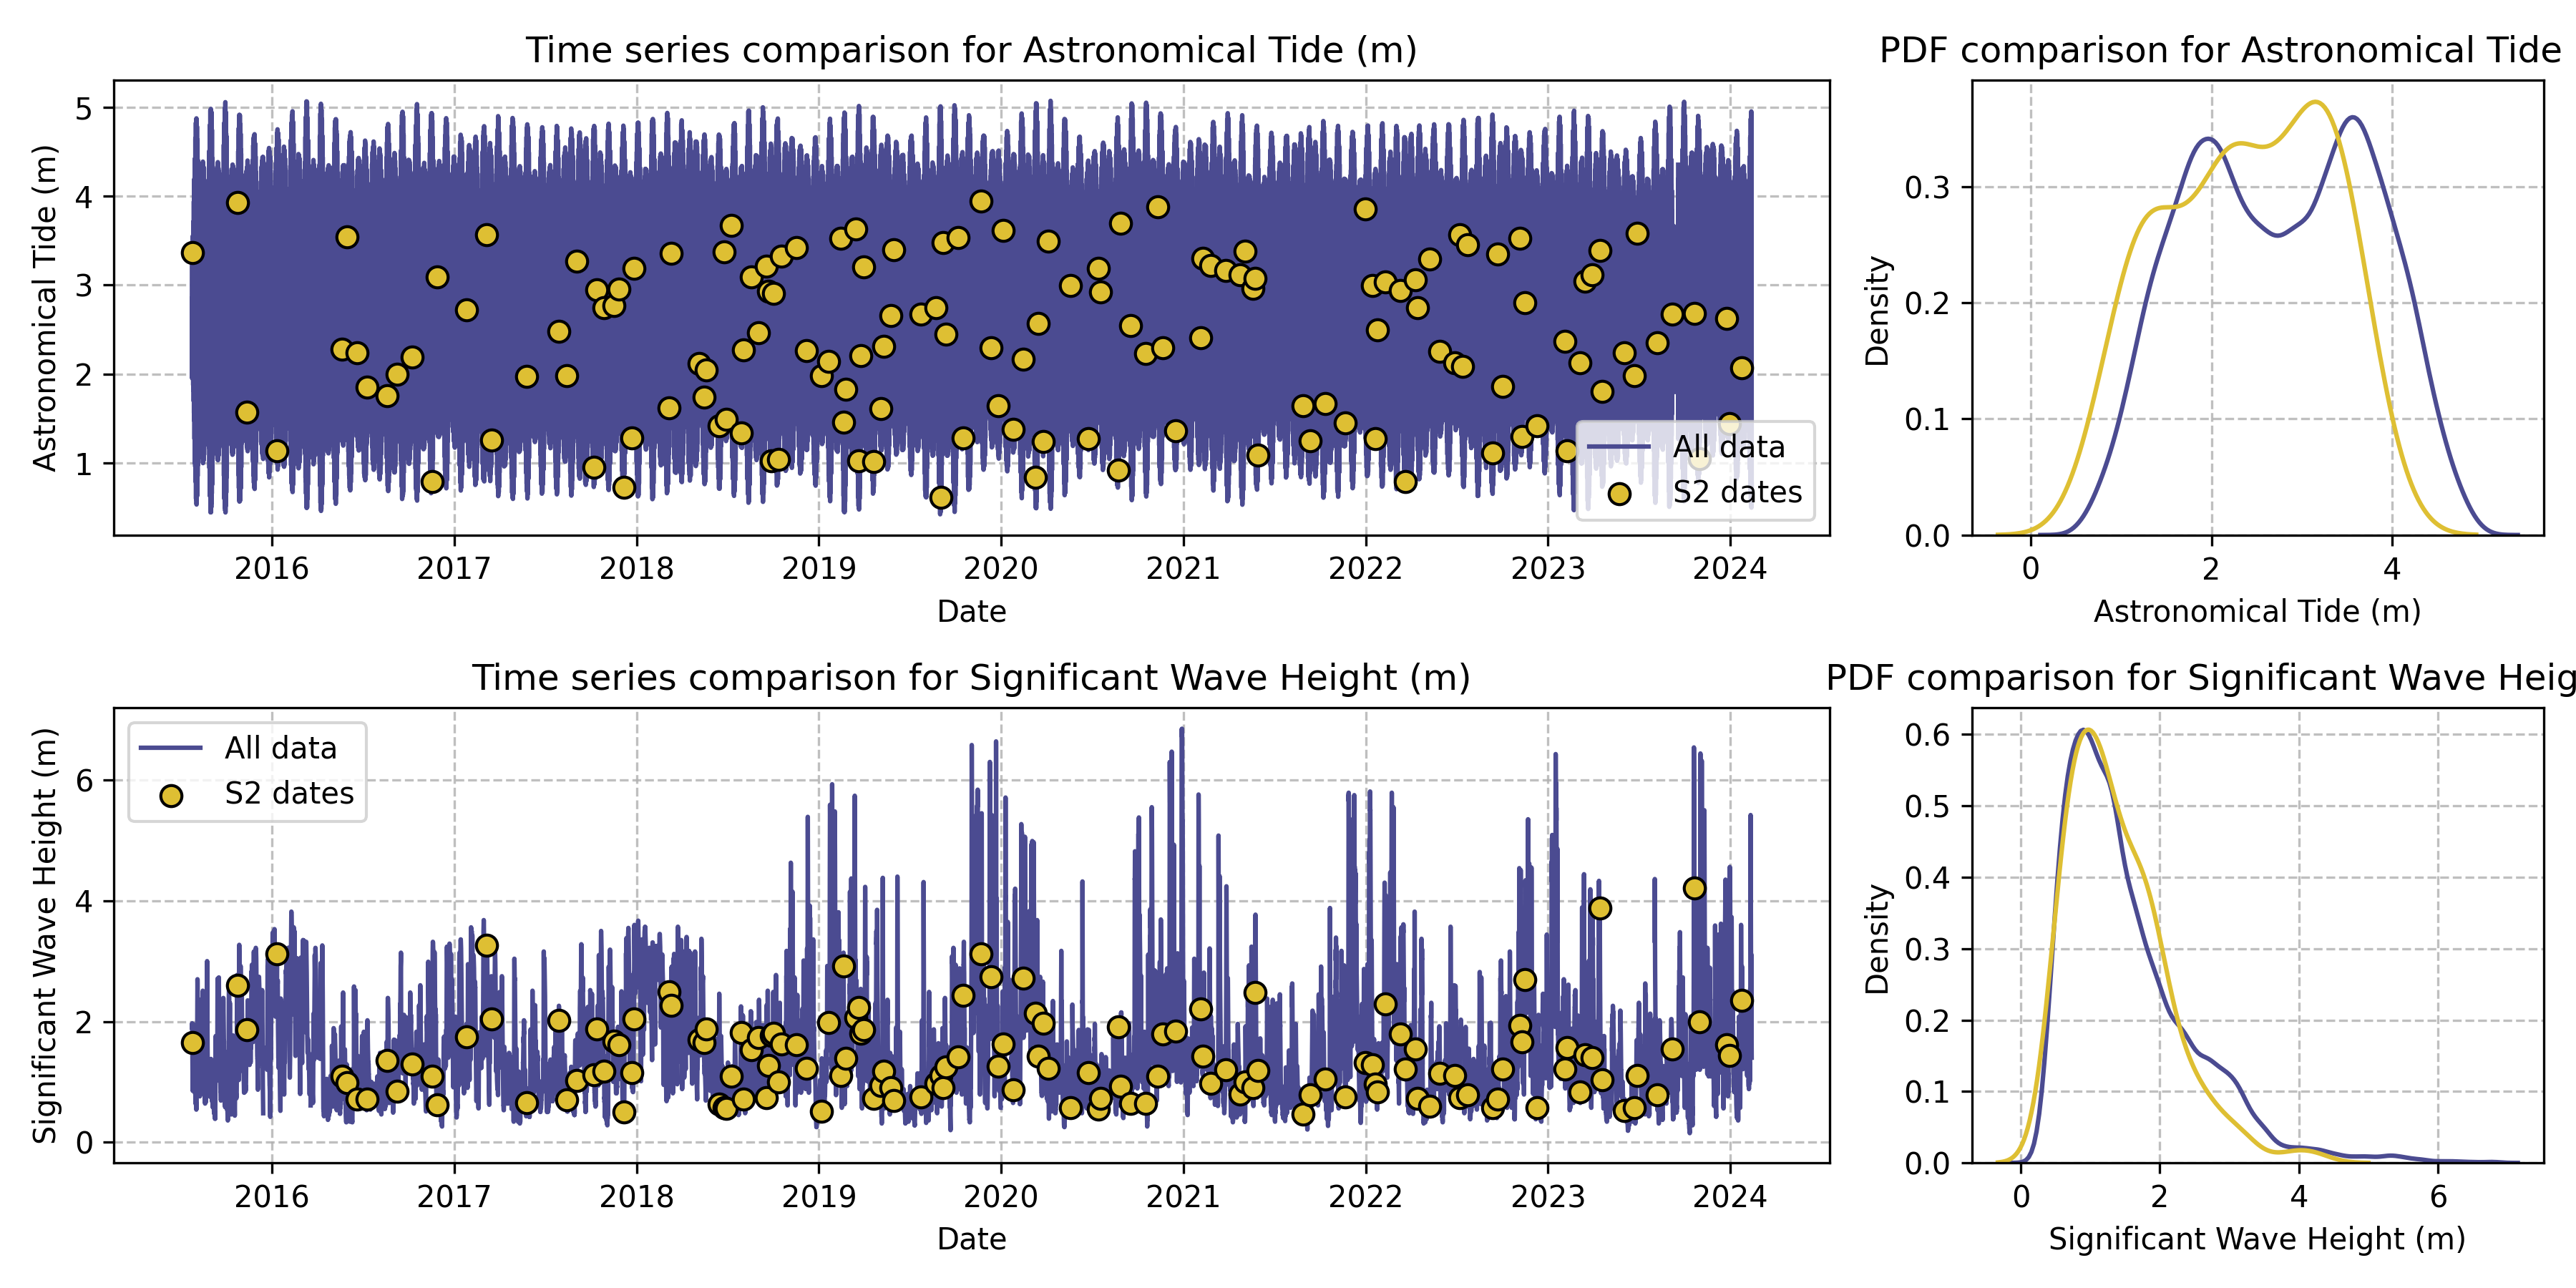
\includegraphics[width=17truecm]{marine_data_comparison.png}
    \caption{Comparison between the continuous oceanographic time-series (purple) and the conditions captured exactly during Sentinel-2 overpasses (yellow dots) for Salinas beach. The top panels highlight the Astronomical Tide, demonstrating the observational bias caused by the sun-synchronous orbit that systematically trims the high-tide peaks. The bottom panels show the Significant Wave Height ($H_s$), which more closely follows the theoretical distribution, albeit missing the extreme storm events.}
    \label{fig:marine_data_comparison}
\end{figure}

\section{Ground Truth Generation (Reference Datasets)}
\label{sec:ground_truth}

To rigorously train the algorithms and benchmark their performance, two distinct sets of Ground Truth (GT) data were generated: pixel-wise multi-class masks for the semantic segmentation models, and continuous vector lines for the final geometric benchmarking evaluation with spectral-index-based methods.

\subsection{Coastal Mask Classes}

To train and validate the Deep Learning models, a highly accurate pixel-level GT dataset was created. Given the complexity of the selected macrotidal environments, a multi-class approach was adopted rather than a simple binary (water/land) classification. The predefined classes were: \textit{water} (undisturbed water bodies), \textit{white-water} (breaking wave foam in the surf zone), \textit{wet sand} (the saturated intertidal zone), and \textit{sand} (dry beach) (see Figure \ref{fig:mask_classes}).

The annotation process was performed manually via photo-interpretation using the DigitalSreeni Image Annotator toolkit \citep{bhattiprolu_digitalsreeni_2026} (Figure \ref{fig:mask_classes}). To ensure the models focus solely on the relevant coastal features, any pixel not manually assigned to one of these four categories was automatically designated as an \textit{ignore\_index}. This ensures that background elements (like urban infrastructure or vegetation) do not interfere with the loss function calculation during training. In total, a dataset comprising 161 image patches (combined from Salinas and El Puntal) was manually annotated and exported into the standardized COCO JSON format.

\begin{figure}[H]
    \centering
    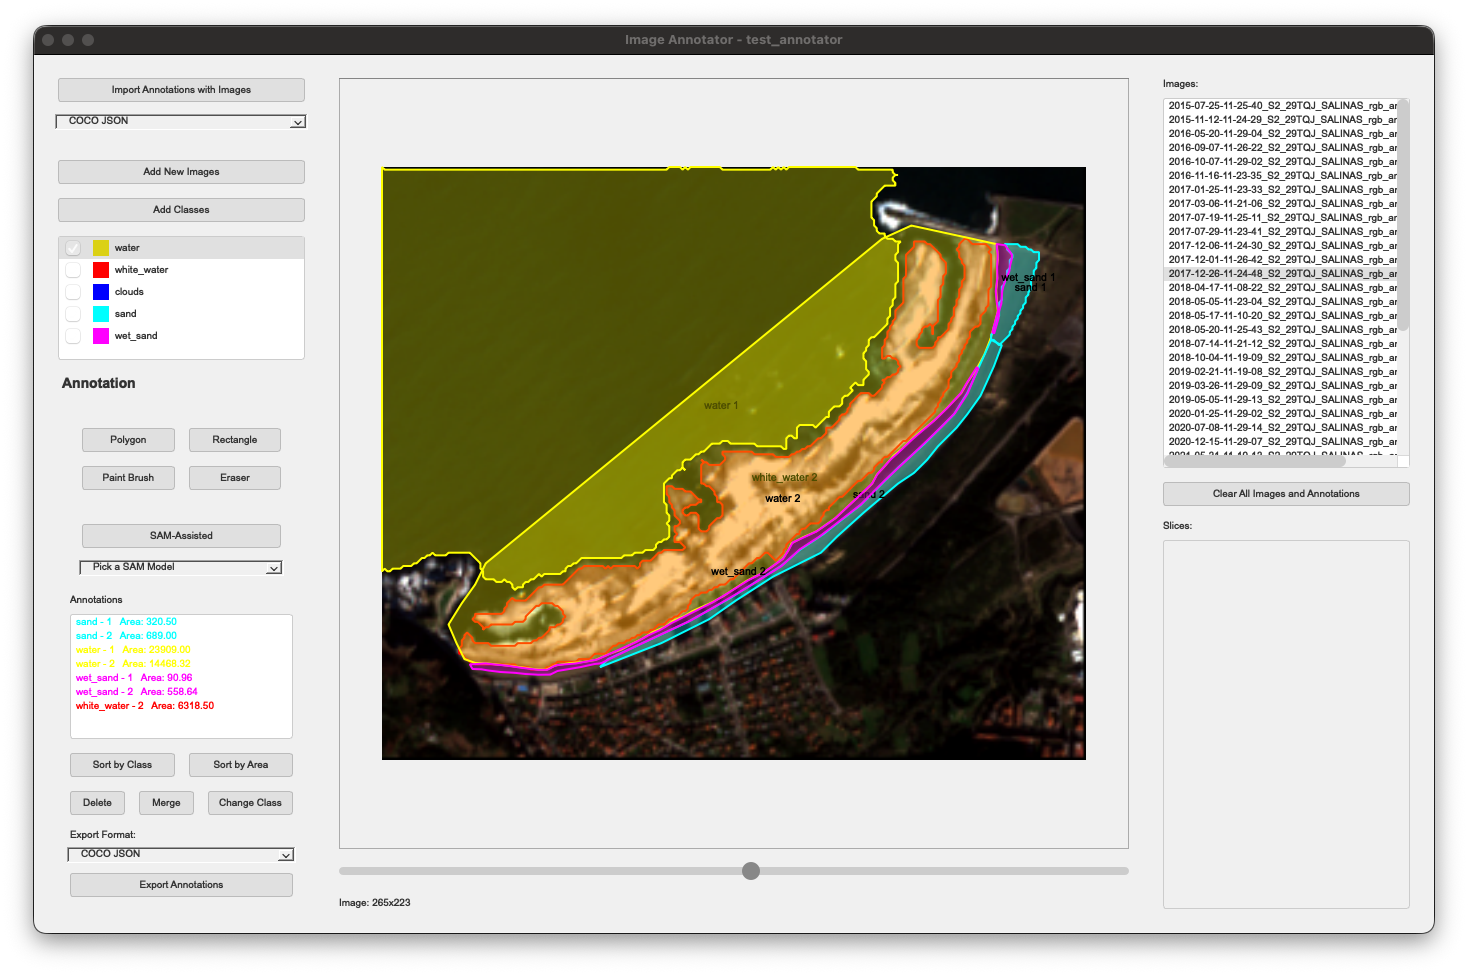
\includegraphics[width=15truecm]{screenshot_example_image_annotator_software.png}
    \caption{Screenshot of the DigitalSreeni Image Annotator software interface (Salinas beach). The overlaid mask displays the four annotated classes: water (yellow), white-water (red), wet sand (purple), and sand (cyan).}
    \label{fig:mask_classes}
\end{figure}

\subsection{Waterline Vectorization}

Alongside the pixel-wise masks, a separate reference dataset consisting of continuous vectorial waterlines was required to evaluate the geometric precision of the shorelines extracted by both the traditional indices and the DL models. For this purpose, a total of 285 reference waterlines (combined from Salinas and El Puntal) were generated.

This process was carried out using the geographic information system software ArcGIS Pro (Figure \ref{fig:vector_waterline}). The instantaneous waterline was manually digitized by tracing the spatial interface between the water mass and the emerged beach. The preprocessed 10~m resolution Sentinel-2 RGB composites were utilized as the visual background reference for this task. The resulting vector lines were then exported as standard Shapefiles (.shp), establishing the absolute geometric Ground Truth for the final benchmarking phase.

\begin{figure}[H]
    \centering
    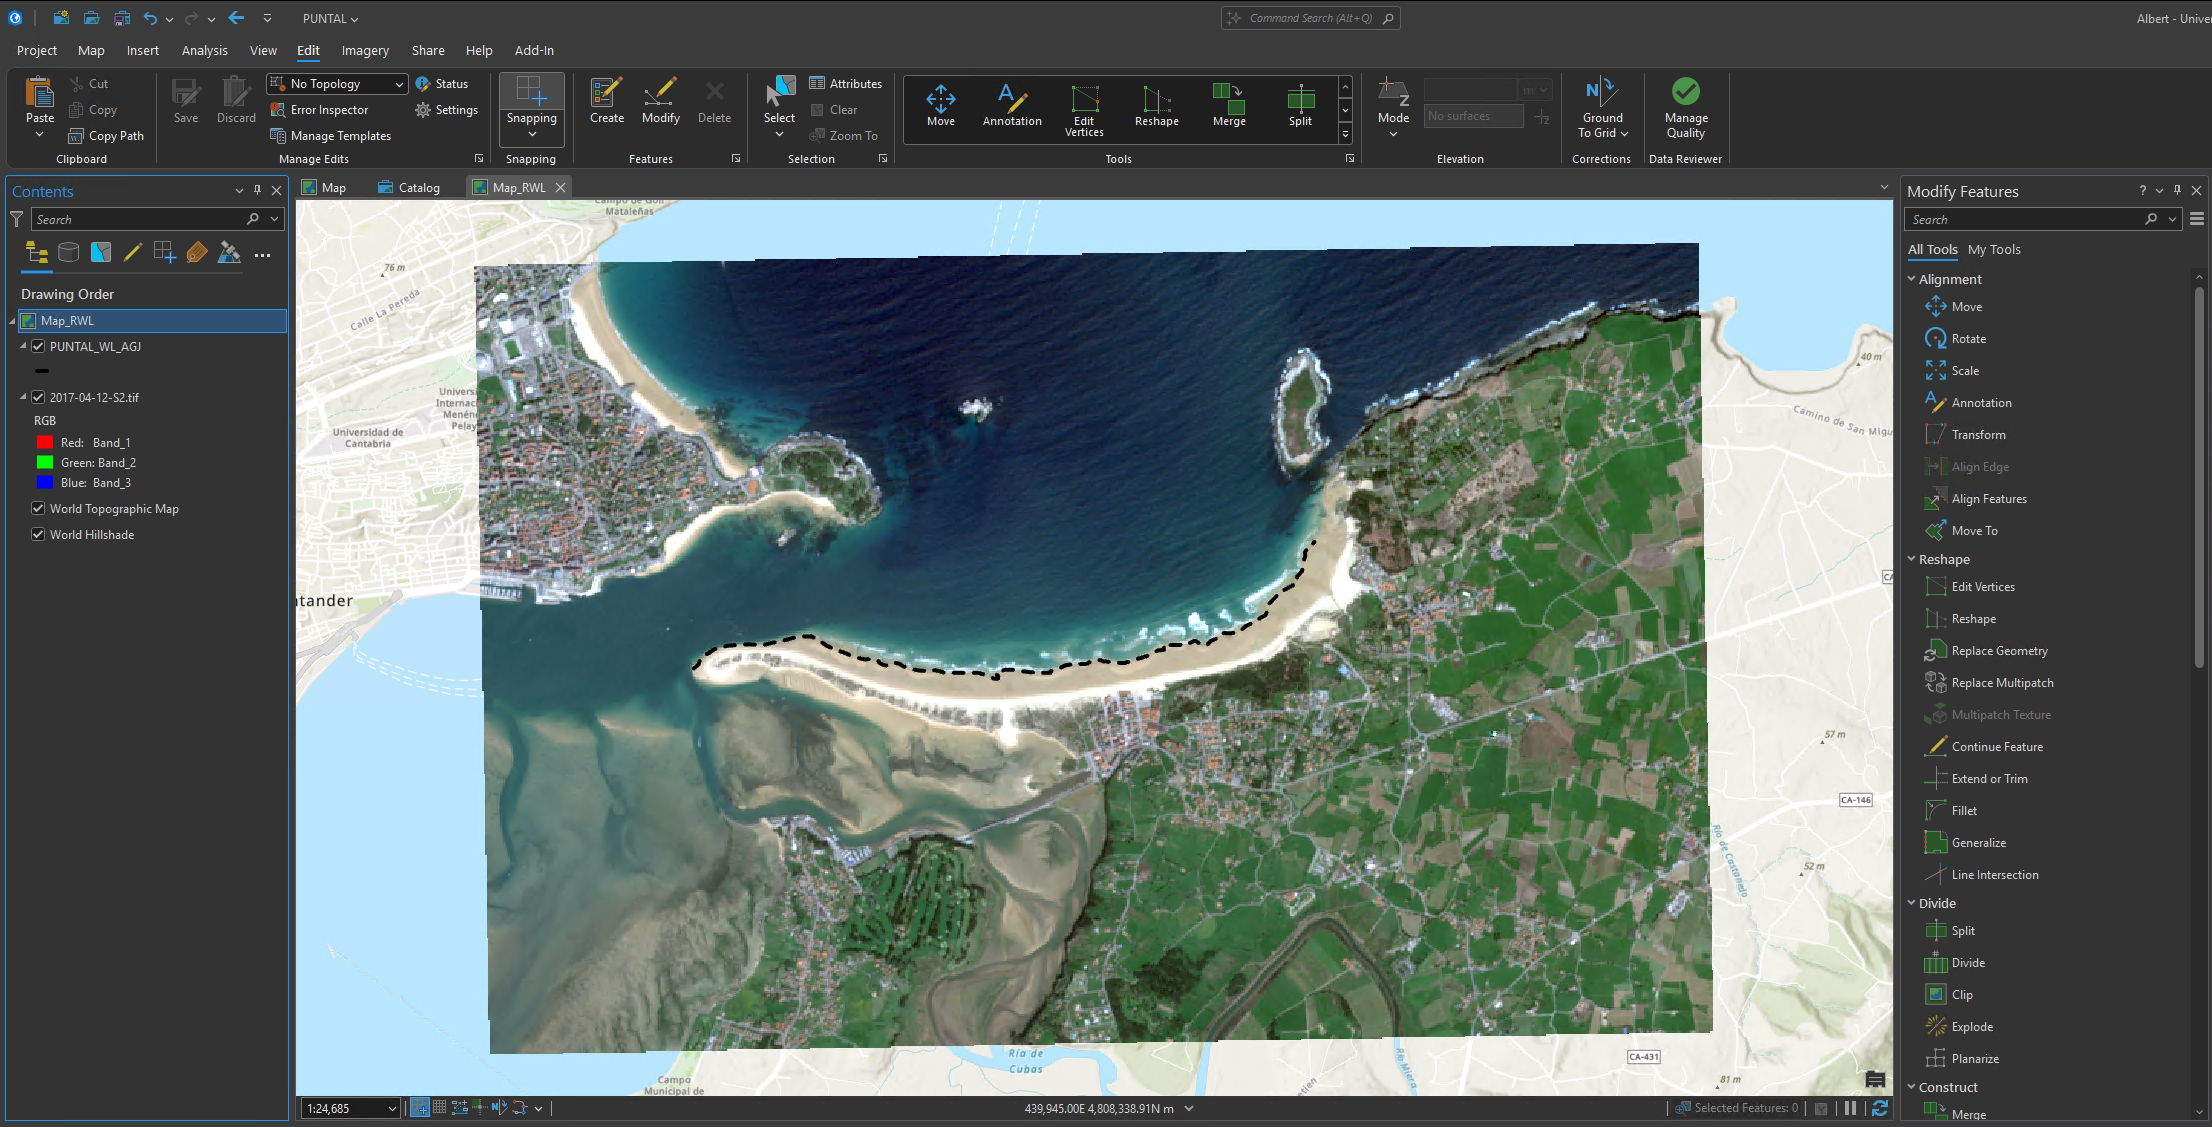
\includegraphics[width=15truecm]{screenshot_vectorization_waterline.png}
    \caption{Screenshot of the ArcGIS Pro interface (El Puntal beach). The manually digitized waterline (black dashed line) is overlaid on the Sentinel-2 RGB composite.}
    \label{fig:vector_waterline}
\end{figure}

\section{Traditional Baseline: Spectral Indices and Thresholding}
\label{sec:baseline_spectral} \label{sec:baseline_spectral}

To establish a solid comparative baseline, we evaluated the performance of four different spectral water indices, coupled with three distinct thresholding techniques. This approach replicates the traditional operational pipelines currently dominating satellite-derived shoreline extraction.

\subsection{Spectral Water Indices}

Spectral indices are mathematical operations applied pixel-by-pixel across the different multispectral bands. By exploiting the distinct reflectance signatures of water and land, they heighten the contrast to facilitate water segmentation. We calculated four indices using the preprocessed Sentinel-2 bands: $\rho_{Blue}$ (B02), $\rho_{Green}$ (B03), $\rho_{NIR}$ (B08), $\rho_{SWIR1}$ (B11), and $\rho_{SWIR2}$ (B12).

\begin{enumerate}
    \item \textbf{Normalized Difference Water Index (NDWI):} Developed by \citet{mcfeeters_use_1996}, it maximizes the typical reflectance of water in the green light while minimizing its low reflectance in the near-infrared (NIR). 
    \begin{equation}
        NDWI = \frac{\rho_{Green} - \rho_{NIR}}{\rho_{Green} + \rho_{NIR}}
    \end{equation}

    \item \textbf{Modified Normalized Difference Water Index (MNDWI):} Proposed by \citet{xu_modification_2006} to address NDWI's difficulty in distinguishing water from built-up land. It replaces the NIR band with the Shortwave-Infrared (SWIR) band, which can penetrate shallow waters and wet environments slightly differently. 
    \begin{equation}
        MNDWI = \frac{\rho_{Green} - \rho_{SWIR1}}{\rho_{Green} + \rho_{SWIR1}}
    \end{equation}

    \item \textbf{Automated Water Extraction Index -- No Shadows (AWEInsh):} Formulated by \citet{feyisa_automated_2014} to maximize the separability of water from dark surfaces or topographic shadows. It combines multiple bands to suppress background noise.
    \begin{equation}
        AWEInsh = 4 \times (\rho_{Green} - \rho_{SWIR1}) - (0.25 \times \rho_{NIR} + 2.75 \times \rho_{SWIR2})
    \end{equation}

    \item \textbf{Subtractive Coastal Water Index (SCoWI):} Recently introduced by \citet{bergsma_shoreliner_2024} specifically for coastal applications with Sentinel-2 data. Unlike normalized ratios, it relies on a subtractive combination designed to better resolve dynamic intertidal zones and suppress the noise from wave breaking foam in macrotidal coasts.
    \begin{equation}
        SCoWI = \rho_{Blue} + 2 \times (\rho_{Green} - \rho_{NIR}) - 0.75 \times \rho_{SWIR1} - 0.5 \times \rho_{SWIR2}
    \end{equation}
\end{enumerate}

\subsection{Thresholding Techniques}

Once the spectral indices are calculated, creating continuous unbouded greyscale intensity maps, a binarization process is required to extract the definitive land-water masks. This is achieved by applying a definitive cutoff threshold. To comprehensively benchmark this step, three different thresholding techniques were evaluated across all indices:

\begin{enumerate}
    \item \textbf{Zero Thresholding:} A static approach fundamentally embedded in the original formulation of normalizated and subtractive water indices. Theoretically, water strongly absorbs NIR/SWIR light, rendering its ratio positive ($>0$), while highly reflective land surfaces yield negative values ($<0$). This method assumes a theoretical zero value as the universal boundary.
    
    \item \textbf{Otsu's Thresholding:} A dynamic, image-adaptive algorithm widely established as the operational standard in modern extraction pipelines. \citet{otsu_threshold_1979} method automatically determines the optimal threshold by calculating the value that minimizes the intra-class variance of the image's histogram under the assumption of a bimodal distribution (distinct water and land classes).

    \item \textbf{Modified Otsu (Local Minimum Histogram):} Because standard Otsu thresholding can be mathematically skewed by disproportionate land/water class distributions or noisy elements unique to macrotidal beaches (like extensive wet sand patches dragging the histogram), we also evaluated a robust refinement proposed by \citet{bergsma_shoreliner_2024}. In this modified approach, once the original Otsu threshold is calculated, the algorithm defines a search interval between the two nearest local maxima on either side of the threshold. The definitive binarization cutoff is then set to the absolute local minimum of the histogram within that specific interval. This adjustment aims to physically anchor the threshold exactly in the valley between the two class distributions, ensuring a more context-aware segmentation.
\end{enumerate}

\section{Deep Learning Semantic Segmentation} \label{sec:dl_models}

To overcome the limitations of threshold-based spectral techniques, the core of this study evaluates the performance of state-of-the-art semantic segmentation neural networks. Similar to the baseline methodology, a systematic grid evaluation was designed by combining different model architectures with various feature-extracting encoders (backbones).

\subsection{Model Architectures}

Three widely recognized semantic segmentation architectures were selected to represent different evolutionary stages and paradigms in computer vision:
\begin{enumerate}
    \item \textbf{U-Net:} A foundational encoder-decoder convolutional architecture originally developed for biomedical imaging \citep{navab_u-net_2015}. Its defining feature is the use of skip connections that concatenate high-resolution feature maps from the encoder directly to the decoder. This enables the precise localization of fine details, which is highly advantageous for delineating a continuous, sharp waterline.
    \item \textbf{DeepLabV3+:} An advanced Convolutional Neural Network (CNN) \citep{chen_encoder-decoder_2018} that utilizes Atrous Spatial Pyramid Pooling (ASPP) to explicitly evaluate the image at multiple scales simultaneously. This architecture allows the model to capture a wider field of view and understand the broader coastal geometry without losing the resolution necessary to trace the complex land-water boundary accurately.
    \item \textbf{SegFormer:} A novel and highly efficient Transformer-based architecture \citep{xie_segformer_2021}. Unlike traditional CNNs, it unifies a hierarchically structured Vision Transformer (ViT) encoder (which avoids strict positional encoding interpolation issues) with a lightweight multilayer perceptron (MLP) decoder. It excels at incorporating global contextual information, which is critical for navigating the semantic ambiguity of extensive wave splash and dark wet sand.
\end{enumerate}

\subsection{Encoders}

The feature extraction capability of a segmentation network relies heavily on its encoder backbone. To balance computational efficiency and feature extraction depth, two distinct encoder families were chosen:
\begin{itemize}
    \item \textbf{EfficientNet:} Representing the Convolutional Neural Network paradigm, we selected the \textit{efficientnet-b4} (lighter, 17M params) and \textit{efficientnet-b7} (heavier, 63M params) \citep{tan_efficientnet_2019}. EfficientNet models are designed to optimize the trade-off between network depth, width, and resolution, making them robust for various image recognition tasks while maintaining computational efficiency.
    \item \textbf{Mix Transformer (MiT):} Representing the hierarchical Vision Transformer paradigm, we selected the \textit{mit\_b2} (lighter, 24M params) and \textit{mit\_b4} (heavier, 60M params) variants \citep{xie_segformer_2021}. These transformers are naturally designed to extract both local and global attention features.
\end{itemize}

It is worth noting a deliberate methodological divergence in this study's experimental matrix. From a strict theoretical standpoint, CNN-based decoders (such as U-Net or DeepLabV3+) are traditionally paired with CNN-based encoders, whereas Transformer decoders (like SegFormer) are paired with ViT encoders to maintain architectural purity. However, preliminary empirical testing during this project revealed an interesting dynamic: hybridizing the architectures (specifically, injecting the global-context awareness of the MiT transformer encoders into the precise local-feature CNN decoders) yielded remarkably superior and robust segmentation results in the most challenging coastal scenes. Consequently, to fully explore this advantage, an exhaustive grid approach was adopted where all candidate encoders (EfficientNet-B4, EfficientNet-B7, MiT-B2 and MiT-B4) were systematically crossed and tested across all three model architectures.

\subsection{Training Setup}
\label{sec:training_setup}

To ensure a fair and equitable comparison, all deep learning models were fine-tuned following an identical hyperparameter configuration and optimization strategy. 

Prior to training, the annotated dataset was partitioned into a strict 80\% training and 20\% testing split, with a subset of the training data allocated for internal epoch validation. To prevent the models from overfitting to a specific tidal state or geographical morphology, this subdivision was strictly stratified based on both the associated instantaneous tide values (acquired during the preprocessing stage) and the specific study area (Salinas or El Puntal). This rigorous stratification ensures that images capturing high-tide and low-tide scenarios, as well as sheltered and exposed conditions, were equitably distributed. Consequently, the networks were trained and evaluated on a perfectly balanced representation of the highly dynamic intertidal zones.

The models were trained for a maximum of 100 epochs using a batch size of 16 patches. To minimize the loss function while mitigating overfitting, the AdamW optimizer (Adam with weight decay) was employed with an initial learning rate of $5 \times 10^{-4}$ and a weight decay coefficient of $1 \times 10^{-4}$. Furthermore, a dynamic learning rate scheduler (\textit{ReduceLROnPlateau}) was implemented, which reduces the learning rate by a factor of 0.5 if the validation loss plateaus for 5 consecutive epochs. Early stopping was also configured with a patience of 15 epochs to stop training when no further validation improvements were observed, thereby preventing over-parameterization and saving computational resources.

Given the multi-class formulation of the dataset, the standard Cross-Entropy Loss function was utilized. Crucially, the loss calculation explicitly ignored any pixel labeled as \textit{ignore\_index} (value 255) during the Ground Truth generation phase, forcing the networks to focus exclusively on learning the target coastal features (water, white-water, wet sand, and sand) without penalization from urban or vegetated background areas.

Finally, to significantly increase the model's robustness and generalization capabilities against varying beach orientations and viewing angles, a spatial data augmentation pipeline was strictly applied to the training set. Utilizing the Albumentations library, image patches were randomly subjected to horizontal flips, vertical flips, 90-degree rotations, and transpositions, each with a 50\% probability during every training epoch. In contrast, the validation and test datasets were evaluated using the original, unaugmented distribution of the image patches.

To guarantee the statistical reliability of the results and account for the stochastic nature of network initialization and optimization, the training process for each model configuration (architecture-encoder pair) was repeated 10 independent times under varying random seeds. Following each set of iterations, the optimal run was selected based on its segmentation performance strictly along the coastal boundary zone. This was achieved by collapsing the multi-class predictions into binary masks (water versus non-water) and computing the Intersection over Union (IoU) exclusively within a reduced buffer region adjacent to the ground-truth waterline. A comprehensive explanation of this boundary-focused pixel-based evaluation and class mapping strategy is provided later in Section \ref{sec:pixel_eval}.

\subsection{Hardware and Software Specifications}
\label{sec:hardware_software}

All computational routines throughout this project, including data preprocessing, vector operations, and statistical evaluation, were developed in Python. The functional source code containing the reproducible experimental pipelines has been open-sourced and published in a public GitHub repository \citep{github_sentinel2-coastline-benchmarking}.

For the deep learning implementation, the \textit{segmentation\_models.pytorch} library was utilized as the primary API, providing structured and accessible implementations of the U-Net, DeepLabV3+, and SegFormer architectures. Rather than initializing the feature extraction encoders with random values, they were instantiated utilizing pre-trained weights from the \textit{ImageNet} dataset (\texttt{encoder\_weights="imagenet"}). This transfer learning strategy accelerates network convergence and provides the models with a pre-existing, robust understanding of fundamental geometric features such as edges and textures before fine-tuning them on the coastal domain.

Regarding hardware utilization, the computationally intensive task of training the semantic segmentation networks across all configurations, encoders, and random seeds was executed on a dedicated desktop PC equipped with an NVIDIA RTX 3060 GPU. Conversely, all other tasks (including dataset preprocessing, downloading of oceanographic data, programmatic thresholding of spectral indices, model inference, and the comprehensive spatial and geometric evaluations) were executed on an Apple MacBook Air featuring an M5 Apple Silicon chip.

\section{Waterline Extraction Pipeline}
\label{sec:waterline_pipeline}

To systematically compare the performance of traditional spectral indices against the Semantic Segmentation Deep Learning models, it is necessary to translate their respective pixel-based outputs into continuous, comparable geographic vectors. This process, known as sub-pixel contouring, is critical for achieving the high spatial precision required for shoreline monitoring.

For the traditional baselines (see Section \ref{sec:baseline_spectral}), the extraction pipeline follows a strict three-step sequence. First, continuous intensity rasters are computed using the mathematical formulations of the four selected spectral water indices (e.g., MNDWI, SCoWI). Second, discrete binary masks ("water" versus "non-water") are created by applying the cutoff threshold values evaluated for each method (Zero, Otsu, and Modified Otsu). Third, the final waterlines are generated in vector format by utilizing the Marching Squares contouring algorithm \citep{lorensen_marching_1987} to trace a smooth boundary where the binary mask transitions from 0 to 1. This algorithm effectively interpolates the exact sub-pixel location of the water boundary, allowing for a more precise vector representation of the waterline.

Conversely, for the Deep Learning models, the segmentation output requires a slight mathematical adaptation to maximize its utility for vectorization. After processing a $128 \times 128$ image patch, the neural network outputs multi-class prediction logits. These logits are converted into confidence scores (ranging from 0.0 to 1.0) using a Softmax activation function. Subsequently, the pixels segmented as \textit{water} and \textit{white-water} classes are collapsed into a single "water" class, while the \textit{wet sand} and \textit{sand} classes are collapsed into a single "non-water" class. Then, the final waterlines are extracted using the same Marching Squares contouring algorithm as in the traditional pipeline, applied to the resulting binary mask. This ensures that the final output from both approaches is directly comparable in terms of format and spatial precision.

Finally, for both traditional and DL approaches, the individual continuous line segments extracted in each image are merged together. A morphological length filter is then applied, discarding any discontinuous segments shorter than a minimum threshold length. This filtering effectively removes small landlocked ponds, temporary tidal puddles, and isolated false positive artifacts, resulting in a single, robust, and continuous vector representation of the waterline.

\section{Evaluation Methodology}
\label{sec:evaluation_methodology}

To comprehensively assess the performance of the tested methodologies, the accuracy of the outputs was evaluated across two distinct structural domains: a purely pixel-based evaluation of the semantic segmentation masks, and a rigorous geometric validation of the final continuous vector waterlines. In addition to these core evaluations, an independent empirical analysis of the sand reflectance and colorimetry was conducted to physically contextualize the spectral challenges inherent to the study sites, particularly in Salinas. This analysis is crucial to understand the underlying physical factors that may influence the performance of both traditional and AI-based extraction methods.

\subsection{Sand Reflectance and Colorimetric Assessment}
\label{sec:sand_reflectance}

Prior to the core pixel-based and geometric evaluations, an independent empirical analysis was conducted to quantify the spectral differences of the supratidal sand between the two study sites. This assessment was designed to test the hypothesis that the severe degradation in the segmentation performance of traditional spectral indices at Salinas is fundamentally driven by the physical coloration of its beach. Specifically, the accumulation of dark carbonaceous shales and coal creates a low-reflectance environment that critically mimics the spectral signature of water, in stark contrast to the highly reflective, golden-colored sand of El Puntal.

To quantitatively verify this spatial divergence without manual intervention across the entire temporal dataset, a strict constraint-based methodology was implemented to isolate the spectral signature of dry sand. First, a single "candidate image" was carefully selected for each beach. These reference images were chosen based on optimal conditions for dry beach exposure: cloud-free weather, minimum astronomical tide, and low energetic wave conditions. Utilizing these candidate scenes, a static Region of Interest (ROI) polygon was manually digitized strictly over the emerged, dry sand area of each beach.

To extract a reliable time-series of sand reflectance values, it was imperative to ensure that the static ROIs were not contaminated by water or wave run-up in subsequent images. Therefore, the complete dataset was temporally filtered using the historical oceanographic metadata. For each beach, only the satellite acquisitions where the instantaneous tidal level, significant wave height ($H_s$), and peak period ($T_p$) were equal to or strictly lower than those of their respective candidate image were retained. This rigorous hydrodynamic thresholding guarantees that the pixels contained within the static ROIs predominantly represent undisturbed dry sand throughout the evaluated subset.

Finally, using the preprocessed Sentinel-2 Level-2A imagery, two specific physical metrics were calculated for all pixels within the isolated ROIs to characterize the brightness and colorimetry of the sand:

\begin{enumerate}
    \item \textbf{Mean Visible Reflectance ($\bar{\rho}_{RGB}$):} Calculated as the unweighted arithmetic mean of the Red, Green, and Blue bands. This metric serves as a direct proxy for the overall albedo of the sand in the visible spectrum, evaluating its absolute darkness.
    \begin{equation}
        \bar{\rho}_{RGB} = \frac{\rho_{Red} + \rho_{Green} + \rho_{Blue}}{3}
    \end{equation}

    \item \textbf{Red-Blue Differential ($\Delta_{R-B}$):} This metric evaluates the colorimetric slope of the target. Standard golden sand typically exhibits strong reflectance in the red spectrum and higher absorption in the blue, yielding a large positive differential. Conversely, carbonaceous dark sand presents a flatter, wavelength-independent spectral response (grey/black), resulting in a significantly lower differential.
    \begin{equation}
        \Delta_{R-B} = \rho_{Red} - \rho_{Blue}
    \end{equation}
\end{enumerate}

By comparing the probabilistic distributions of these two metrics between Salinas and El Puntal, this analysis establishes a measurable geologic and spectral baseline. This baseline is crucial to physically contextualize the statistical geometric errors evaluated in the subsequent algorithmic sections.

\subsection{Pixel-based Evaluation}
\label{sec:pixel_eval}

Evaluating segmentation performance across full coastal scenes introduces a significant statistical bias due to extreme spatial class imbalance. When traditional pixel-based metrics are calculated over the entire image grid, their scores are highly susceptible to artificial inflation. Because the vast majority of pixels in a standard satellite patch belong to unambiguous, easily classified regions (such as the open ocean or stable inland areas) a model can achieve exceptionally high scores even if it completely misidentifies the delicate land-water boundary. Since the actual intertidal transition zone constitutes only a minuscule fraction of the total image, critical segmentation errors along the shoreline are mathematically overshadowed by the large number of correctly classified background pixels.

To counteract this statistical bias, a highly constrained, boundary-focused evaluation protocol was designed. Initially, the native multi-class structure of the ground-truth masks (and the corresponding Deep Learning predictions) was mathematically collapsed into binary domains: \textit{water} and \textit{white-water} were unified under the definitive "Water" class, while \textit{wet sand} and \textit{sand} were clustered into "Land". Any unannotated background elements assigned with the \textit{ignore\_index} (value 255) were strictly excluded from the calculations.

Subsequently, a symmetric spatial buffer equivalent to 10 pixels (representing a physical distance of 100 meters, given Sentinel-2's native 10 m resolution) was dynamically generated exclusively around the exact ground-truth waterline (see Figure \ref{fig:evaluation_mask}). The evaluation was strictly constrained to this 100-meter buffer zone algorithmically identified using the Euclidean Distance Transform. By completely masking out the deep water body and the inland sectors, the models were forced to perform, and be penalized, exclusively on the challenging semantic ambiguity of the intertidal zone.

\begin{figure}[H]
    \centering
    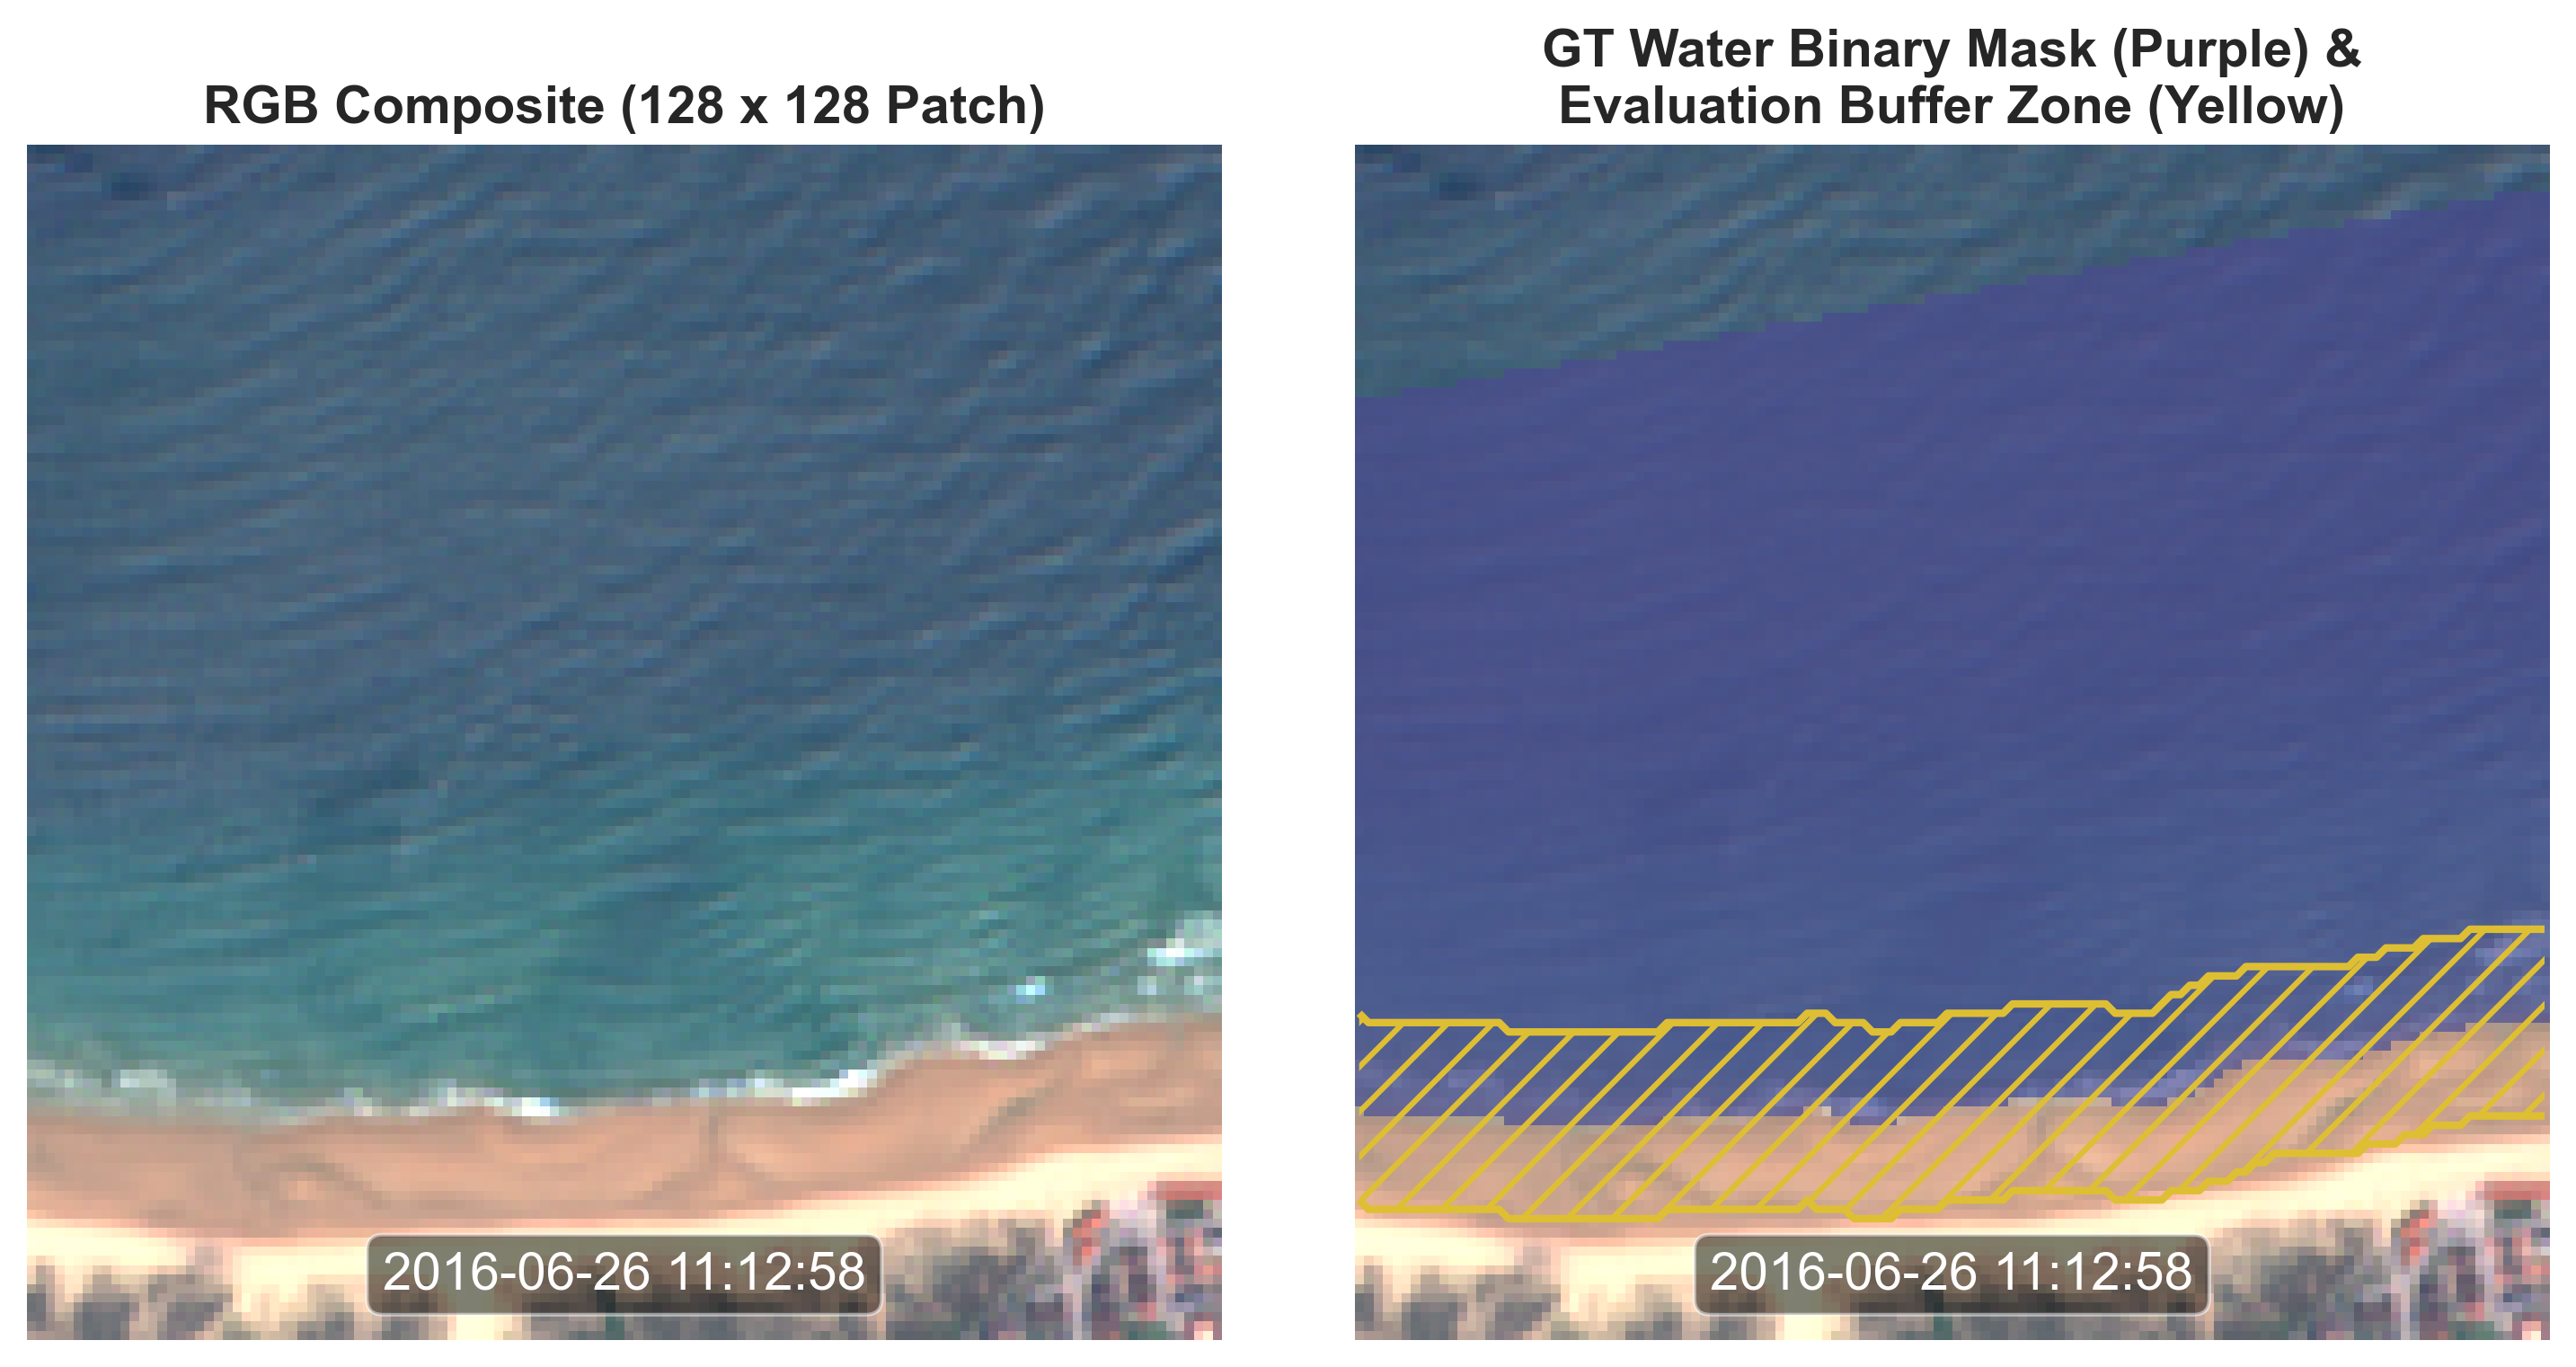
\includegraphics[width=15truecm]{boundary_zone_visualization.png}
    \caption{Example of the pixel-based evaluation mask. The left panel shows the original RGB image. The dynamic evaluation buffer (right) highlights the 10-pixel zone around the GT waterline where the pixel-based metrics are calculated, effectively excluding the deep water and inland areas from the evaluation.}
    \label{fig:evaluation_mask}
\end{figure}

Within this restricted boundary zone, the segmentation performance was quantified using two standard computer vision metrics:
\begin{itemize}
    \item \textbf{Intersection over Union (IoU):} Also known as the Jaccard Index, it calculates the ratio of the intersection of the predicted and ground-truth water masks to their union. It is a strict metric that heavily penalizes false positives (e.g., misclassifying wet sand as water).
    \item \textbf{Dice Coefficient:} Similar to the IoU but assigning double weight to the correct positive predictions, providing a slightly more forgiving, harmonized measure of the overlap.
\end{itemize}

\subsection{Geometric Evaluation}

While the pixel-based evaluation determines how well a model categorizes the image grid, the geometric evaluation translates those results into the real-world metric required by coastal engineers: tracking the physical position of the coast in meters. 

To achieve this, the continuous vectorial waterlines derived from both the traditional sub-pixel contouring and the Deep Learning probability maps (as described in Section 3.6) were benchmarked against the manually digitized Ground Truth shapefiles. This assessment was performed using the standard shore-perpendicular cross-shore transect methodology (Figure \ref{fig:transect_methodology}).

First, a fixed, static landward baseline roughly parallel to the general orientation of the beach is established. From this baseline, perpendicular transects were cast seaward at evenly spaced intervals (i.e., every 50 meters) along the entire longitude of the study area. For each individual transect ($i$), the intersection points with both the predicted vector waterline and the reference GT waterline were mathematically calculated. The 1D Euclidean distance from the baseline to these two points constitutes the basis for the extraction error at that specific profile. It's worth mentioning that, within the specific context of remote sensing applied to waterline monitoring, this calculated error (the spatial distance between the actual and the predicted position) is widely referred to in the literature as the extraction "offset". Mathematically, the offset for a specific transect $i$ is formulated as:

\begin{equation}
    Offset_i = |d_{mod,i} - d_{obs,i}|
\end{equation}

where $d_{mod,i}$ represents the cross-shore distance from the baseline to the \textit{modeled} (predicted) shoreline derived from either the DL or index-based methods at transect $i$, and $d_{obs,i}$ represents the distance to the \textit{observed} reference shoreline extracted from the Ground Truth.

\begin{figure}[H]
    \centering
    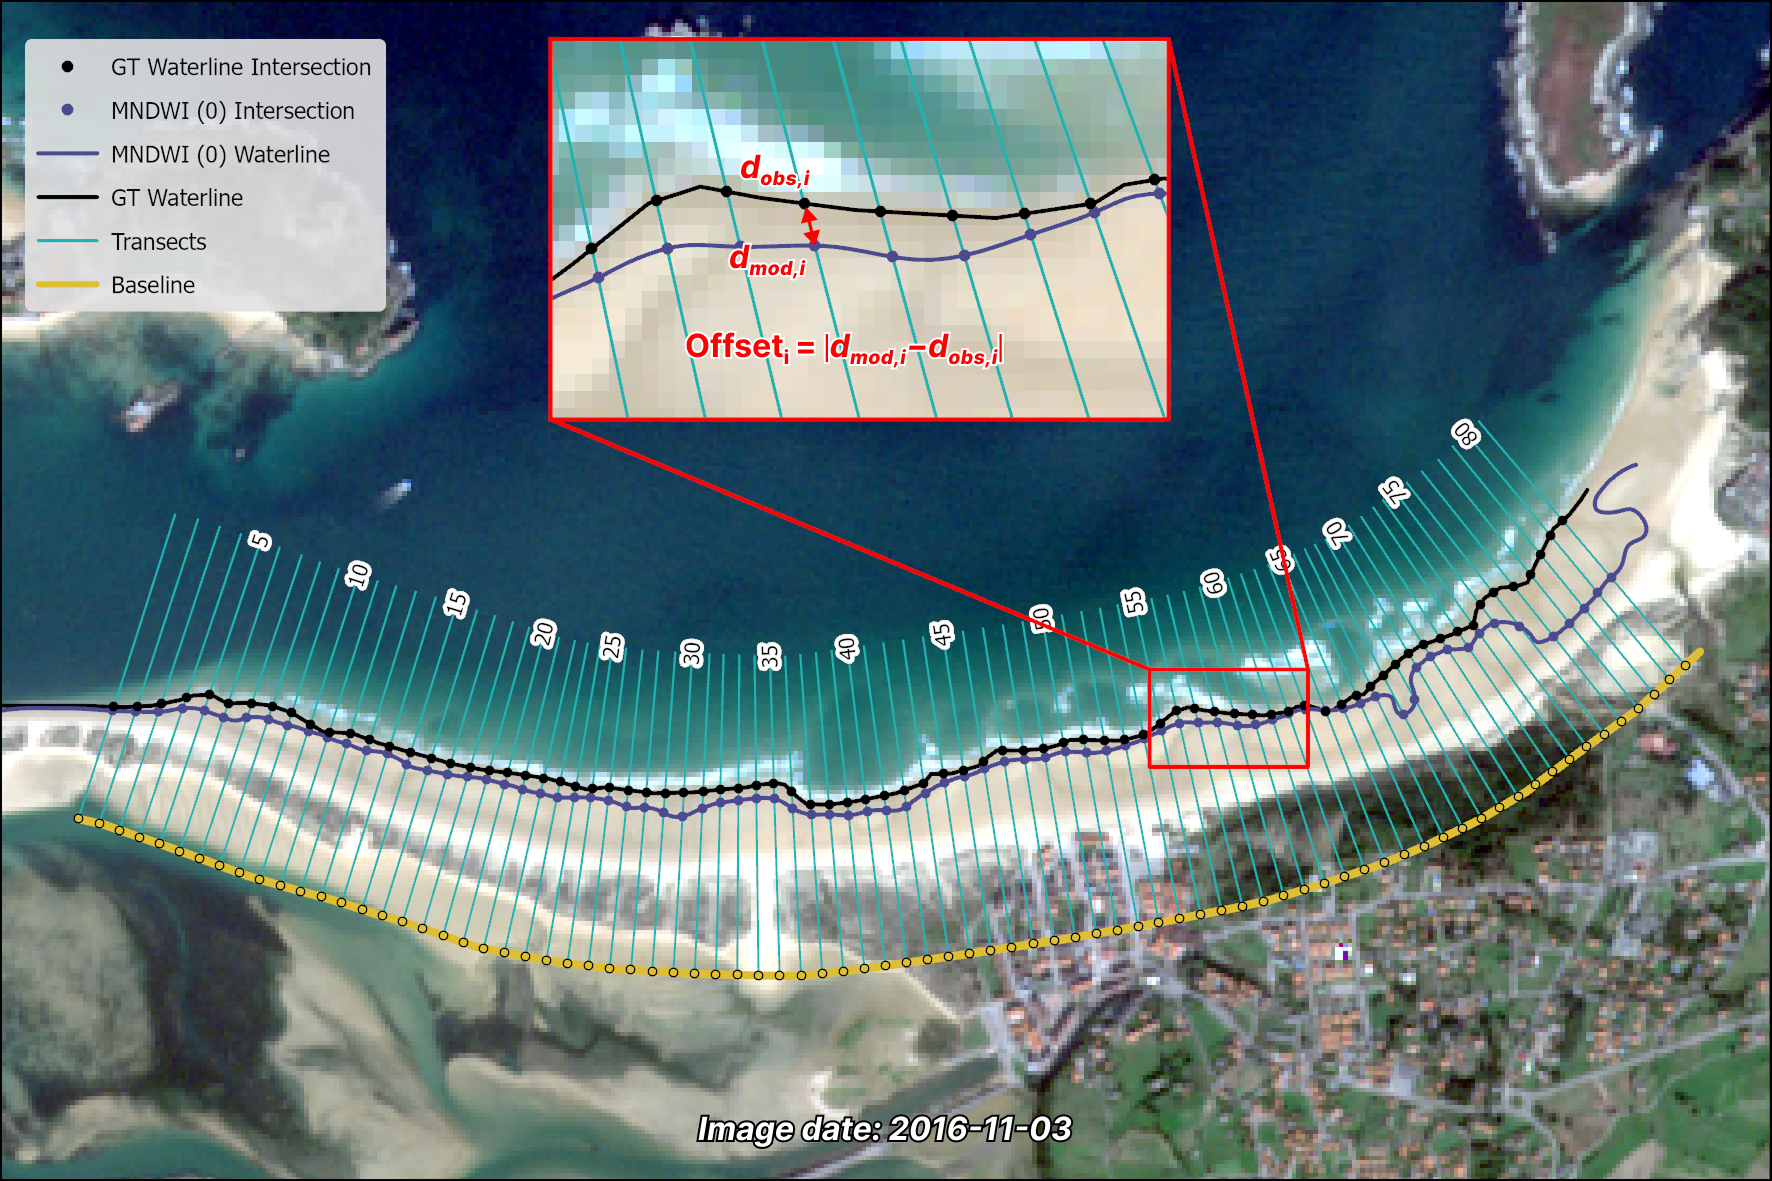
\includegraphics[width=15truecm]{figure_example_offset_calc.png}
    \caption{Example of the perpendicular transect methodology for geometric evaluation. The black line represents the manually digitized GT waterline, while the purple line represents the predicted waterline from either the DL or index-based method (in this case, MNDWI using Zero threshold). The yellow line is the fixed landward baseline. The cyan lines are the perpendicular transects cast from the baseline to the predicted and GT waterlines. The offset is calculated as the absolute distance between the intersection points of the predicted and GT waterlines along each transect.}
    \label{fig:transect_methodology}
    
\end{figure}

By aggregating the distances recorded across all intersecting transects for a given satellite image, four robust statistical metrics were computed:
\begin{itemize}
    \item \textbf{Median Absolute Deviation/Error (MAD):} The median of the absolute offsets. Because it relies on the median rather than the mean, MAD is highly robust against severe outliers (such as specific transects with an extreme errors due to a contouring artifact or specific complex scenarios because a highly energetic wave event), offering a highly representative value of the "typical" coastline error.
    \item \textbf{Interquartile Range (IQR):} The range between the 25th and 75th percentiles of the offsets. This metric provides insight into the variability and consistency of the extraction errors across the entire coastline.
    \item \textbf{Mean Absolute Error (MAE):} The average of the absolute values of the offsets. Unlike Bias, MAE does not allow positive and negative errors to cancel each other out, providing a straightforward measure of the average magnitude of the extraction error.
    \item \textbf{Mean Error (Bias):} The arithmetic average of all transect distances. It evaluates the systematic tendency of the model to underestimate or overestimate the water extent. A negative Bias indicates a systematic landward offset (the model predicts water further inland than reality, a common failure over wet sand), while a positive Bias indicates a seaward bias.
    \item \textbf{Root Mean Square Error (RMSE):} Measures the overall magnitude of the spatial discrepancy. Because it squares the errors before averaging, the RMSE strongly penalizes extreme localized deviations (such as the model mistakenly tracing an isolated intertidal pool or wave foam), providing a conservative and reliable metric of the extraction's operational viability.
    \item \textbf{Coefficient of Determination ($R^2$):} Evaluates the degree of correlation between the predicted and observed shoreline positions across all transects. An $R^2$ value close to 1 indicates a strong linear relationship, while a value close to 0 suggests no correlation.
\end{itemize}

\textbf{Statistical Analysis Framework:}

Once the aforementioned cross-shore metrics were derived for the entire dataset, a comprehensive statistical framework was established to interpret the results and facilitate a structured comparison in Chapter 4. This framework relies on several analytical approaches to evaluate the models across different dimensions:

\begin{itemize}
    \item \textbf{Global and Distributional Analysis:} To compare the overarching performance between Index-based and Deep Learning families, as well as to identify morphological dependencies, the aggregated offset distributions are analyzed using boxplots and violin plots segregated by study area.
    \item \textbf{Spatial Bias Evaluation:} Beyond absolute error magnitudes (MAE), the systematic orientation of the errors is evaluated. Hexbin scatter plots are utilized to map the extraction bias (landward vs. seaward) across the cross-shore distances, revealing intrinsic behaviors of specific architectures and thresholding techniques.
    \item \textbf{Environmental Dependency Assessment:} To isolate the sources of error variability, the extraction offsets are cross-referenced with hydrodynamic forcing. Specifically, the offsets are analyzed across categorical quartiles of tidal levels and significant wave heights ($H_s$) to assess model degradation under complex coastal dynamics.
    \item \textbf{Cross-Site Generalization:} The robustness of the models is quantified by calculating the MAE difference ($\Delta$ MAE) between the sheltered baseline site (El Puntal) and the highly dynamic stress-test site (Salinas). A minimized $\Delta$ MAE serves as the primary indicator of a model's capacity to generalize without overfitting to local morphologies.
    \item \textbf{Multi-Criteria Ranking:} Finally, all computed metrics (RMSE, MAE, MAD, Bias, and $R^2$) are synthesized and normalized into heatmaps and bump charts to produce a definitive, objective ranking of the top-performing global configurations.
\end{itemize}

\subsection{Summary of Evaluated Models}

To provide a clear overview of the entire experimental matrix, Table \ref{tab:evaluation_recap} summarizes all the models and configurations tested in this project, explicitly detailing which evaluation protocols were applied to each.

\begin{table}[H]
    \centering
    \caption{Summary of the evaluated extraction methods, their configurations, and the corresponding applied evaluation protocols.}
    \vspace{0.1cm}
    \renewcommand{\arraystretch}{1.4}
    \resizebox{\textwidth}{!}{
    \begin{tabular}{l l l c c}
        \hline
        \textbf{Category} & \textbf{Base Model / Index} & \textbf{Evaluated Variations / Encoders} & \textbf{Pixel-based Eval.} & \textbf{Geometric Eval.} \\
        \hline
        \multirow{4}{*}{Spectral-based} 
        & NDWI & Zero, Otsu, Modified Otsu & No & Yes \\
        & MNDWI & Zero, Otsu, Modified Otsu & No & Yes \\
        & AWEInsh & Zero, Otsu, Modified Otsu & No & Yes \\
        & SCoWI & Zero, Otsu, Modified Otsu & No & Yes \\
        \hline
        \multirow{3}{*}{Deep Learning-based} 
        & U-Net & EfficientNet-B4/B7, MiT-B2/B4 & Yes & Yes \\
        & DeepLabV3+ & EfficientNet-B4/B7, MiT-B2/B4 & Yes & Yes \\
        & SegFormer & EfficientNet-B4/B7, MiT-B2/B4 & Yes & Yes \\
        \hline
    \end{tabular}
    }
    \label{tab:evaluation_recap}
\end{table}


\chapter{Results}

\section{Physical Context: Sand Reflectance and Colorimetric Assessment}
\label{sec:results_sand_reflectance}

To establish the physical baseline of the study areas and test the hypothesis regarding the spectral ambiguity at Salinas beach, the brightness and colorimetry of the supratidal sand were quantified. Following the strict hydrodynamic filtering detailed in Section \ref{sec:sand_reflectance}, a total of 28 optimal scenes for El Puntal and 24 scenes for Salinas were retained for this analysis. Figure \ref{fig:reflectance_boxplots} illustrates the probabilistic distributions of the two evaluated metrics across both locations.

The Mean Visible Reflectance ($\bar{\rho}_{RGB}$) demonstrates a significant disparity in the overall albedo between the two sites. El Puntal exhibits highly reflective sand with a mean intensity value of $2313.09 \pm 312.91$. In stark contrast, the sand at Salinas is considerably darker, yielding a mean reflectance of $1733.10 \pm 146.25$. In relative terms, this represents a difference of -25\% for Salinas. This absolute reduction in baseline brightness physically confirms the presence of highly absorbent carbonaceous materials mixed within the Salinas intertidal zone.

Furthermore, the Red-Blue Differential ($\Delta_{R-B}$) reveals an even more pronounced divergence in the colorimetric signature of the beaches. El Puntal displays the classic physical signature of golden sand (reflecting significantly more red light than blue) resulting in a high mean differential of $883.88 \pm 252.24$. Conversely, Salinas presents a drastically flattened spectral response, with a mean differential of $179.05 \pm 135.14$. In relative terms, this represents a difference of -80\% for Salinas. As observed in the boxplots, the interquartile ranges of these distributions do not overlap, indicating a fundamentally different geological coloration. The exceptionally low $\Delta_{R-B}$ at Salinas quantitatively proves that its sand behaves spectrally more like a neutral grey or black body, rather than standard beach sand.

These empirical findings successfully validate the classification of Salinas as a morphological stress-test environment. The inherently dark and spectrally flat nature of its sand creates a low-reflectance background that closely mimics the radiometric signature typical of water bodies in optical imagery. This structural baseline establishes a critical semantic ambiguity that is hypothesized to severely penalize the segmentation performance of traditional normalized spectral indices, a phenomenon that will be systematically addressed in the subsequent geometric evaluations (see Section \ref{sec:results_geometric_eval}).

\begin{figure}[H]
    \centering
    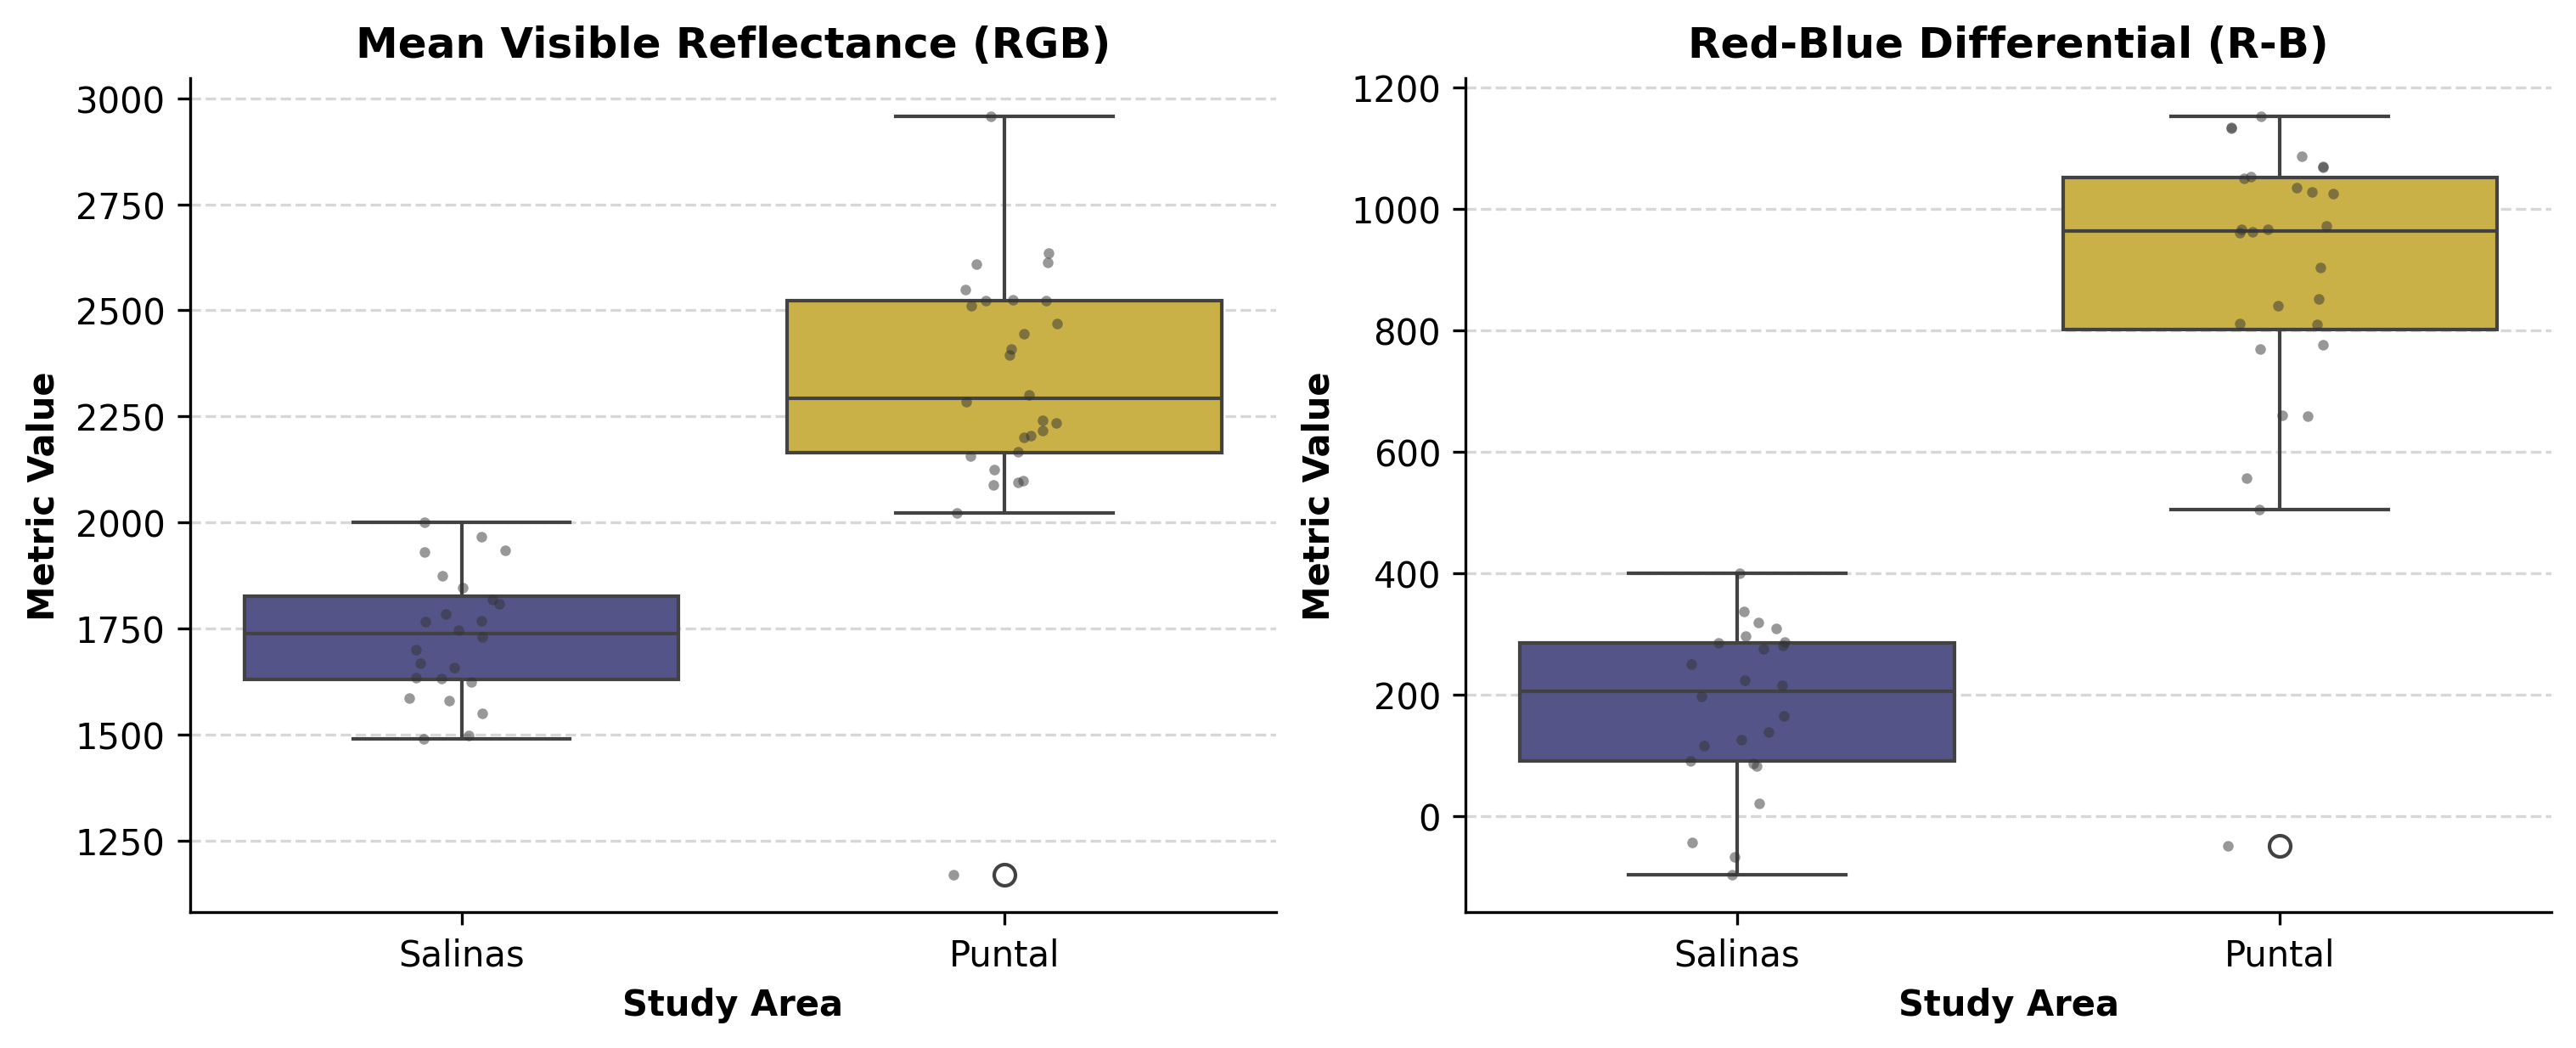
\includegraphics[width=15truecm]{figure_brightness_comparison_by_site.png}
    \caption{Comparison of the sand reflectance metrics between El Puntal and Salinas. The left panel displays the absolute albedo proxy ($\bar{\rho}_{RGB}$), while the right panel highlights the colorimetric slope ($\Delta_{R-B}$). Boxplots represent the interquartile range and median, with overlaid stripplots detailing individual scene observations.}
    \label{fig:reflectance_boxplots}
\end{figure}

% Esta sección sirve para establecer el contexto físico antes de ver cómo fallan los modelos basados en índices espectrales.
% Narrativa: Aquí presentarás las distribuciones probabilísticas (histogramas o KDEs) de \bar{\rho}_{RGB} y \Delta_{R-B} entre Salinas y El Puntal.
% Objetivo: Confirmar la hipótesis de que la arena de Salinas es espectralmente más oscura, sentando la base para entender los fallos.

\section{Deep Learning Pixel-based Performance}
\label{sec:results_pixel_eval}
% Presentación de las métricas puramente basadas en la matriz de píxeles medidas dentro del buffer de 100m.
% Objetivo: Demostrar que las arquitecturas aprendieron correctamente a segmentar la clase "agua" antes del proceso de vectorización subpíxel.

\section{Geometric Evaluation: Cross-shore Offsets}
\label{sec:results_geometric_eval}
% Introducción breve indicando que esta sección traslada el análisis al dominio geométrico (metros) usando la metodología de transectos.

\subsection{Overarching Family Performance (Index-based vs. Deep Learning)}
\label{subsec:overarching_performance}

To establish a macroscopic comparison between the two fundamental approaches, the cross-shore extraction errors (offsets) were initially aggregated by model family across both study areas. Figure \ref{fig:overall_family_boxplots} (left panel) presents the overall performance distributions, revealing a decisive superiority of the Deep Learning architectures over the traditional spectral baselines. 

Globally, the DL-based models achieved a median offset of 5.56 m, nearly halving the 10.02 m median error recorded by the Index-based methods. Beyond the absolute magnitude of the error, the variance showcases an even more critical disparity. The interquartile range (IQR) for the DL family is remarkably tight (7.42 m), whereas the traditional indices exhibit a widespread error distribution (IQR of 21.08 m). This indicates that, regardless of the specific architecture or thresholding technique applied, semantic segmentation models consistently yield highly stable and precise waterline contours, minimizing severe extraction failures.

However, the overarching advantage of the Deep Learning approach becomes most apparent when the error distributions are disaggregated by study area (Figure \ref{fig:overall_family_boxplots}, right panel). This spatial breakdown directly tests the models against the morphological complexities established in Section \ref{sec:results_sand_reflectance}. In Section \ref{subsec:environmental_drivers}, these differences will be further analyzed in detail.

For the Index-based family, the extraction performance is highly site-dependent. At the relatively sheltered, golden-sanded baseline of El Puntal, the indices perform reasonably well, maintaining a median offset of 7.81 m and a relatively controlled 75th percentile (Q3: 16.69 m). In stark contrast, when deployed over the stress-test environment of Salinas, the traditional algorithms experience a severe degradation. The median error completely doubles to 16.32 m, and the distribution stretches massively, with the Q3 reaching 51.79 m. This severe structural downgrade confirms that pixel-by-pixel spectral formulations are fundamentally vulnerable to the radiometric ambiguity caused by dark carbonaceous sand and extensive wave foam.

Conversely, the Deep Learning models demonstrate an outstanding geographic invariance. At El Puntal, the DL family achieves a median error of 5.47 m. When subjected to the challenging conditions of Salinas, the performance remains virtually unchanged, with a median offset of 5.72 m and a strictly bounded upper quartile (Q3: 10.53 m). This remarkable consistency proves that advanced neural networks successfully leverage broader spatial context and structural patterns. By understanding the semantic relationship between the breaking waves, the wet sand, and the ocean, the DL architectures effectively bypass the spectral limitations that severely penalize traditional thresholding techniques in highly dynamic macrotidal environments.

\begin{figure}[H]
    \centering
    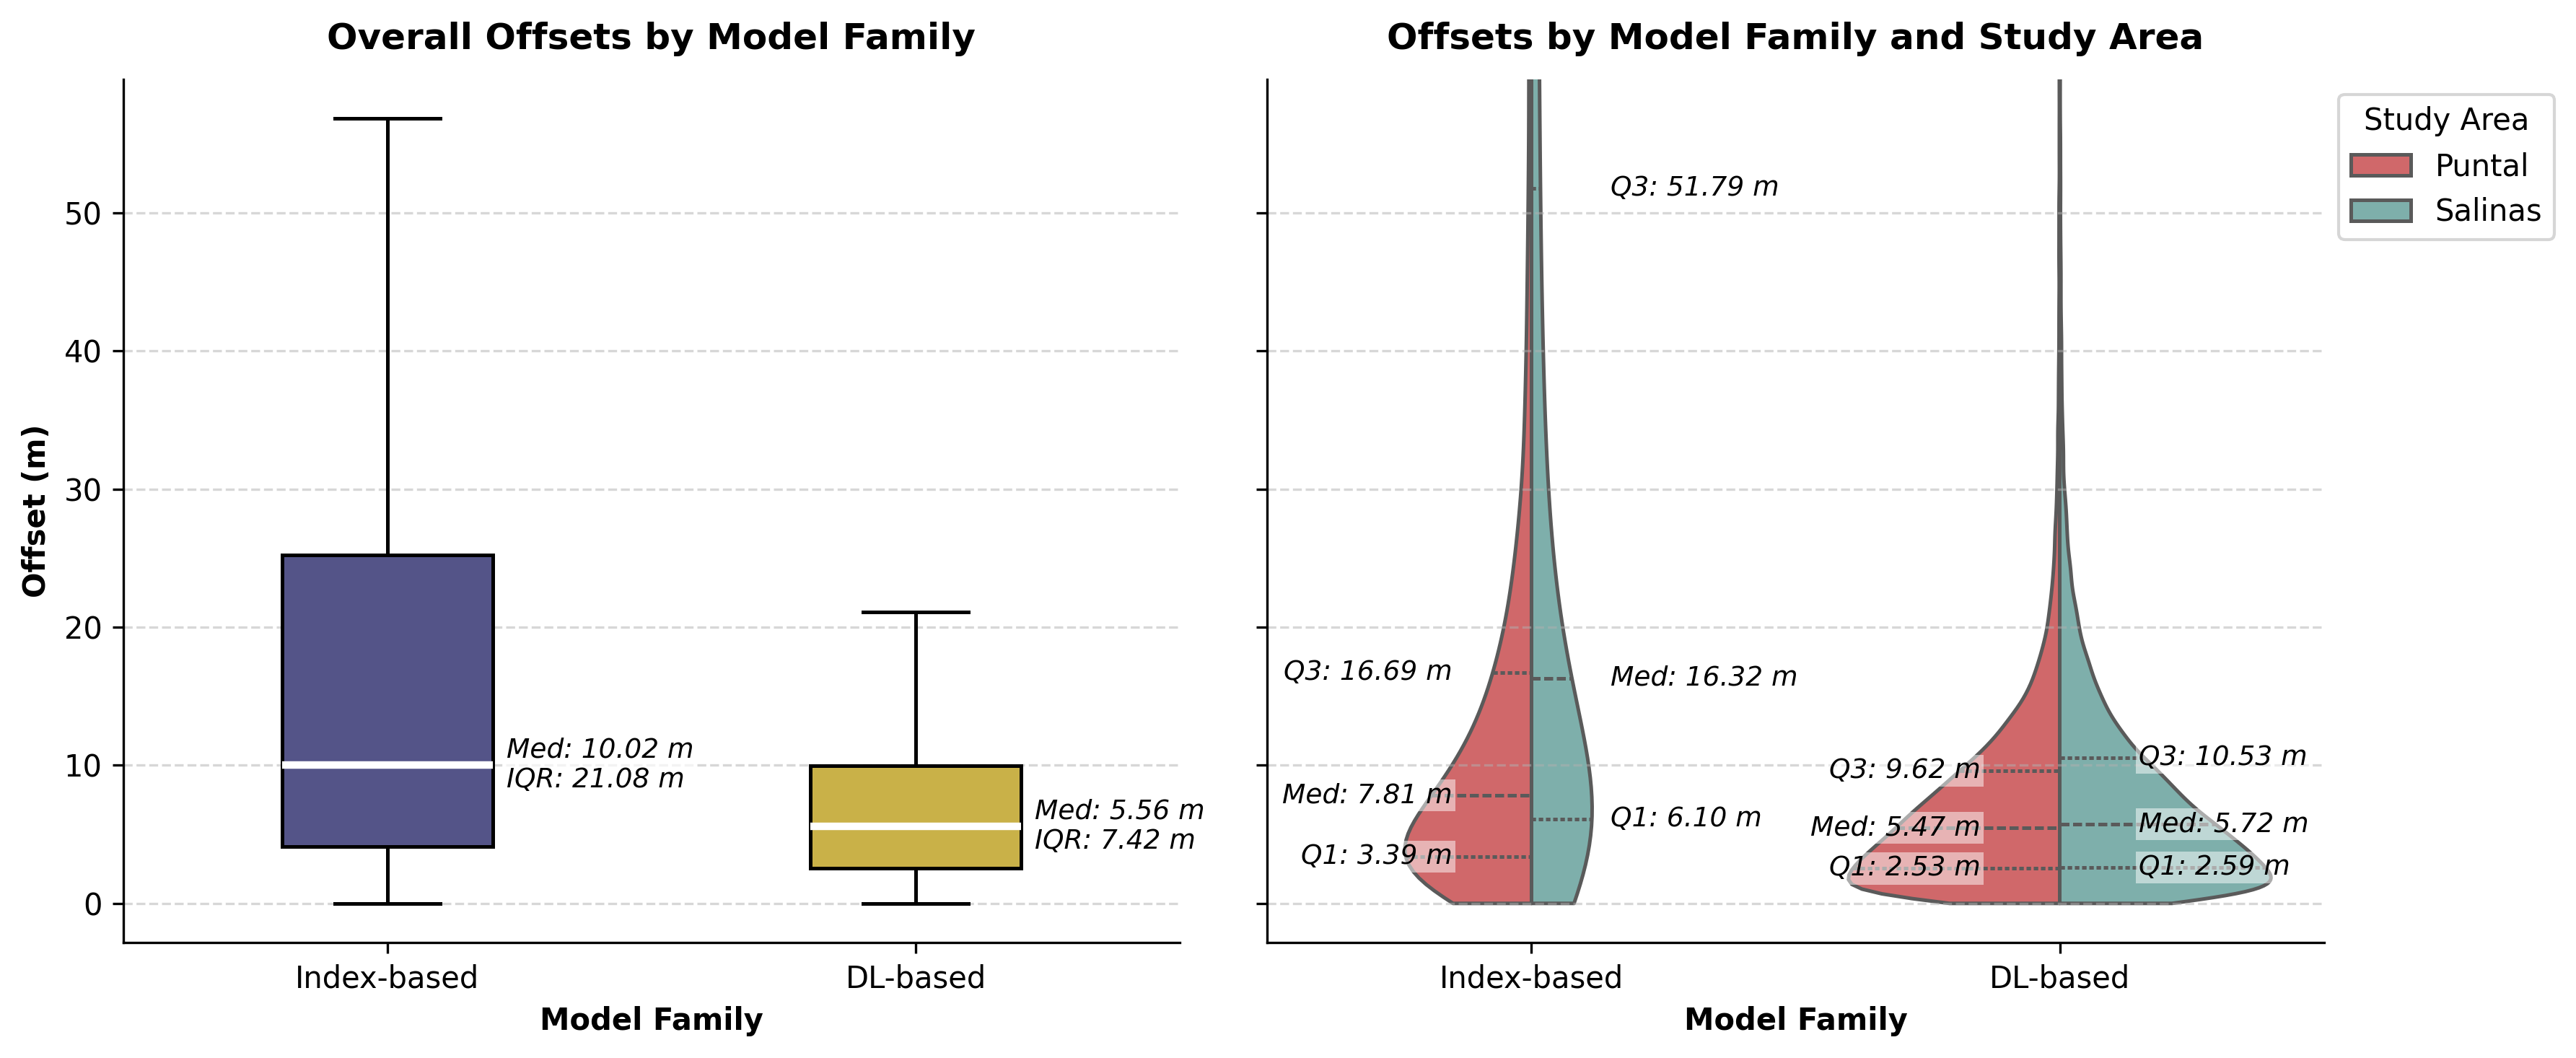
\includegraphics[width=17truecm]{figure_overall_family_boxplots.png}
    \caption{Distribution of cross-shore extraction offsets by model family. The left panel (Boxplot) displays the aggregated global performance, highlighting the median and interquartile range (IQR). The right panel (Violin plot) disaggregates the errors by study area (El Puntal vs. Salinas), emphasizing the severe performance degradation of index-based methods in complex environments compared to the geographic robustness of DL models.}
    \label{fig:overall_family_boxplots}
\end{figure}

% Responde a la Q1: Cuál de los dos grandes mundos algorítmicos tiene menos error absoluto y cuál sufre más dependiendo de la morfología de la playa.
% Gráficos del notebook: El panel doble con el Boxplot general (izquierda) y el Violin plot dividido por playa (derecha).

\subsection{Intra-Family Model Assessment and Spatial Bias}
\label{subsec:intra_family_assessment}

Having established the overarching superiority of the Deep Learning approach, it is necessary to intrinsically evaluate the specific configurations within each family. This intra-family assessment identifies which architectural combinations and thresholding techniques yield the highest predictive power, utilizing the Mean Absolute Error (MAE) as the primary evaluation metric.

% Se destaca la inestabilidad y el buen rendimiento del SCoWI + LM Otsu.
Regarding the Index-based models, the error matrix reveals an extreme sensitivity to the chosen binarization threshold. The performance of a single spectral index can fluctuate drastically depending on the thresholding algorithm applied. For instance, MNDWI suffers a massive degradation using a Zero threshold (MAE: 48.35 m) but improves significantly with the Local Minimum (LM) Otsu (17.34 m). Conversely, NDWI performs reasonably with a Zero cutoff (20.22 m) but completely fails under LM Otsu (48.43 m). Standard Otsu consistently yields poor results across most indices, struggling with the multimodal histograms of macrotidal beaches. Notably, the optimal configuration within this family is the subtractive SCoWI coupled with the LM Otsu threshold, achieving a MAE of 8.71 m. This result empirically validates the SCoWI's specific formulation designed to suppress wave foam and intertidal noise, provided it is paired with a context-aware thresholding technique.

% Se destaca la estabilidad y el éxito de la hibridación (U-Net + MiT-B2).
In stark contrast to the volatility of the traditional indices, the Deep Learning matrix exhibits remarkable algorithmic stability. Regardless of the architecture or encoder chosen, all DL configurations constrained their average error to a tight operational band between 7.27 m and 8.54 m. Within this high-performing group, the U-Net architecture consistently outperformed SegFormer and DeepLabV3+. Most importantly, the results confirm the hybridization hypothesis proposed in the methodological framework (Section \ref{sec:dl_models}). Combining the global-context awareness of the hierarchical Vision Transformers (MiT-B2 and MiT-B4) into the precise local-feature CNN decoder of U-Net yielded the absolute best global performance. Specifically, the U-Net paired with the MiT-B2 encoder achieved the lowest recorded error of the entire study, with a MAE of 7.27 m. Interestingly, a nuanced pattern emerges in this matrix regarding model capacity and feature extraction depth. With the exception of DeepLabV3+, which marginally benefited from increased parameterization, both the U-Net and SegFormer architectures systematically yielded better geometric accuracy when paired with lighter encoders, such as EfficientNet-B4 and MiT-B2, rather than heavier, more complex counterparts, such as EfficientNet-B7 and MiT-B4. This suggests that excessively deep encoders may induce a degree of spatial overfitting or loss of the high-resolution features necessary for precise shoreline delineation, particularly in the context of the complex coastal environments evaluated in this study.

\begin{figure}[H]
    \centering
    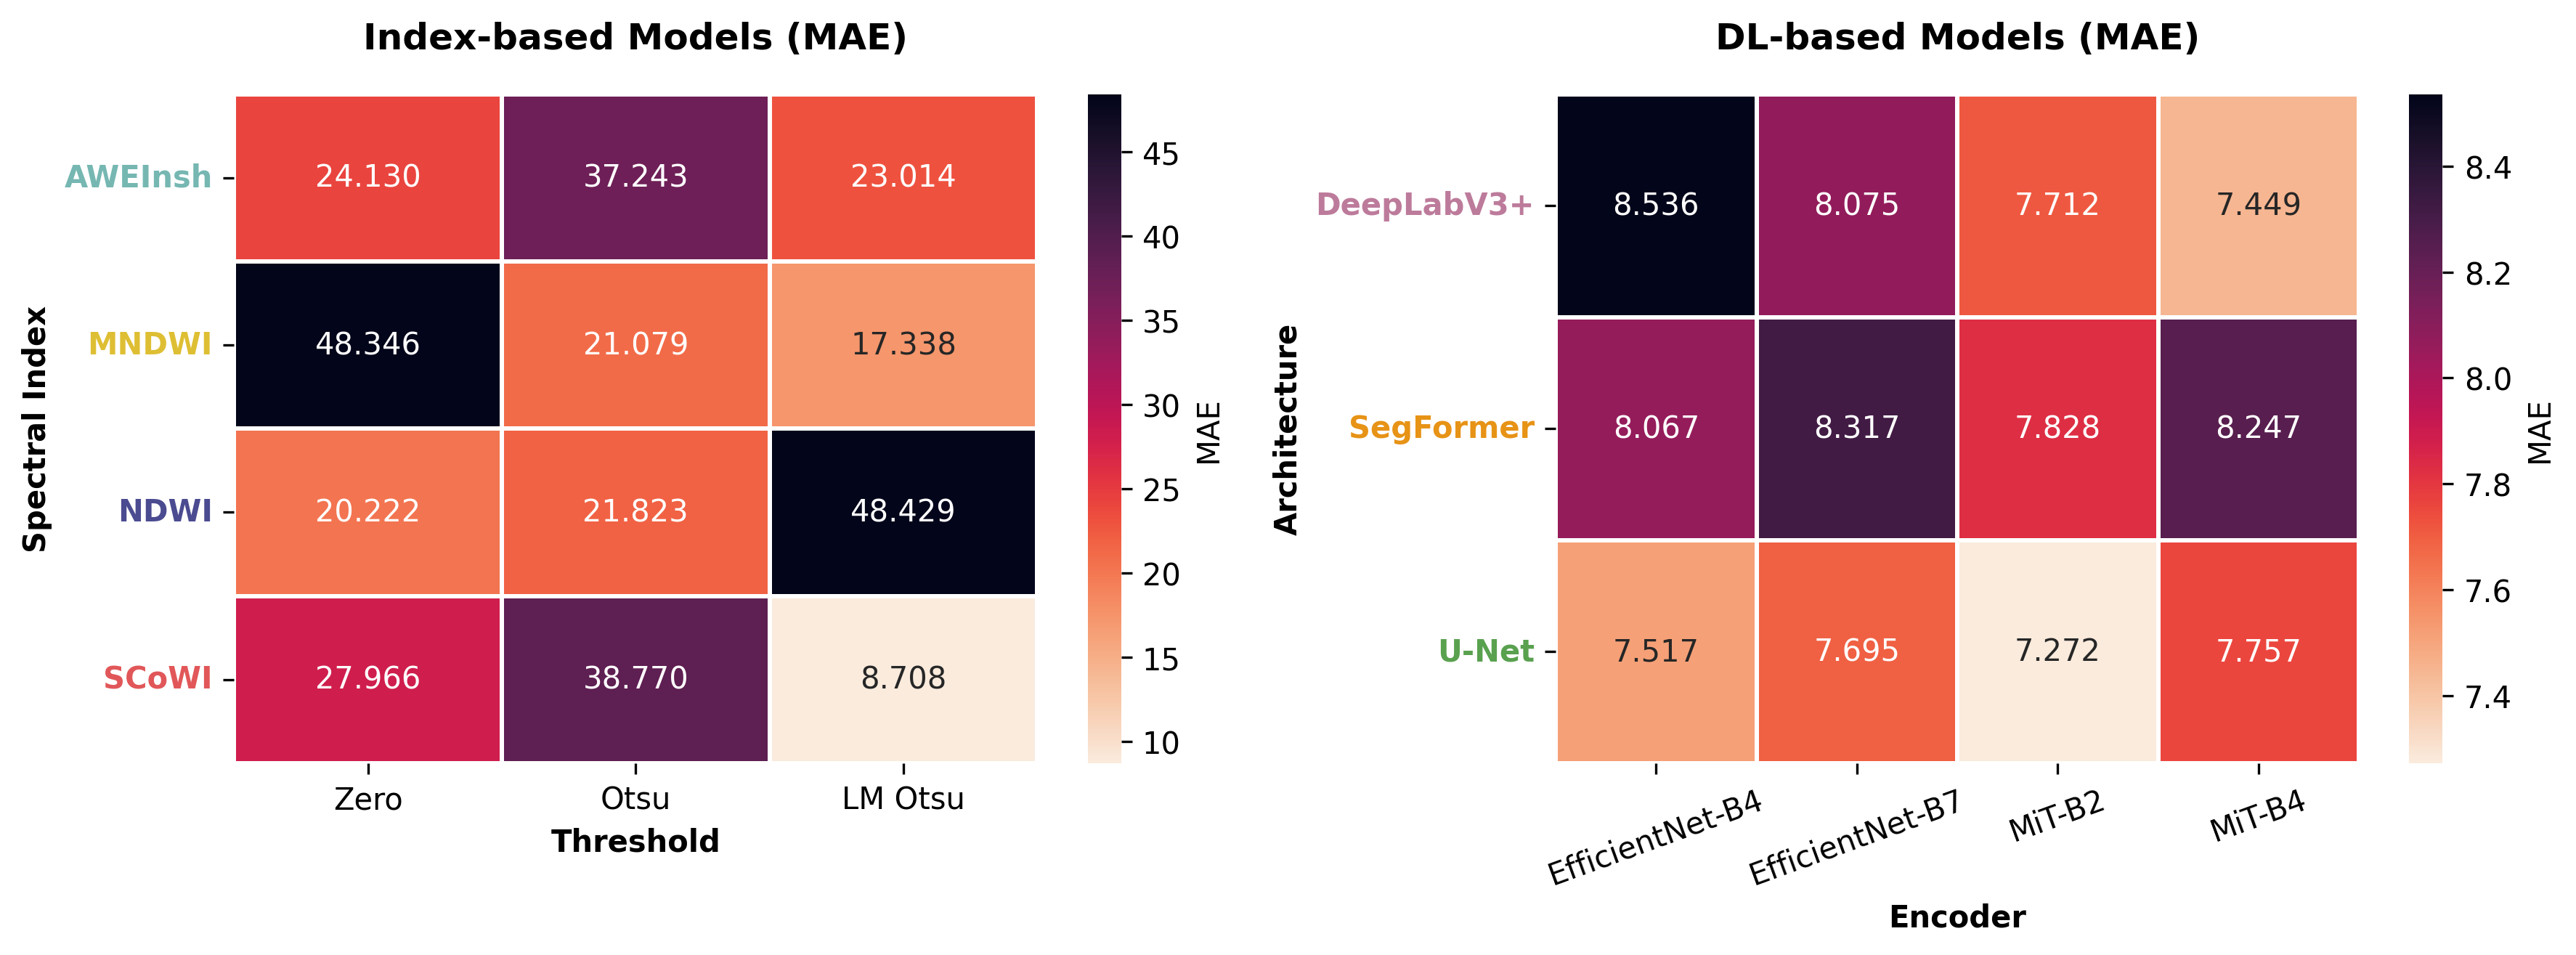
\includegraphics[width=\textwidth]{figure_heatmap_mae.png}
    \caption{Mean Absolute Error (MAE) heatmaps for intra-family configuration assessment. The left panel details the performance of spectral indices across different thresholding techniques, highlighting extreme variance. The right panel displays the Deep Learning configurations, demonstrating high stability and the superiority of the U-Net (MiT-B2) hybrid architecture.}
    \label{fig:mae_heatmaps}
\end{figure}

% Frase de transición hacia la segunda mitad de la sección (Hexbins).
Beyond the absolute magnitude of the extraction error, it is critical for coastal engineering applications to understand the orientation of this displacement. To assess whether the models exhibit a systematic spatial bias (tending to delineate the waterline either too far inland or too far seaward), the cross-shore predictions (SDW) were mapped against the ground-truth reference (RWL) using hexbin density plots.

The hexbin distributions for traditional spectral indices (Figure \ref{fig:hexbins_index}) reveal extreme spatial dispersion and distinct systematic failure modes. The Coefficient of Determination ($R^2$) reflects this volatility, ranging from a low 0.31 (MNDWI Zero) to a highly correlated 0.91 (SCoWI LM Otsu). Visually, the vast majority of spectral combinations exhibit a pronounced \textit{Landward} bias, characterized by large negative Mean Error (Bias) values. For instance, MNDWI (Zero) and AWEInsh (Otsu) yielded biases of -47.87 m and -33.49 m, respectively. This severe landward offset demonstrates that standard indices systematically misclassify the saturated intertidal zone as water, effectively tracing the boundary between dry and wet sand rather than the true instantaneous waterline. 

Conversely, NDWI (particularly when coupled with LM Otsu) exhibits an extreme \textit{Seaward} bias, recording a massive positive displacement of +46.18 m. This behavior aligns with the well documented vulnerability of the NDWI to breaking wave foam, causing the algorithm to falsely track the outer edge of the surf zone instead of the shoreline. The only robust exception within this traditional family is SCoWI (LM Otsu). It successfully clusters the bulk of its predictions along the 1:1 agreement bisector, achieving an $R^2$ of 0.91 and a minimal landward bias of -2.75 m.

In stark contrast, the hexbin density plots for the Deep Learning models (Figure \ref{fig:hexbins_dl}) display very little spatial dispersion, visually confirming their structural robustness. The visual uniformity across the panels is supported by all evaluated DL configurations achieving a very high $R^2 \ge 0.96$, tightly positioning on the 1:1 bisector line. Unlike the index-based methods, the semantic segmentation architectures completely eliminate the severe landward (wet sand) and seaward (foam) failure modes. 

The statistical metrics reveal a highly controlled, very slight \textit{Seaward} bias across all DL architectures, ranging narrowly from +3.20 m (DeepLabV3+ EfficientNet-B4) to +5.48 m (SegFormer MiT-B4). This indicates a minimal, systematic tendency of the DL models to delineate the waterline marginally closer to the swash zone, in contrast to the traditional baseline with its massive errors. Ultimately, the visual and statistical indistinguishability among the DL hexbins reaffirms that these neural networks have successfully learned the underlying semantic context of the coastal boundary, effectively rendering the extraction process immune to the spectral noise of macrotidal environments.

\begin{figure}[H]
    \centering
    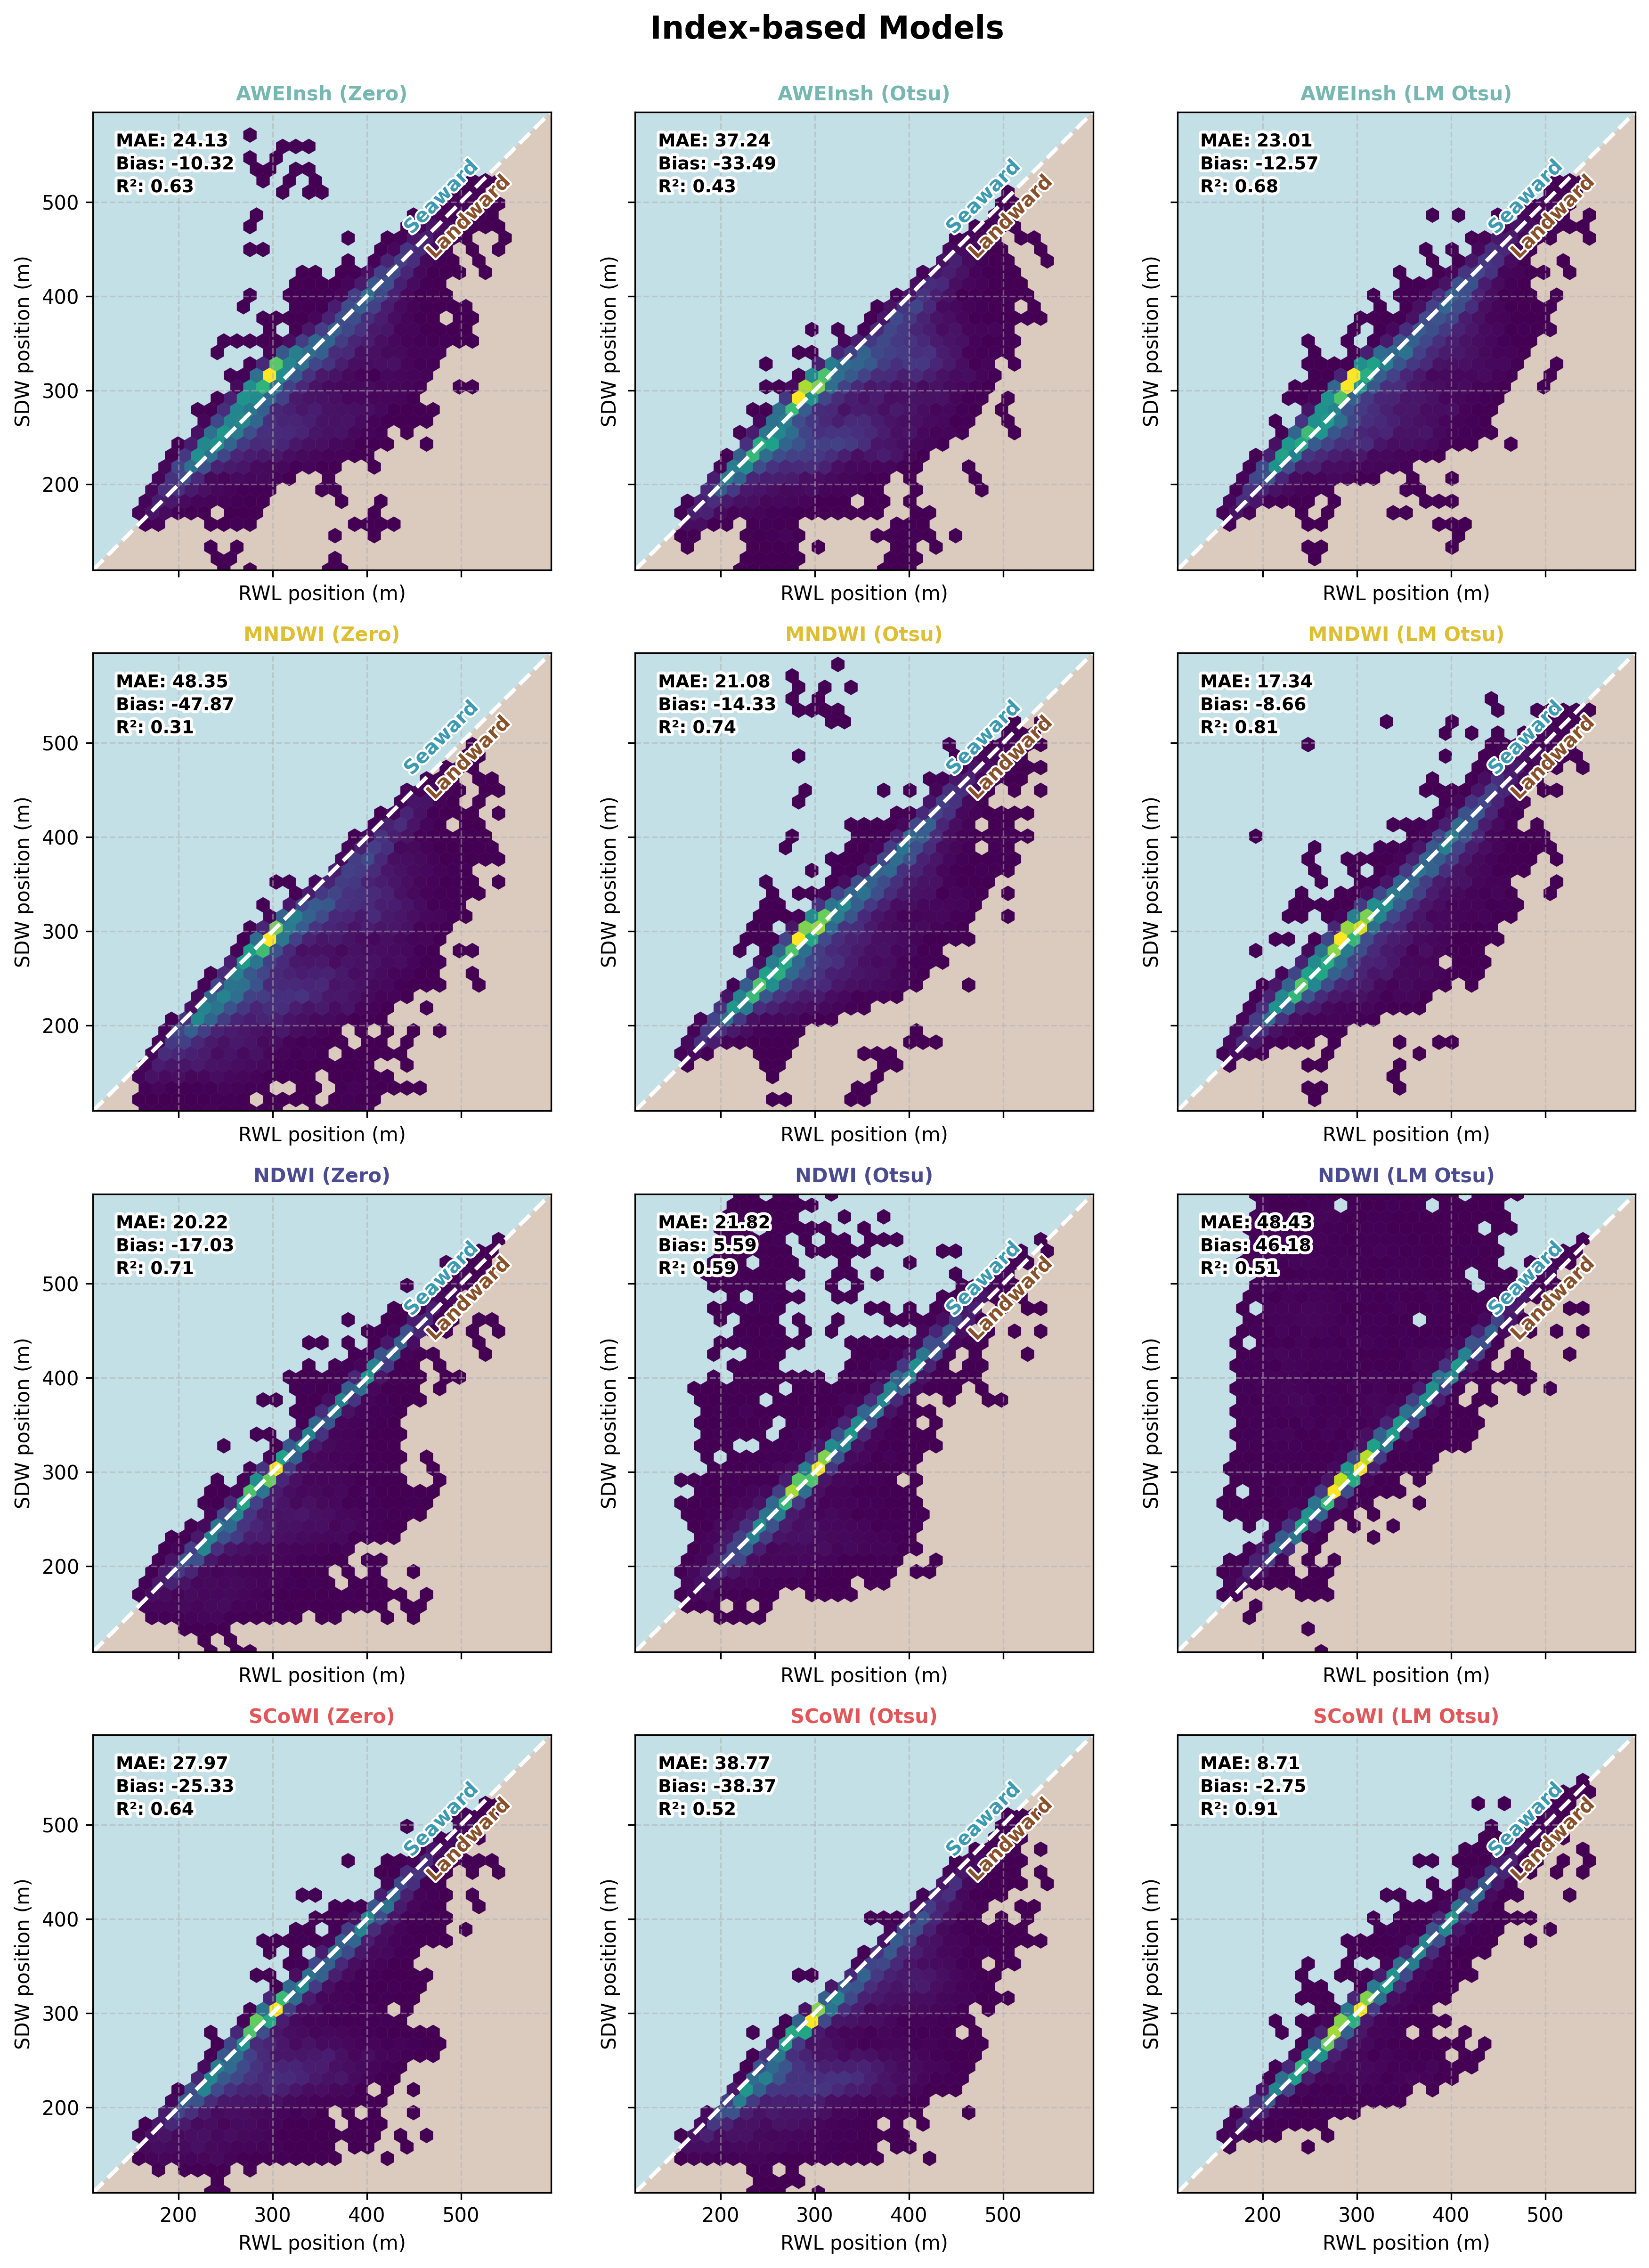
\includegraphics[width=14.5cm]{figure_hexbin_index_models.png}
    \caption{Hexbin error distributions for Index-based models. The plots map the predicted shoreline position (SDW) against the reference waterline (RWL). The dashed white line represents the 1:1 perfect agreement. Most indices show a severe Landward bias (wet sand confusion), while NDWI shows a Seaward bias (foam confusion). SCoWI (LM Otsu) stands out as the most accurate traditional method.}
    \label{fig:hexbins_index}
\end{figure}

\begin{landscape}
    \begin{figure}[p]
        \centering
        % Usar \linewidth asegura que la figura ocupe el ancho máximo de la página apaisada
        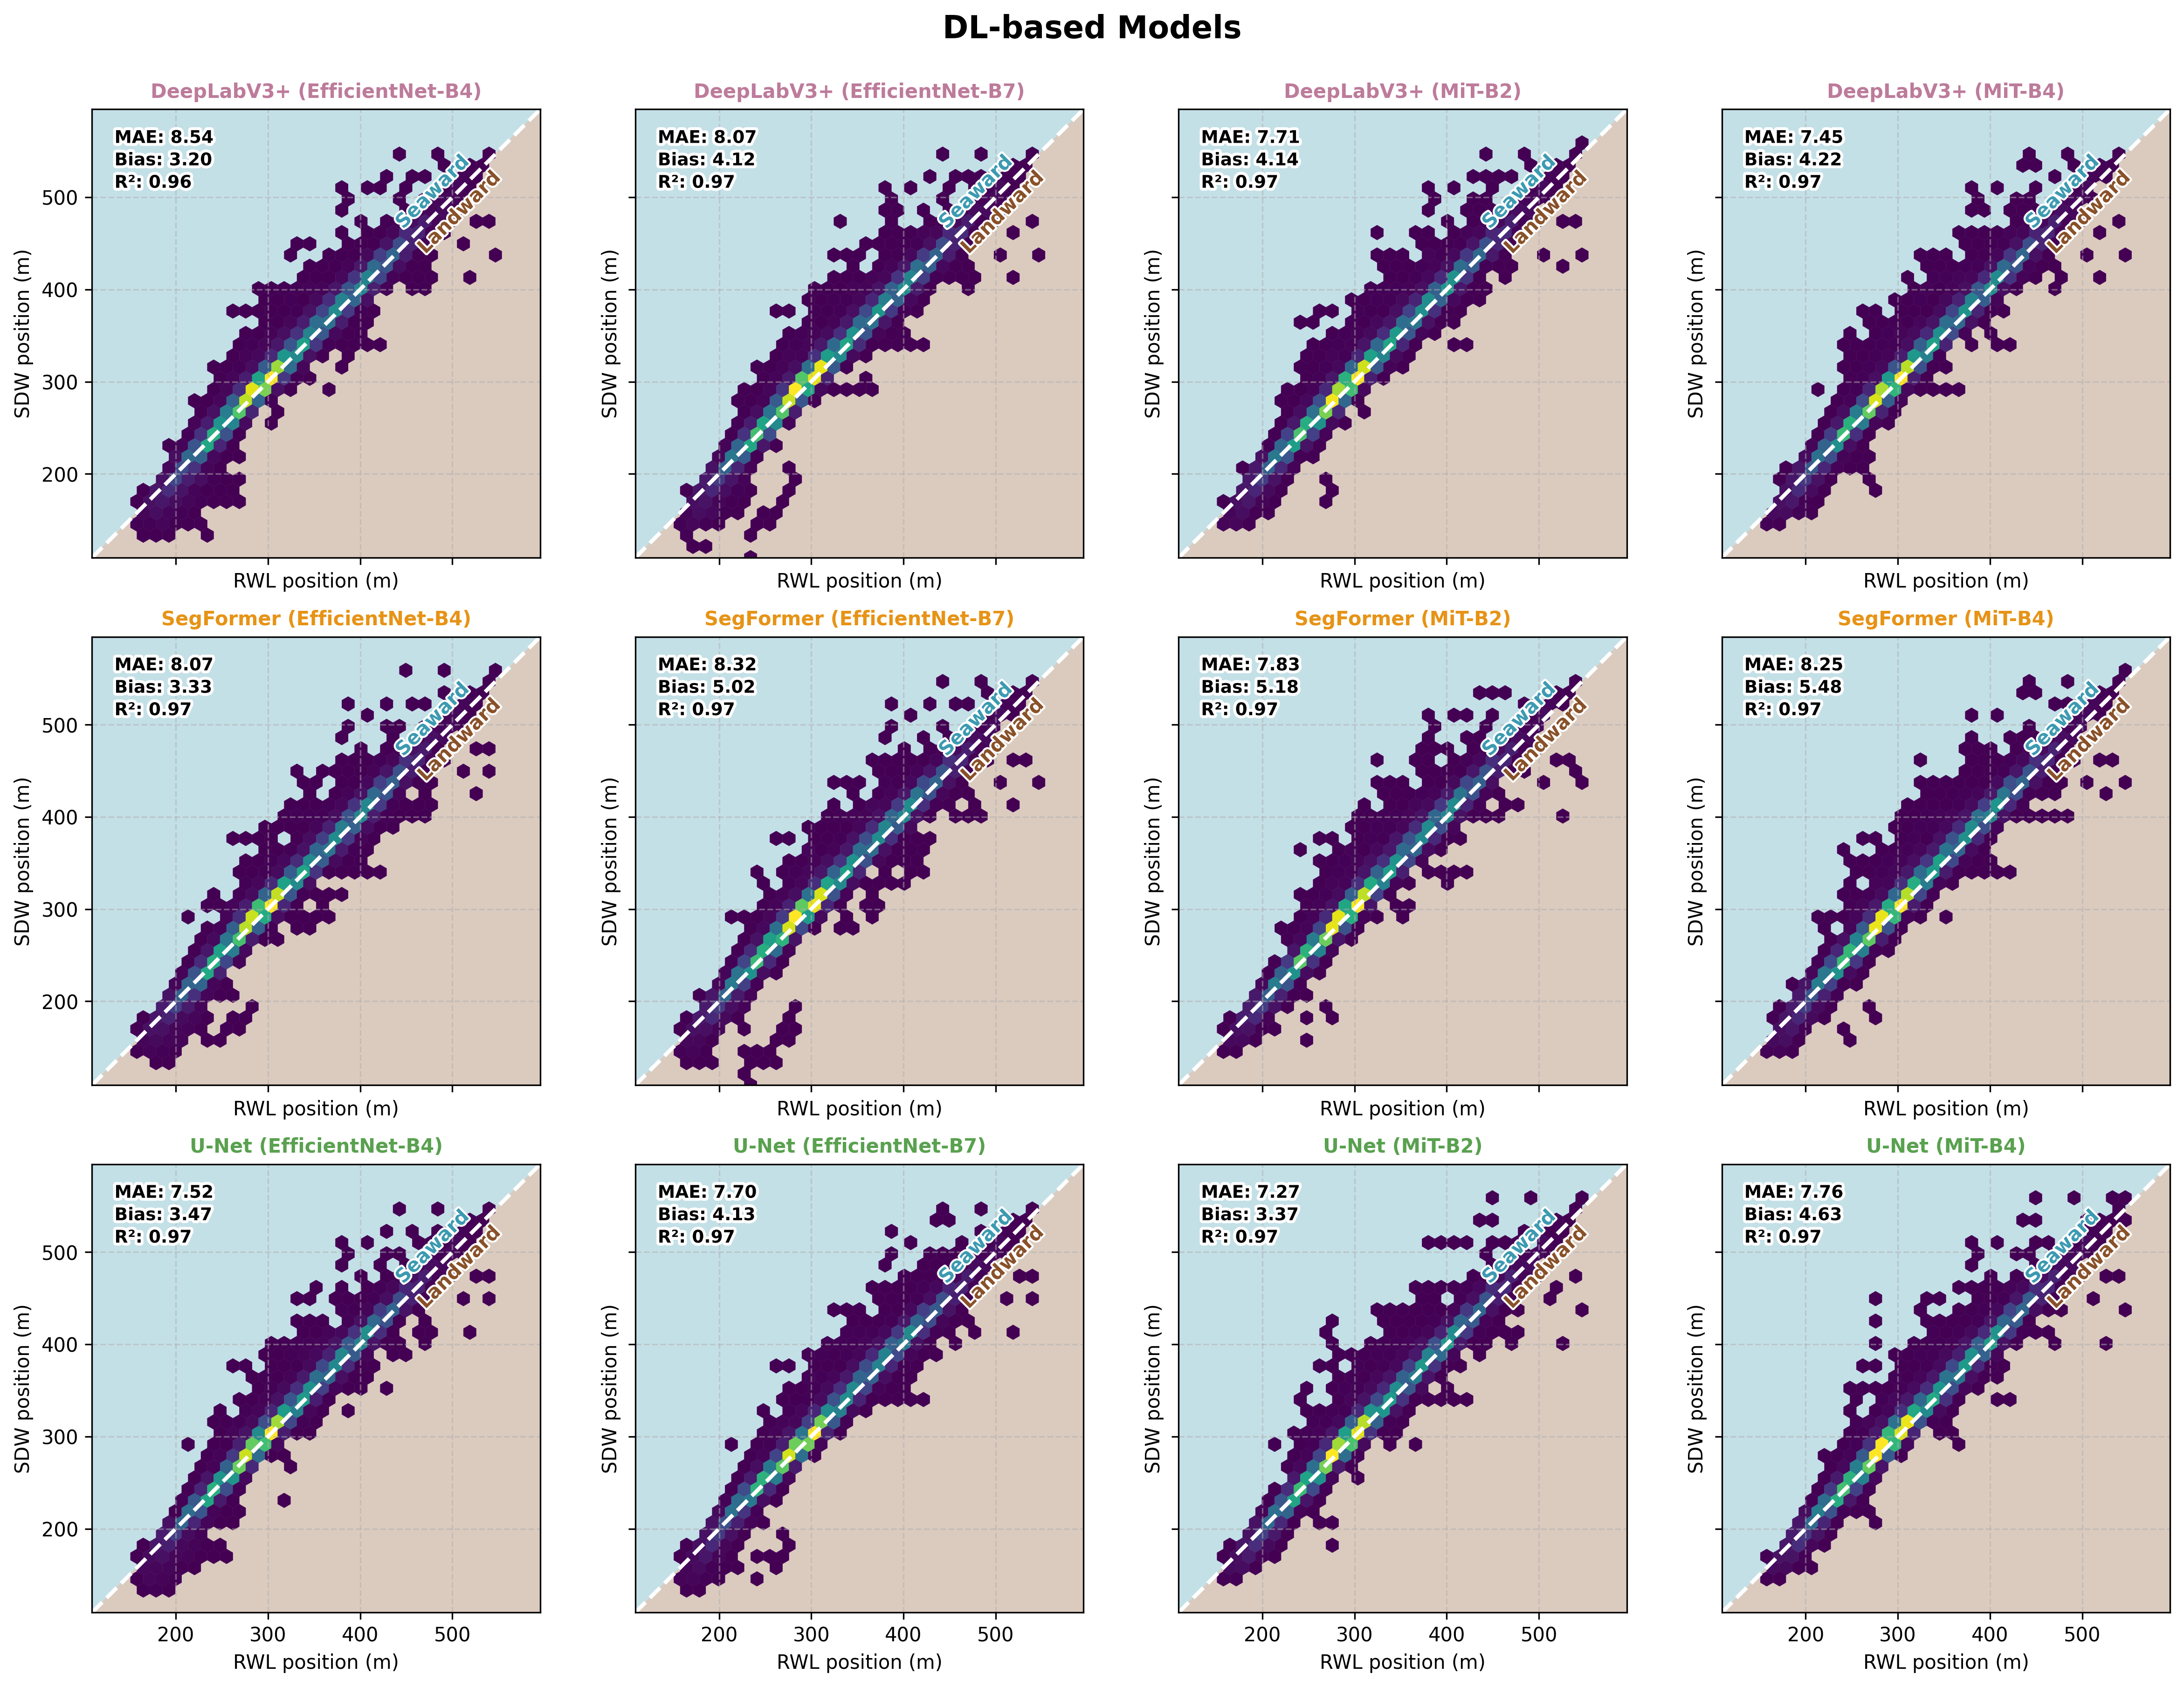
\includegraphics[width=20cm]{figure_hexbin_dl_models.png} 
        \caption{Hexbin error distributions for Deep Learning semantic segmentation models. In contrast to the traditional baseline, all DL configurations demonstrate minimal dispersion, uniformly tight clustering around the 1:1 bisector ($R^2 \ge 0.96$), and the complete elimination of extreme cross-shore biases.}
        \label{fig:hexbins_dl}
    \end{figure}
\end{landscape}

% Responde a la Q2: Evalúa los modelos intrínsecamente y mapea la orientación exacta del error.
% Gráficos del notebook: 
% 1. Los Heatmaps de MAE separados por familias (Thresholds vs Índices y Encoders vs Arquitecturas).
% 2. Los paneles de Hexbins con la línea 1:1, mostrando si los modelos tienden al sesgo Landward (hacia la tierra) o Seaward.

\subsection{Environmental Drivers of Error Variability}
\label{subsec:environmental_drivers}

% Introducción al análisis a lo largo de la costa (alongshore).
Before evaluating the temporal and hydrodynamic forcing, it is essential to examine the spatial variability of the extraction error along the coastline. By analyzing the distribution of cross-shore offsets grouped by \texttt{transect\_id}, specific morphological, geological, or anthropogenic features that locally disrupt model performance can be identified.

% Análisis de los modelos Index-based (Puntal y Salinas).
Figure \ref{fig:transects_index} details this alongshore variability for the Index-based models. At El Puntal, a distinct spatial pattern emerges: the first 15 transects exhibit error metrics (median, third quartile, and maximum bounds) notably below the overall site average. This localized increase in accuracy is driven by two main factors. First, the initial $\approx8$ transects correspond to the navigation channel of the Santander Bay, an area subjected to periodic dredging operations. Second, this entire initial stretch is highly sheltered from incident wave energy, minimizing foam-induced spectral noise. From transect 15 onwards, the offsets closely align with the overall median, until the final 5 transects, where a sudden spike in error is recorded. This localized degradation coincides with a slight shift in the coastline orientation and the proximity to a small stream mouth, which likely introduces spectral confusion due to localized moisture and sediment discharge.

At Salinas, the traditional spectral indices also display significant alongshore volatility. The initial transects record lower-than-average offsets; this physically corresponds to the narrowest sector of the beach where high tides frequently inundate the entire dry sand area, paradoxically restricting the physical space for the models to commit severe landward misclassifications. Conversely, a distinct cluster of elevated errors emerges between transects 12 and 21. This specific coastal stretch is backed by high-rise urban infrastructure. During the Sentinel-2 mid-morning overpass, these buildings project prominent shadows across the intertidal zone, severely confusing the pixel-by-pixel radiometric thresholding of traditional indices. Finally, the last two transects, located immediately adjacent to the eastern inlet jetty, show reduced offsets, likely due to the constrained morphodynamic mobility of the sand volume trapped against this rigid coastal structure.

% Análisis de los modelos DL-based. Destacamos la estabilidad y el pequeño detalle del dique al final.
In sharp contrast to the baseline, the spatial variability across transects for the Deep Learning models (Figure \ref{fig:transects_dl}) is remarkably lower, visually corroborating their geographic robustness. At El Puntal, there is a marginal reduction in offsets between transects 3 and 10, but the magnitude of this variation is virtually negligible compared to the volatility of the index-based models. Similarly, at Salinas, the DL predictions remain stable across the entire beach longitude, effectively bypassing the severe urban shadow artifacts seen in spectral indices. The only notable, albeit minor, anomaly occurs in the last four transects near the Salinas jetty. Here, the DL models register slightly higher offsets relative to their internal overall median.

% --- Figura de Transectos: Index-based ---
\begin{figure}[H]
    \centering
    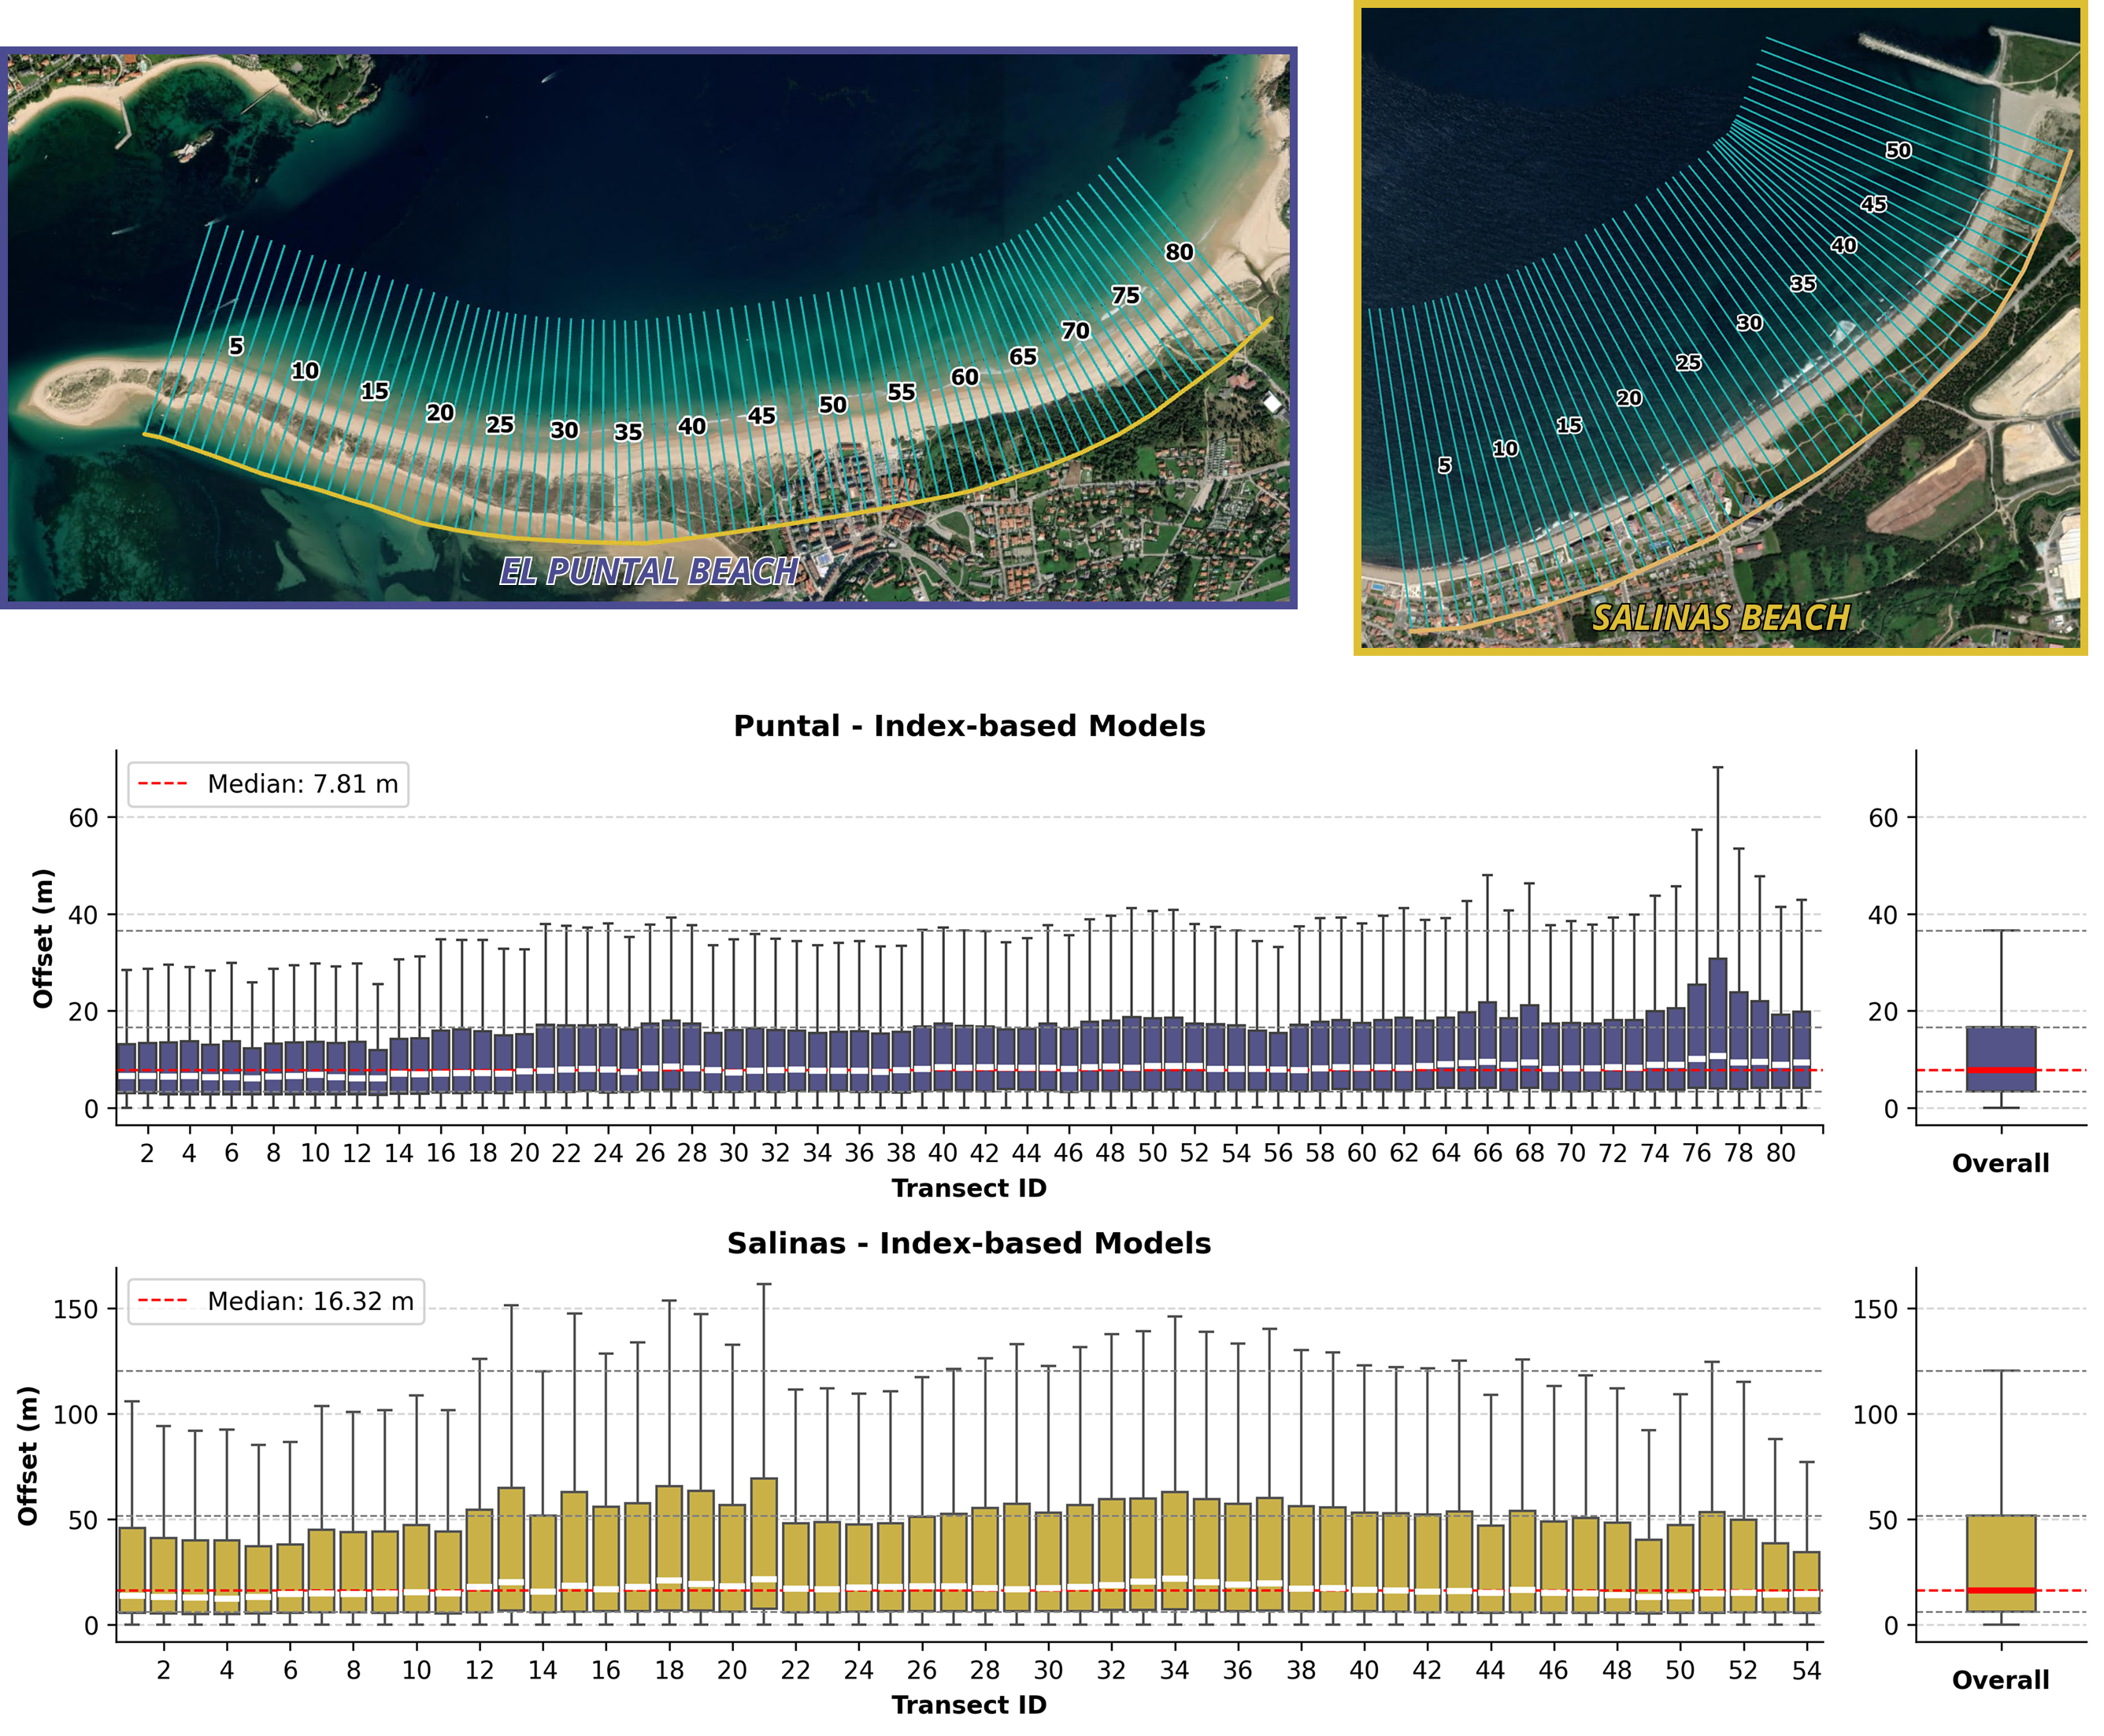
\includegraphics[width=\textwidth]{figure_boxplot_by_transect_index_models_with_map.png}
    \caption{Alongshore variability of extraction offsets for Index-based models. The upper map panels reference the geographical location of the cross-shore transects. The boxplots show the error distribution per \texttt{transect\_id} compared to the overall site performance (right sub-panels).}
    \label{fig:transects_index}
\end{figure}

% --- Figura de Transectos: DL-based ---
\begin{figure}[H]
    \centering
    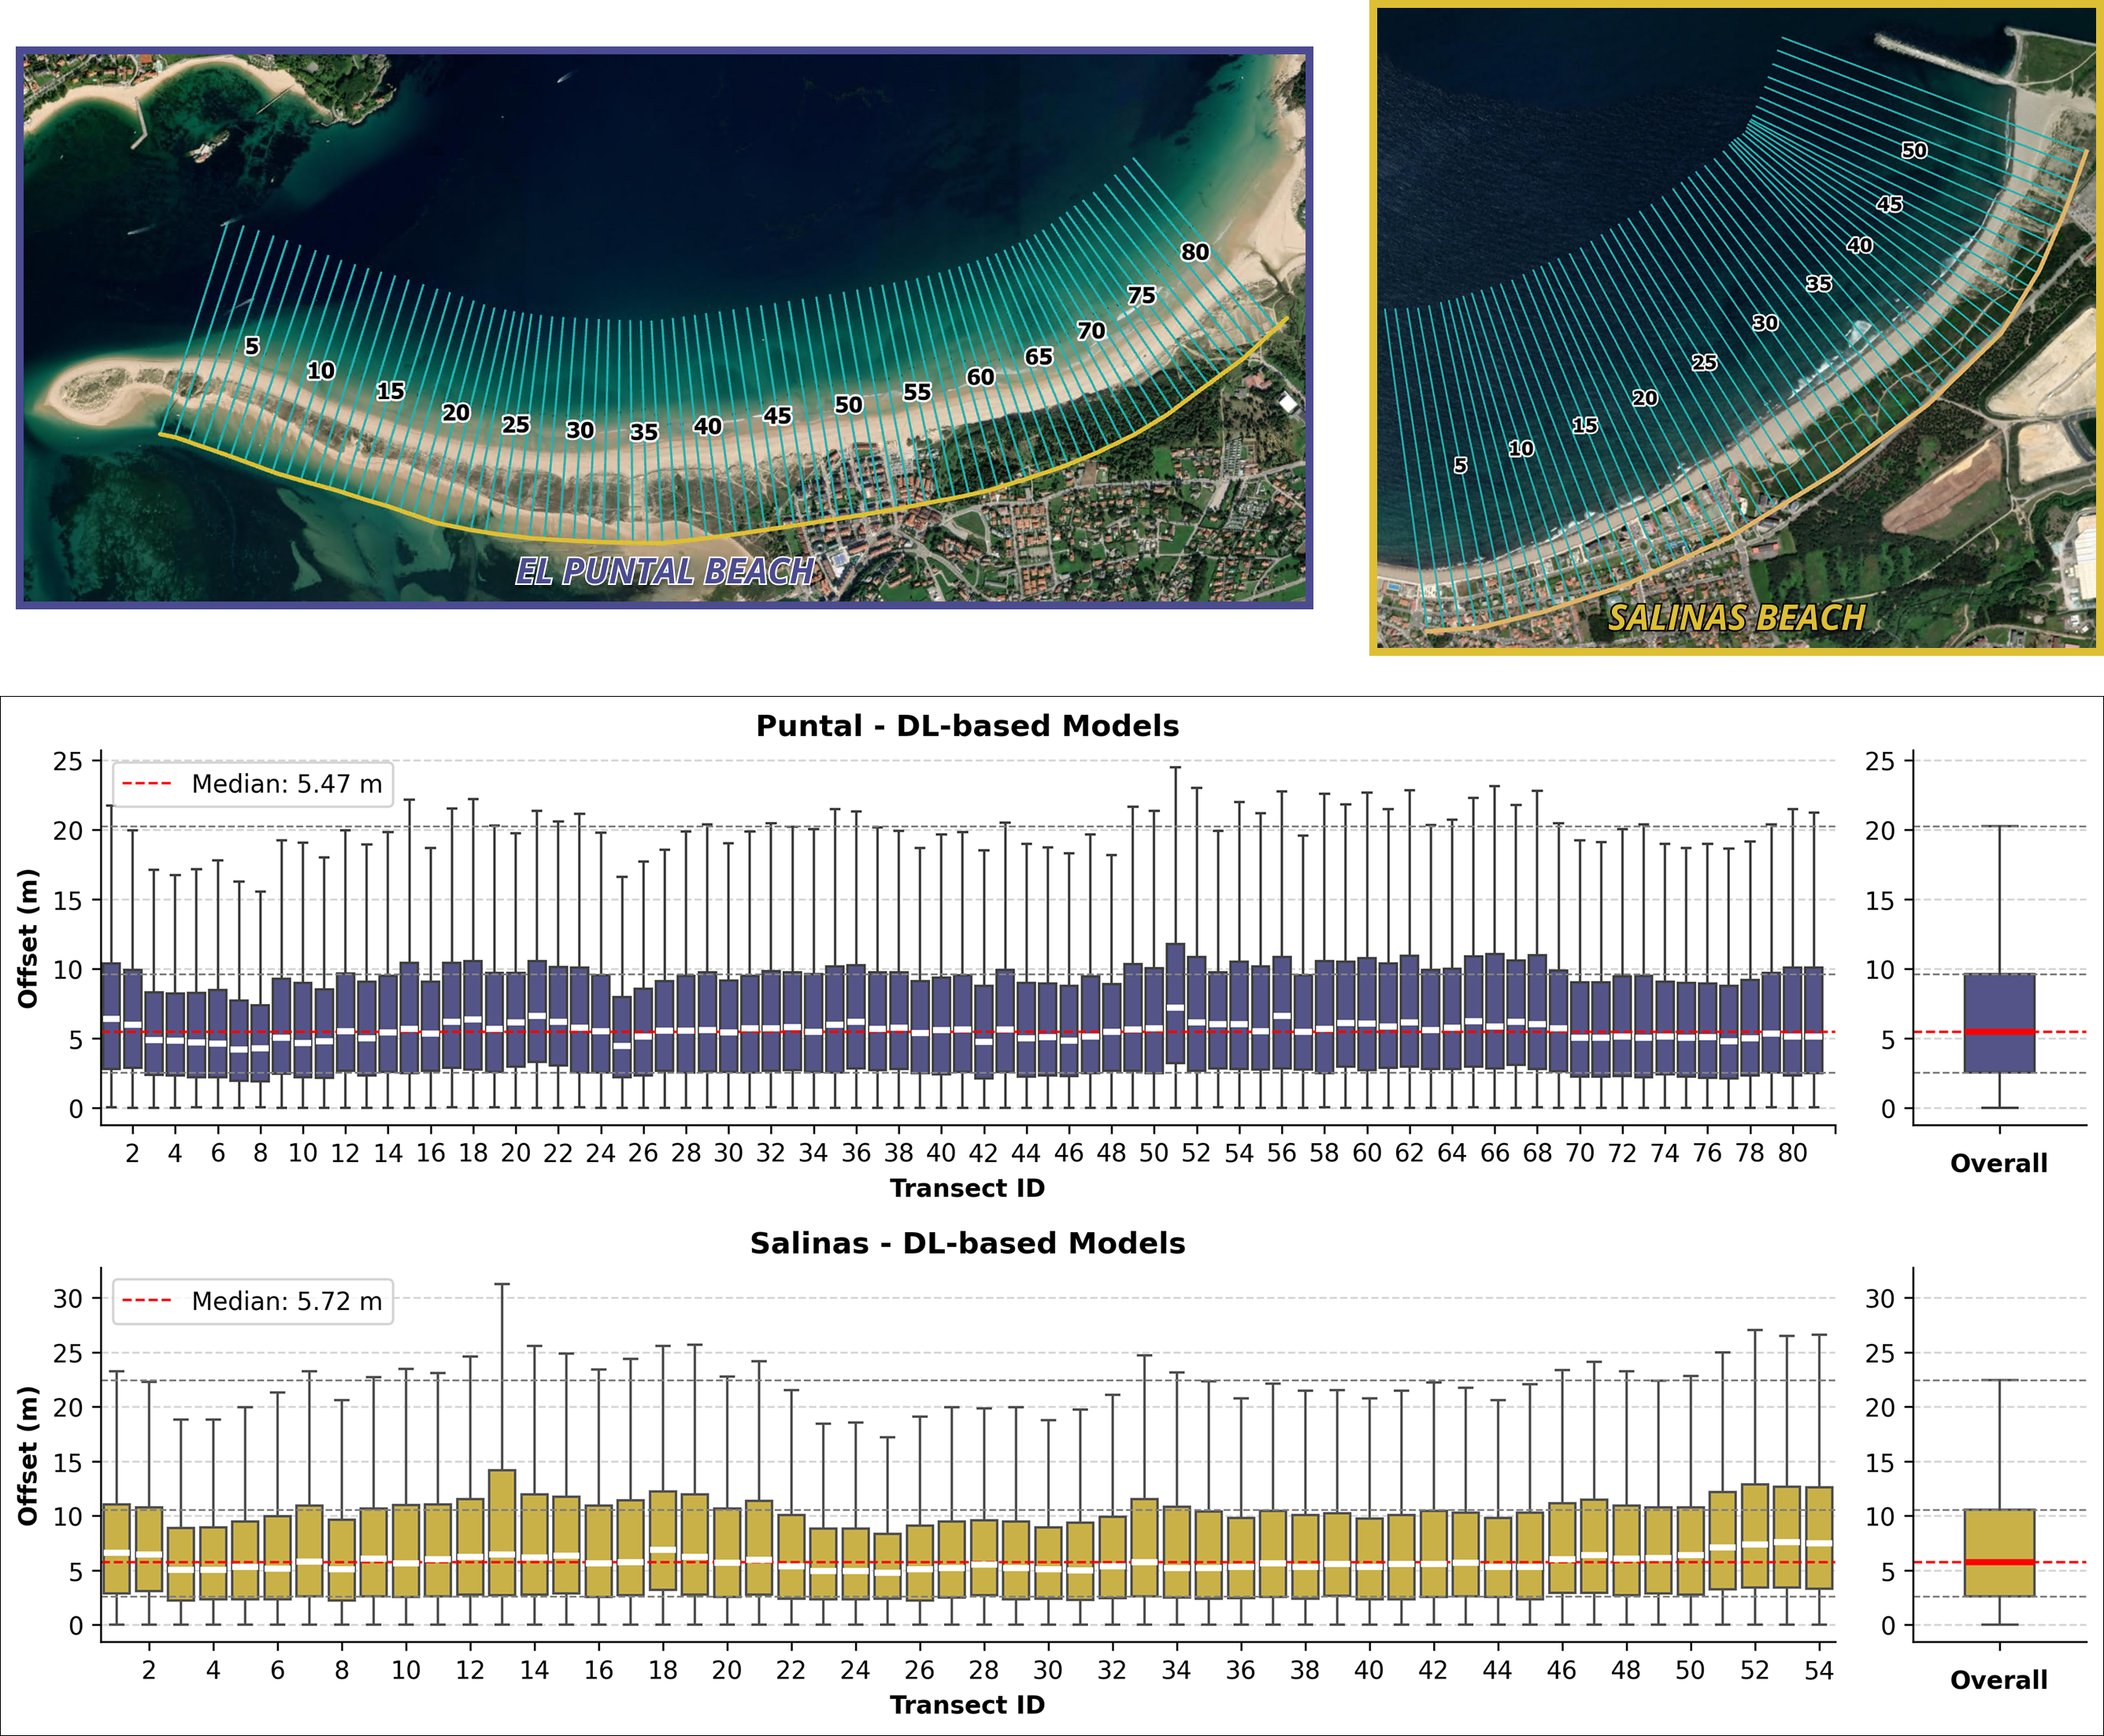
\includegraphics[width=\textwidth]{figure_boxplot_by_transect_dl_models_with_map.png}
    \caption{Alongshore variability of extraction offsets for Deep Learning models. The upper map panels reference the geographical location of the cross-shore transects. The boxplots show the error distribution per \texttt{transect\_id} compared to the overall site performance (right sub-panels).}
    \label{fig:transects_dl}
\end{figure}

% Este texto cierra la sección 4.3.3. Empieza explicando cómo medimos la influencia hidrodinámica (con porcentajes) y luego ataca Marea y Oleaje.

Beyond spatial artifacts, the temporal variability forced by hydrodynamic conditions, specifically astronomical tide and significant wave height ($H_s$) was evaluated. To isolate the environmental sensitivity of the models from their baseline errors, the performance was analyzed using the relative percentage change ($\Delta \%$) of the offset within each hydrodynamic quartile against the overall median of each specific study site.

The tide quartile analysis reveals a critical, structurally consistent phenomenon: the lowest performance across all models occurs during low tide (Q1), rather than high tide (Q4). For the Index-based models, this degradation is catastrophic in the Salinas stress-test environment, where the Q1 relative offset spikes by +312.9\% (reaching an absolute median error of 67.38 m). Physically, low tide in macrotidal beaches exposes a vast intertidal zone characterized by water-saturated sand, complex rhythmic forms, and remnant pooling. This flat, dark, and highly reflective wetted surface critically confuses pixel-based thresholding algorithms. Conversely, during high tide (Q4), the complex intertidal zone is entirely submerged, leaving a starker dry sand-water boundary that improves the index-based relative performance by -51.6\% in Salinas and -22.0\% in El Puntal.

The Deep Learning models exhibit a conceptually similar sensitivity profile to the tidal cycle, confirming that the exposure of the intertidal zone is an inherently challenging feature even for human annotators. However, the magnitude of their sensitivity is exceptionally controlled. In Salinas, the DL Q1 relative downgrade is only +30.2\%, which translates to a highly operational absolute median offset of just 7.44 m. This demonstrates that while the neural networks detect the physical ambiguity of the wet sand, their spatial context awareness prevents the catastrophic delineations that plague traditional indices.

Regarding wave energy forcing, a direct correlation between significant wave height ($H_s$) and extraction error is observed. For the Index-based models, transitioning from calm seas (Q1) to storm conditions (Q4) steadily increases the relative error in both El Puntal (from -7.0\% to +16.9\%) and Salinas (from -16.5\% to +25.0\%). This deterioration is a direct consequence of extensive white water foam and wave run-up physically widening the swash zone, which the spectral indices misclassify. 

The DL-based architectures once again demonstrate superior resilience against wave forcing. At El Puntal, the models remain completely stable regardless of the wave height, fluctuating minimally. In Salinas, the onset of extreme wave conditions (Q4) induces a slight relative increase of +18.0\%. Nevertheless, this relative bump corresponds to an absolute median error of only 6.74 m, confirming that the semantic segmentation networks can accurately track the underlying shoreline position regardless of extreme surf zone hydrodynamics.

% --- Figura de los Cuartiles Hidrodinámicos (Relativo) ---
\begin{figure}[H]
    \centering
    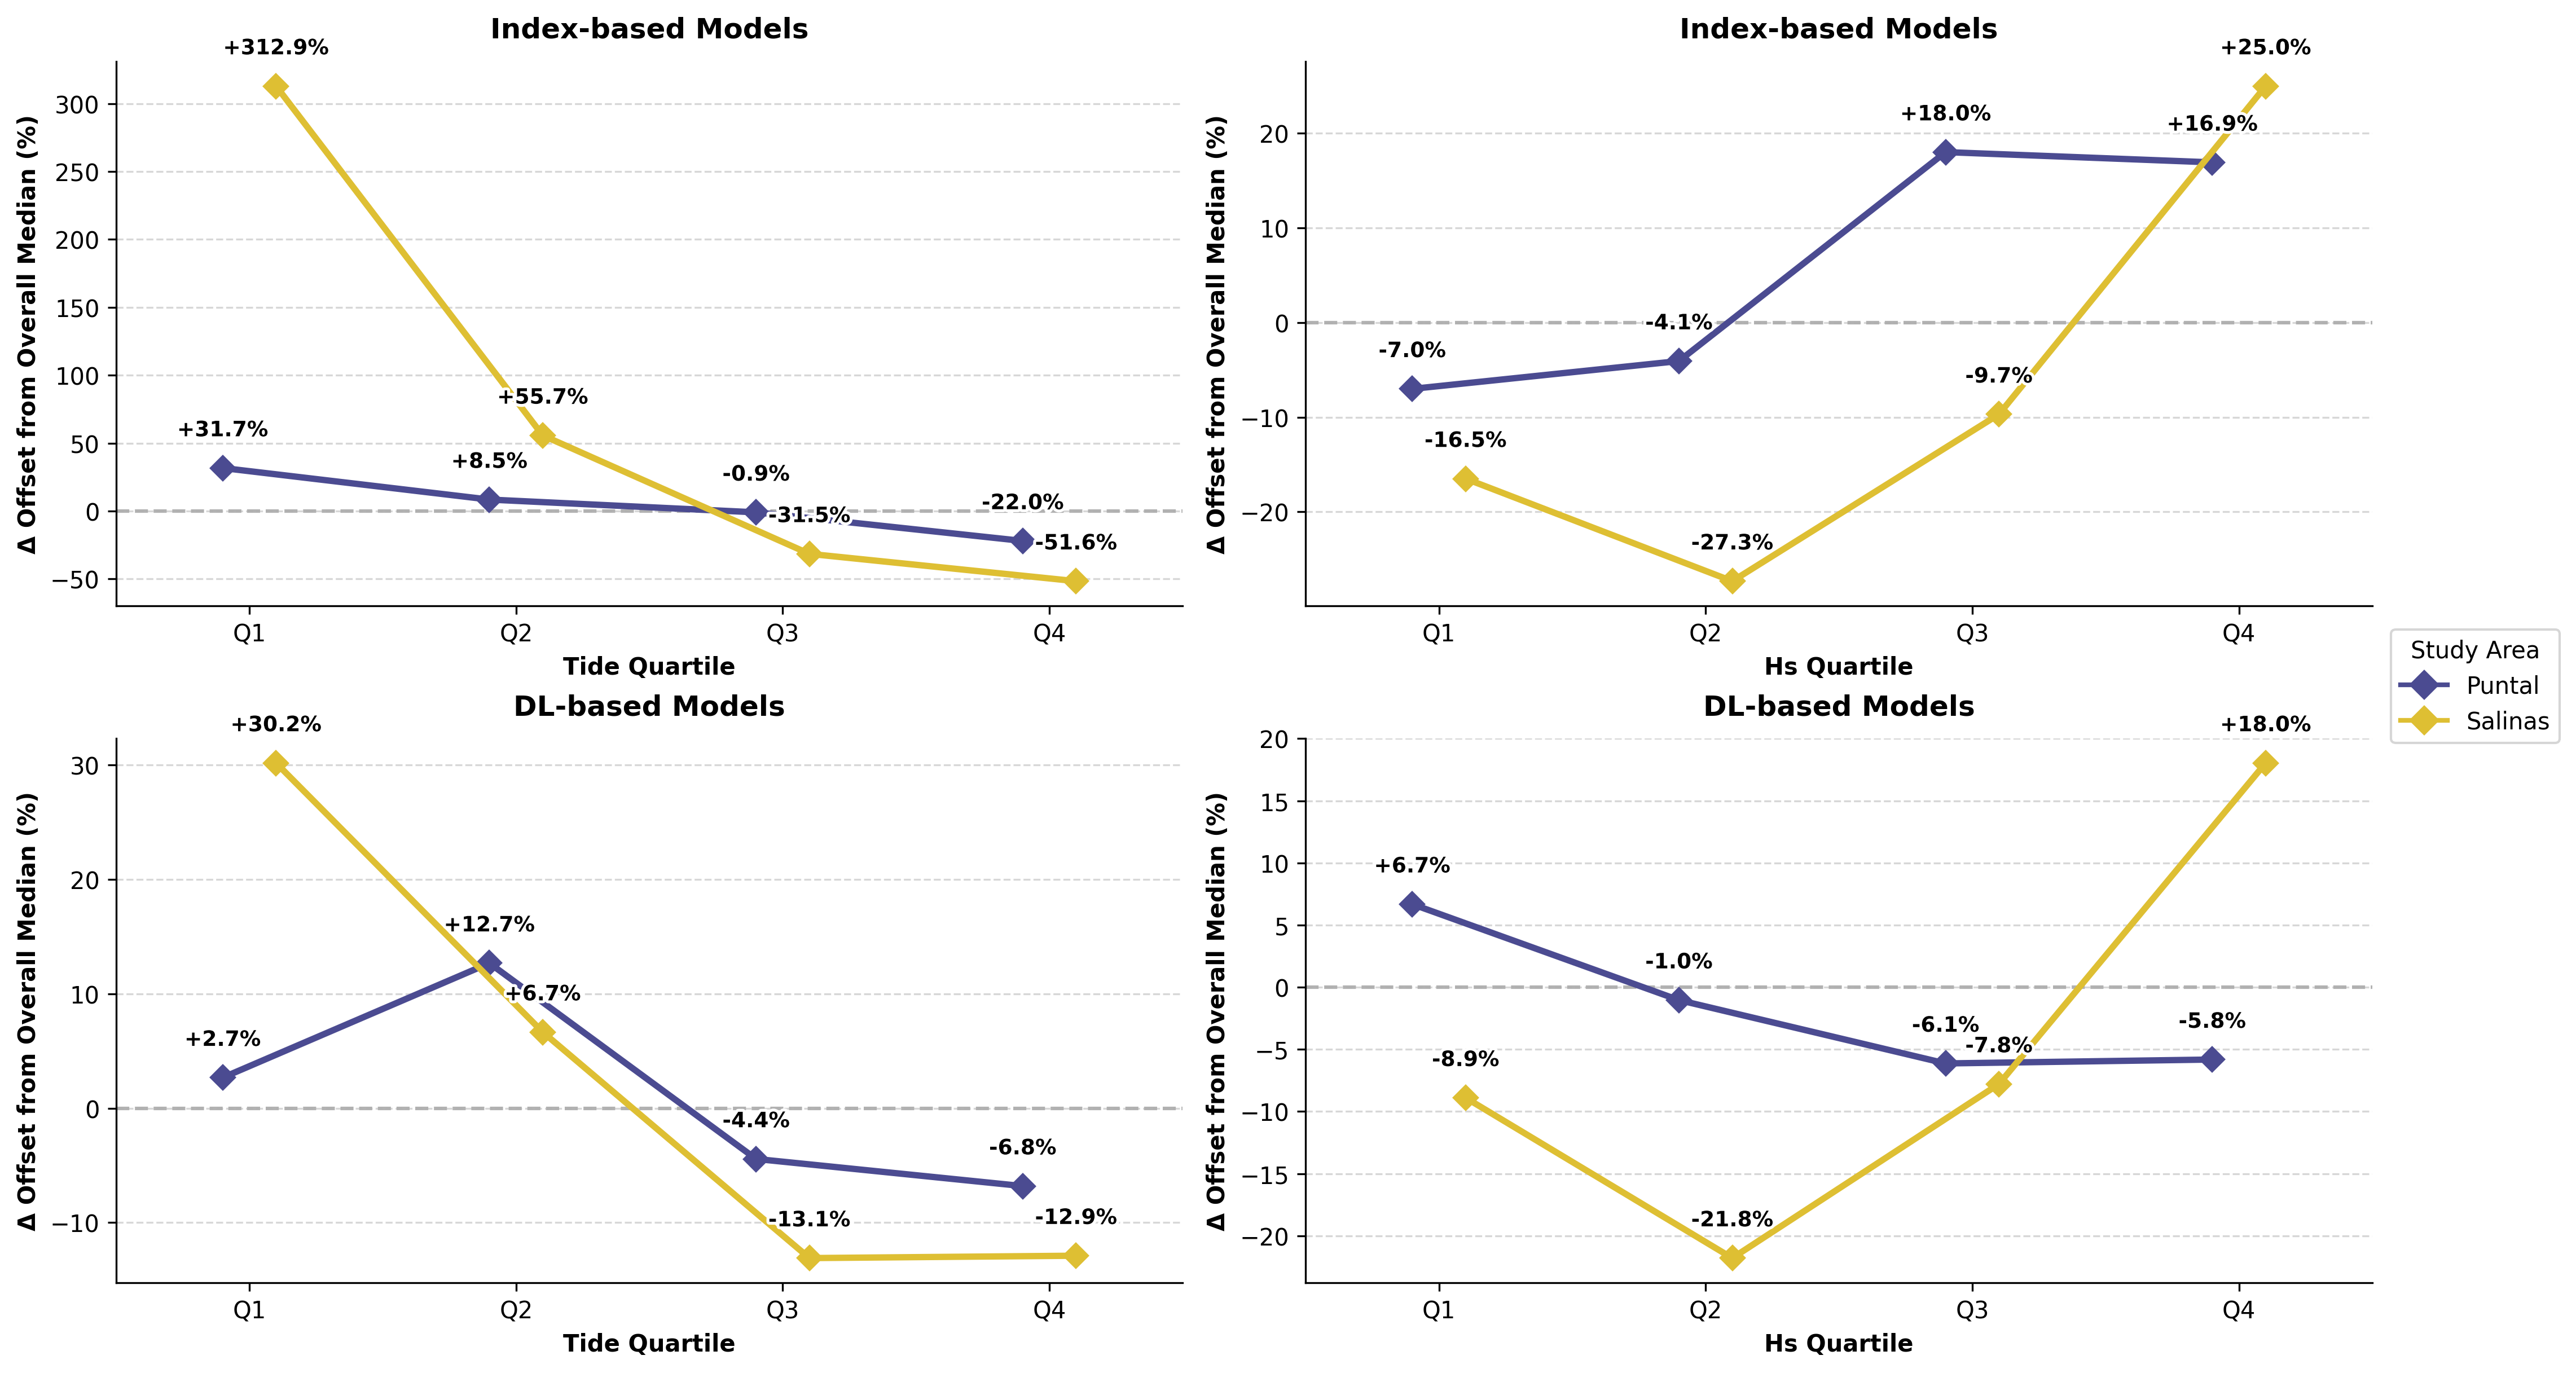
\includegraphics[width=\textwidth]{figure_pointplot_relative_quartiles.png}
    \caption{Relative performance sensitivity to hydrodynamic forcing. The plots display the percentage change in the median offset ($\Delta \%$) relative to the overall site median across astronomical tide (left) and significant wave height (right) quartiles. Index-based models (top row) show massive degradation during low tide (Q1) due to the exposed saturated intertidal zone. DL-based models (bottom row) demonstrate exceptional environmental resilience, maintaining highly stable predictions across all tidal and wave states.}
    \label{fig:quartiles_relative}
\end{figure}

% Responde a la Q3: Demuestra si el error aumenta drásticamente durante pleamares o eventos de alto oleaje.
% Gráficos del notebook:
% 1. Los boxplots del offset distribuidos a lo largo del transect_id para ver zonas críticas locales.
% 2. El panel de Stripplots + Pointplots agrupados por cuartiles de marea (tide_quartile) y de oleaje (hs_quartile).

\subsection{Cross-Site Generalization and Robustness}
\label{subsec:cross_site_generalization}
% Responde a la Q4: Identifica qué modelos se "sobreajustan" a las condiciones fáciles (Puntal) y fracasan en el stress-test (Salinas).
% Gráficos del notebook: El Lollipop Chart (horizontal) que muestra la diferencia (Delta MAE) entre Puntal y Salinas.

\section{Final Multi-Criteria Ranking}
\label{sec:final_ranking}
% Responde a la Q5: Síntesis de todo el apartado anterior combinando todas las métricas en un único sistema de puntuación.
% Gráficos del notebook:
% 1. El Heatmap final combinado (overall_df_combined) con todas las métricas normalizadas.
% 2. El Bump Chart (Ranking de líneas) que corona a los tres mejores modelos globales con estrellas.

\chapter{Conclusions and Future Works}

TO BE WRITTEN

%\section{Conclusions}
This chapter must include:
\begin{itemize}
\item A description of the conclusions of the work:
\begin{itemize}
    \item Once the results have been obtained, what conclusions are drawn?
    \item Are these results as expected? Or have they been amazing? Why?
\end{itemize}
\item A critical reflection on the achievement of the objectives initially set:
\begin{itemize}
    \item Have we achieved all the objectives? If the answer is negative, why?
\end{itemize}
\item A critical analysis of the monitoring of planning and methodology throughout the product:
\begin{itemize}
    \item Has the schedule been followed?
    \item Has the planned methodology been adequate enough?
    \item Has it been necessary to introduce changes to ensure the success of the work? Why?
\end{itemize}
\item From the impacts foreseen in \ref{s:etic}, ethical-social, sustainability and diversity, evaluate/mention whether they have been mitigated (if they were negative) or whether they have been achieved (if they were positive). 
\item If unforeseen impacts have appeared in \ref{s:etic}, evaluate/mention how they have mitigated (if they were negative) or what they have contributed (if they were positive).
\item The future lines of work that have not been explored in this work and have remained pending.


%\item A description of the conclusions of the work: What lessons have been learned from work?
%\item A critical reflection on the achievement of the objectives initially set: Have we achieved all the objectives? If the answer is negative, why?
%\item Of the impacts foreseen in the section \ref{s:etic}, an assessment, or at least mention, of whether they have been mitigated (if they were negative) or whether they have been achieved (if they were positive). 
\end{itemize}

%\section{Future Lines}
%The future lines of work that could not be explored in this work and have been pending.

%\section{Schedule Tracking}
%A critical analysis of the monitoring of the planning and methodology throughout the work: 
%\begin{itemize}
%    \item  Have the schedule been followed? 
%    \item Has the planned methodology been adequate? 
%    \item Has it been necessary to introduce changes to ensure the success of the work? Why?
%\end{itemize}

\chapter{Glossary}

TO BE WRITTEN

Definition of the most relevant terms and acronyms used in the Report.

%Defining the most relevant terms and acronyms used within the Memory.

\bibliographystyle{apalike}
\bibliography{references}

\newpage
\appendix
List of sections that are too extensive to include in memory and have a self-contained character (e.g. user manuals, installation manuals, etc.)
 
Depending on the type of work, there may be no need to add an annex.

\end{document}

